%
% Apunte de Sistemas Operativos
% Copyright (C) 2014 Esteban De La Fuente Rubio (esteban[at]delaf.cl)
%
% Permission is granted to copy, distribute and/or modify this document
% under the terms of the GNU Free Documentation License, Version 1.3
% or any later version published by the Free Software Foundation;
% with no Invariant Sections, no Front-Cover Texts, and no Back-Cover Texts.
% A copy of the license is included in the section entitled "GNU
% Free Documentation License".
%
% Link: http://www.gnu.org/copyleft/fdl.html
%

% se define estilo del documento
\documentclass[letterpaper,openright,12pt,leqno,onecolumn,twoside,openbib,titlepage]{book}

% PAQUETES
% codificación
\usepackage[utf8]{inputenc}
\usepackage[english,spanish]{babel}
% imágenes y gráficos
\usepackage{graphicx}
\usepackage{subfigure}
\usepackage{pdfpages}
\usepackage{tikz}
\usepackage{pgfplots}
\usepgflibrary{arrows}
\usetikzlibrary{shapes.multipart}
\usepackage{lib/pgf-thread}
% otros
\usepackage{hyperref}
\usepackage{enumerate}
\usepackage[section]{placeins}
\usepackage{verbatim}
\usepackage{booktabs}
\usepackage{fancyhdr}
\usepackage{listings}
\usepackage{color}

% MÁRGENES
\usepackage{anysize}
% izq, der, arr, abj
\marginsize{3cm}{2cm}{2cm}{3cm}

% INTERLINEADO
\renewcommand{\baselinestretch}{1.5}

% ENCABEZADO Y PIE DE PÁGINA
\pagestyle{fancy}
\lfoot{\today}
\cfoot{}
\rfoot{pág. \thepage}
\renewcommand{\headrulewidth}{0.4pt}
\renewcommand{\footrulewidth}{0.4pt}

% AJUSTES AL ÍNDICE
% hasta que sección se enumerará (section, subsection, subsubsection y
% párrafos)
\setcounter{secnumdepth}{3}
% hasta que nivel se agregará el índice (chapter, section, subsection,
% subsubsection y párrafos)
\setcounter{tocdepth}{2}

% OPCIONES PARA CÓDIGO FUENTE
% http://en.wikibooks.org/wiki/LaTeX/Source_Code_Listings
\definecolor{green}{rgb}{0,0.6,0}
\definecolor{gray}{rgb}{0.5,0.5,0.5}
\definecolor{mauve}{rgb}{0.58,0,0.82}
\lstset{
	xleftmargin=\parindent,
	language=C,
	commentstyle=\color{gray},
	keywordstyle=\color{blue},
	numbers=left,
	numbersep=10pt,
	numberstyle=\color{gray},
	stringstyle=\color{red},
	tabsize=2,
	showspaces=false,
	showstringspaces=false,
}

% INICIO DEL DOCUMENTO
\begin{document}

% PORTADA
\include{otros/portada}

% páginas que no son parte del contenido del libro en números romanos
\frontmatter

% LICENCIA
\include{otros/licencia}
% AGRADECIMIENTOS
%
% Apunte de Sistemas Operativos
% Copyright (C) 2014 Esteban De La Fuente Rubio (esteban[at]delaf.cl)
%
% Permission is granted to copy, distribute and/or modify this document
% under the terms of the GNU Free Documentation License, Version 1.3
% or any later version published by the Free Software Foundation;
% with no Invariant Sections, no Front-Cover Texts, and no Back-Cover Texts.
% A copy of the license is included in the section entitled "GNU
% Free Documentation License".
%
% Link: http://www.gnu.org/copyleft/fdl.html
%

% AGRADECIMIENTOS
\chapter*{Agradecimientos}
Son varias las personas que me han ayudado y apoyado durante los años, varios
durante el tiempo que llevo escribiendo este apunte, y justamente gracias a
algunos de ellos es que decidí escribirlo en ``formato libro''. Algunos son:

Al profesor Gabriel Astudillo, ya que con su apoyo y motivación fomentó en mi la
parte práctica en sistemas operativos \textit{like Unix}.

Al profesor Carlos Abarzúa, quién fue la persona que me introdujo en el área de
teoría de los sistemas operativos.

Al profesor Guillermo Badillo, quién confió en mi por primera vez para dictar el
curso de Sistemas Operativos en la Universidad Andrés Bello.

Al profesor Luis Mateu, quién me aceptó como oyente\footnote{Fui oyente en otoño
2012, su alumno en otoño 2013, su auxiliar en primavera 2013 y otoño 2014.} en
sus clases de Sistemas Operativos en la Universidad de Chile y en cuyas clases
se basó gran parte de este documento.

Además quisiera agradecer a todos aquellos que han permitido que este proyecto
salga adelante, ya sea con sus aportes, su ánimo o su paciencia (sobre todo
alumnos).

Adicionalmente agradeceré a cualquier lector que me indique sugerencias sobre el
contenido, reportes de errores o solicitud de algún tema que haya sido omitido o
no cubierto en la profundidad esperada. La idea es evaluar estos comentarios y
hacer los respectivos cambios en futuras versiones del documento.

% PÁGINA EN BLANCO
\newpage
\mbox{}
\thispagestyle{empty}

% RESUMEN
\include{otros/resumen}

% ÍNDICE
\tableofcontents
\listoffigures
\addcontentsline{toc}{chapter}{Índice de figuras}
\listoftables
\addcontentsline{toc}{chapter}{Índice de cuadros}

% desde aquí parte la pagina número 1
\mainmatter
\pagenumbering{arabic}

% CAPÍTULO 1: INTRODUCCIÓN
\include{capitulos/C01_introduccion}

% CAPÍTULO 2: HISTORIA
\include{capitulos/C02_historia}

% CAPÍTULO 3: ESTRUCTURA Y DISEÑO
\include{capitulos/C03_estructura}

% CAPÍTULO 4: PROCESOS
\include{capitulos/C04_procesos}

% CAPÍTULO 5: SINCRONIZACIÓN
%
% Apunte de Sistemas Operativos
% Copyright (C) 2014 Esteban De La Fuente Rubio (esteban[at]delaf.cl)
%
% Permission is granted to copy, distribute and/or modify this document
% under the terms of the GNU Free Documentation License, Version 1.3
% or any later version published by the Free Software Foundation;
% with no Invariant Sections, no Front-Cover Texts, and no Back-Cover Texts.
% A copy of the license is included in the section entitled "GNU
% Free Documentation License".
%
% Link: http://www.gnu.org/copyleft/fdl.html
%

% WARNING: caracteres especiales (como eñes y acentos) han sido omitidos a
% propósito al utilizar lstlisting, ya que este paquete no soporta UTF-8.

% SINCRONIZACIÓN
\chapter{Sincronización}
\label{sincronizacion}

Este capítulo se centra en mecanismos de sincronización entre procesos, esto
con el objetivo de solucionar los problemas descritos anteriormente:
\emph{dataraces}, \emph{deadlock} y \emph{starvation}.

Se mostrará primero la forma incorrecta de solucionar los problemas de exclusión
mutua, utilizando \emph{busy-waiting}. Luego se presentarán los problemas
clásicos estudiados en sistemas operativos, estos son ``productor consumidor'',
``cena de filósofos'' y ``lectores escritores''. Finalmente se introducirán tres
herramientas de sincronización, las cuales corresponden a semáforos, monitores y
mensajes.

\section{\emph{Busy-waiting}}
Una solución a los problemas de exclusión mutua es consultar reiteradamente si
el recurso que se está solicitando está o no disponible. Son interesantes, ya
que permiten entender porque son incorrectas y que las hace inapropiadas para el
problema de exclusión mutua.

Una de las posibles soluciones es utilizar una bandera o \emph{flag} para
indicar si la sección crítica esta (1) o no (0) siendo ocupada.

\begin{lstlisting}
int bandera = 0;
int contador = 0;
void aumentar()
{
	while (bandera);
	bandera = 1;
	int aux = contador;
	contador = aux + 1;
	bandera = 0;
}
\end{lstlisting}

\begin{enumerate}[a)]

\item \textbf{¿Qué sucede con la variable global bandera?} al ser compartida y
accedida (para lectura y modificación) por más de un proceso se convierte
también  en una sección crítica vulnerable \emph{data races}. O sea, lo que
se pretendía usar para controlar a sección crítica se convierte en una sección
rítica.

\item \textbf{¿Qué ocurre si dos procesos consultan en el \texttt{while} y la
bandera es 0?} Puede ocurrir que el primer proceso sea interrumpido justo
después del \texttt{while} y, al no alcanzar a poner la bandera en 1, el segundo
proceso también entre a la sección crítica que se quiere proteger.

\end{enumerate}

Existen diversas soluciones para el problema de exclusión mutua utilizando
\emph{busy-waiting}. Se pueden revisar los algoritmos de Dekker y Peterson
para más soluciones de este tipo.

El gran problema con las soluciones de \emph{busy-waiting} es que realizan una
\textbf{espera activa} del recurso. Esto significa que utilizan CPU para
consultar cada vez por el recurso. Lo que se verá en el resto del capítulo serán
herramientas de sincronización con \emph{espera pasiva}, donde el proceso
consulta, y si el recurso está ocupado se ``duerme''.

Es importante destacar que la espera activa es el problema de todas las
soluciones que utilizan \emph{busy-waiting}, sin embargo pueden existir
soluciones de este tipo que a pesar de este problema sean correctas para
realizar la sincronización.

\section{Problemas clásicos}
En la literatura relacionada con sistemas operativos generalmente se mencionan
tres problemas clásicos, los cuales se enunciarán a continuación y serán
utilizados durante los ejemplos de los diferentes métodos de sincronización.

\subsection{Productor consumidor}
En el problema del productor consumidor, o \emph{buffer} acotado, existe uno o
varios productores que \textbf{producen cierto elemento} mientras que uno o
varios consumidores \textbf{consumen dicho elemento}. Las operaciones
\emph{put} y \emph{get} se realizan sobre una pila finita y los
elementos deben ser entregados en el mismo orden en que fueron depositados.

A continuación se muestra una visión global del problema, posteriormente una
solución incorrecta. Soluciones correctas serán vistas cuando se estudien los
diferentes mecanismos de sincronización.

Versión secuencial (no interesante):
\begin{lstlisting}
void productor_consumidor ()
{
  for (;;) {
    item it = produce();
    consume(it);
  }
}
\end{lstlisting}

Versión paralela (interesante):
\begin{lstlisting}
void productor ()
{
  for (;;) {
    item it = produce();
    put(it);
  }
}
void consumidor ()
{
  for (;;) {
    item it = get();
    consume(it);
  }
}
\end{lstlisting}

Restricciones:
\begin{itemize}

\item \emph{get} no puede entregar \emph{items} que no fueron suministrados
con \emph{put} (se deberá bloquear el consumidor si no hay items).

\item Con \emph{put} se pueden recibir hasta $N$ \emph{items} sin que hayan
sido extraídos con \emph{get} (se deberá bloquear del productor si la pila
está llena).

\item \emph{Items} tienen que ser extraídos en el mismo orden en que fueron
depositados.

\item Tiene que funcionar en paralelo (no sirve versión secuencial).

\end{itemize}

Las funciones \emph{produce} y \emph{consume} son lentas y pueden ser
ejecutadas en paralelo sin ningún problema (ya que no interactuan al mismo
tiempo con otros procesos sobre algún recurso compartido). La solución deberá
considerar la implementación sincronizada de \emph{put} y \emph{get},
asumiendo el resto de funciones como dadas (o sea, existen y funcionan).

\begin{figure}[htbp]
	\centering
	\selectlanguage{english}
	\begin{tikzpicture}
		% formatos
		\tikzstyle{productor} = [draw, circle, node distance=4cm]
		\tikzstyle{consumidor} = [draw, circle, node distance=4cm]
		\tikzstyle{stack} = [draw, rectangle split, rectangle split
horizontal, rectangle split parts=10]
		\tikzstyle{arrow} = [->, semithick, auto]
		% productores y consumidores
		\node [productor]  (P1)
	  {P1};
		\node [productor]	 (P2)	[right of =P1]	{P2};
		\node [consumidor] (C1)	[right of =P2]	{C1};
		\node [consumidor] (C2) [right of =C1]  {C2};
		% stack
		\node at (6, -2) [stack] (stack) {
			\nodepart{six}X
			\nodepart{seven}X
		};
		% relaciones
		\draw [arrow] (P1) to node {put} (stack);
		\draw [arrow] (P2) to node {put} (stack);
		\draw [arrow] (stack) to node {get} (C1);
		\draw [arrow] (stack) to node {get} (C2);
	\end{tikzpicture}
	\selectlanguage{spanish}
	\caption{Interacción entre productores y consumidores}
	\label{fig:interaccion_productores_consumidores}
\end{figure}

\subsubsection{Solución incorrecta: \emph{data races}}

\begin{lstlisting}
#define N 100
Item buffer[N];
int e = 0;
int f = 0;
int c = 0;
void put (Item item)
{
  while(c==N);
  buffer[e] = item;
  e = (e+1) % N;
  c++;
}
Item get ()
{
  Item item;
  while(c==0);
  item = buffer[f];
  f = (f+1) % N;
  c--;
  return item;
}
\end{lstlisting}

\textbf{¿Por qué la solución anterior es incorrecta?} Al utilizar una variable
global $c$ para indicar la cantidad de elementos que hay en la pila, se incurre
en el problema de exclusión mutua, donde si no hay sincronización la variable
$c$ podría sufrir problemas de \emph{data races} y quedar en un estado
inconsistente durante algún punto de la ejecución. Adicionalmente la solución
considera el uso de \emph{busy-waiting} lo cual ya se discutió que no es
aceptable.

\subsection{Cena de filósofos}
Se ha invitado a una cena a cinco filósofos chinos a comer y pensar, donde
realizan solo una de estas actividades al mismo tiempo. En la mesa donde se han
de sentar existen 5 puestos y 5 palitos (o tenedores, dependiendo de la
bibliografía).

\begin{figure}[htbp]
\centering
\includegraphics[scale=1.00]{img/C05_sincronizacion/filosofos.png}
\caption{Problema cena de filósofos}
\label{fig:concurrencia_filosofos}
\end{figure}

Restricciones:
\begin{itemize}
\item Cada filósofo solo puede tomar palitos que están a su lado.
\item Un filósofo requiere dos palitos para comer.
\item Un palito no puede ser utilizado por dos filósofos al mismo tiempo.
\end{itemize}

\subsubsection{Solución incorrecta: \emph{data races}}
\begin{lstlisting}
void filosofo (int i)
{
  for(;;) {
    comer(i, (i+1)%5);
    pensar();
  }
}
\end{lstlisting}

El problema en esta solución ocurre por el uso de la función comer
directamente con $i$ e $i+1$, dos filósofos podrían tomar el mismo palito.

\subsection{Lectores escritores}
Este problema utiliza la idea de un diccionario, se dispone de dos arreglos de
tamaño fijo donde uno contiene las palabras del diccionario y el otro sus
definiciones. Se mostrarán los prototipos (o firmas) de funciones para poder
agregar una nueva definición al diccionario, para consultar por una definición y
para eliminar una definición.

Restricciones:
\begin{itemize}
\item $n$ lectores o escritores requieren acceso a una estructura de datos
compartida.
\item Los lectores solo consultan.
\item Los escritores modifican la estructura de datos.
\item Lectores y escritores deberán utilizar herramientas de sincronización ya
que si bien múltiples lectores pueden trabajar sobre la estructura, solo un
escritor puede hacerlo en un determinado tiempo.
\end{itemize}

Suponga la siguiente API:
\begin{lstlisting}
void newDef (char *k, char *d);
char *query (char *k);
void delDef (char *k);
\end{lstlisting}

Un ejemplo del uso de la API se ilustra a continuación:
\begin{lstlisting}
newDef("a", "1");           /* se crea palabra "a" con definicion "1" */
printf("%s\n", query("a")); /* imprime: 1 */
delDef("a");                /* se elimina la palabra a */
printf("%s\n", query("a")); /* NULL */
\end{lstlisting}

Se debe implementar la API de tal forma de cumplir con los requisitos y
restricciones del problema.

\subsubsection{Solución incorrecta: \emph{data races}}
\begin{lstlisting}
/* Definicion de arreglos globales para palabras y definiciones */
#define MAX 100
char *keys[MAX], *defs[MAX];

/* Funcion que obtiene una casilla vacia */
int getSlot ()
{
  int i;
  for(i=0; i<MAX; i++)
    if(keys[i]==NULL)
      return i;
  return -1;
}

/* Funcion que crea una nueva definicion en el diccionario */
void newDef (char *k, char *d)
{
  int i = getSlot();
  if(i!=-1) {
    keys[i] = k;
    defs[i] = d;
  }
}

/* Funcion que obtiene la posicion en la casilla a partir de una clave */
int getIdX (char *k)
{
  int i;
  for(i=0; i<MAX; i++)
    if(keys[i]!=NULL && !strcmp(k, keys[i]))
      return i;
  return -1;
}

/* Funcion que recupera una definicion */
char *query (char *k)
{
  int i = getIdX(k);
  return i==-1 ? NULL : defs[i];
}

/* Funcion que elimina una definicion del diccionario */
void delDef (char *k)
{
  int i = getIdX(k);
  if(i!=-1) {
    keys[i] = NULL;
    defs[i] = NULL;
  }
}
\end{lstlisting}

Al analizar el código se observa que pueden ocurrir \emph{data races} si se
realizan al menos dos modificaciones en paralelo o si se realiza una
modificación con una consulta. No ocurrirán problemas si se realizan dos
consultas en paralelo.

Algunas de las situaciones anómalas se describen a continuación (el lector
deberá considerar que otros problemas pueden ocurrir).

\begin{enumerate}[i.]

\item \textbf{\texttt{newDef} con \texttt{newDef}}: al realizar una nueva
definición se consulta por una casilla libre, si justo en el momento después de
consultar si la casilla está libre (instrucción \texttt{if} en
\texttt{getSlot}), se saca al proceso de la CPU y entra otro proceso que hace la
misma consulta se podría entregar la misma casilla a ambos procesos.

\item \textbf{\texttt{query} con \texttt{delDef}}: al seleccionar una
definición se consulta mediante \texttt{getIdX} el índice dentro del arreglo, si
justo después de consultar por el índice se saca al proceso de la CPU y se llama
a \texttt{delDef} eliminando la misma definición consultada, cuando
\texttt{query} retome la CPU y use el índice obtenido no estará lo esperado en
la casilla.

\item \textbf{\texttt{query} con \texttt{newDef}}: el resultado de
\texttt{query} puede ser \texttt{NULL} si se ejecuta antes que \texttt{newDef} o
distinto de \texttt{NULL} si se ejecuta después.

\end{enumerate}

\section{Semáforos}
Los \textbf{semáforos} corresponden básicamente a contadores (de
\emph{tickets}), donde para utilizar una sección crítica se consulta por el
valor del semáforo, si este es mayor a cero (o sea hay tickets) se usa la
sección, si es igual a cero, se deberá esperar.

El valor del semáforo (o la cantidad de tickets) será inicializado,
generalmente, en la cantidad de procesos que pueden hacer uso al mismo tiempo de
la sección crítica. Adicionalmente las rutinas utilizadas deben ser atómicas,
esto para garantizar que varios procesos puedan consultar el valor del semáforo
sin que ocurran \emph{data races}.

\begin{lstlisting}
s=1;
void proceso ()
{
 solicitar_ticket(s);
 // ejecucion de seccion critica
 liberar_ticket(s);
}
\end{lstlisting}

Los procesos que no tengan acceso al semáforo, por falta de \emph{tickets},
deberán esperar en una cola FIFO a que se depositen \emph{tickets}, en cuyo
momento se despertará al proceso que estaba primero en la cola para que obtenga
el \emph{ticket} del semáforo y entre en la sección crítica.

\subsection{API}

\begin{lstlisting}
/* Inicializa el semaforo */
struct semaphore *semaphore_make (int tickets);

/* Solicita el semaforo */
void semaphore_wait (struct semaphore *s);

/* Libera el semáforo */
void semaphore_signal (struct semaphore *s);
\end{lstlisting}

\subsection{Modo de operación}
Un bosquejo de la implementación de las funciones de la API que ayudará a
comprender como operan los semáforos es la siguiente:

\begin{lstlisting}
void wait (s)
{
  s--;
  if(s < 0)
    block(s);     /* suspender proceso y agregarlo al final de la cola */
}
void signal (s)
{
  s++;
  if (s <= 0)
    wakeup(s);    /* despertar primer proceso en la cola */
}
\end{lstlisting}

\textbf{¿Qué significa que el valor del semáforo sea -1?}, significaría que ya
hay un proceso antes en la cola FIFO. Por lo cual al recibir un \texttt{signal}
se despertará primero al otro proceso.

Una implementación real, utilizando \texttt{nSystem}\footnote{Sistema
Operativo de juguete desarrollado por el profesor Luis Mateu de la Universidad
de Chile}, puede ser vista en el anexo \ref{nSystem}.

\subsection{Problema productor consumidor}

\subsubsection{Solución correcta}

\begin{lstlisting}
#define N 100
Item buffer[N];
int e = 0;
int f = 0;
struct semaphore *empty; /* = semaphore_make (N) */
struct semaphore *full;  /* = semaphore_make (0) */
void put (Item item)
{
  semaphore_wait (empty);
  buffer[e] = item;
  e = (e+1) % N;
  semaphore_signal (full);
}
Item get ()
{
  Item item;
  semaphore_wait (full);
  item = buffer[f];
  f = (f+1) % N;
  semaphore_signal (empty);
  return item;
}
\end{lstlisting}

Esta solución es válida para un productor y un consumidor. Para $n$ productores
y $m$ consumidores se debe definir un semáforo adicional para cubrir la sección
crítica tanto de la función \texttt{put} como de la función \texttt{get}. Esto
queda de tarea al lector.

\subsection{Problema cena de filósofos}

\subsubsection{Solución incorrecta: \emph{deadlock}}

\begin{lstlisting}
struct semaphore s[5]; /* for(i=0; i<5; i++) s[i] = semaphore_make (1); */
void filosofo (int i)
{
  for(;;) {
    semaphore_wait (s[i]);
    semaphore_wait (s[(i+1)%5]);
    comer (i, (i+1)%5);
    semaphore_signal (s[i]);
    semaphore_signal (s[(i+1)%5]);
    pensar ();
  }
}
\end{lstlisting}

El problema en esta solución es lo que sucedería si todos los filósofos
solicitaran el palito $i$ ``al mismo tiempo'', cuando quieran solicitar el
palito $i+1$ ya alguien lo tendrá tomado.

\subsubsection{Solución correcta específica}
Se debe evitar que entren los 5 filósofos al mismo tiempo a la mesa, con esto se
asegurará que al menos uno de ellos coma. En este caso la misma mesa se
convierte en una sección crítica.

\begin{lstlisting}
struct semaphore *m;    /* m = semaphore_make (4); */
struct semaphore s[5];  /* for(i=0; i<5; i++) s[i] = semaphore_make (1); */
void filosofo (int i)
{
  for(;;) {
    semaphore_wait (m);
    semaphore_wait (s[i]);
    semaphore_wait (s[(i+1)%5]);
    comer (i, (i+1)%5);
    semaphore_signal (s[i]);
    semaphore_signal (s[(i+1)%5]);
    semaphore_signal (m);
    pensar ();
  }
}
\end{lstlisting}

\subsubsection{Solución correcta general}
Se deben solicitar los recursos siempre en el mismo orden, ya sea ascendente o
descendente. Esto evitará el interbloqueo.

\begin{lstlisting}
struct semaphore s[5];  /* for(i=0; i<5; i++) s[i] = semaphore_make (1); */
void filosofo (int i)
{
  int min = min (i, (i+1)%5);
  int max = max (i, (i+1)%5);
  for(;;) {
    semaphore_wait (s[min]);
    semaphore_wait (s[max]);
    comer(min, max);
    semaphore_signal (s[min]);
    semaphore_signal (s[max]);
    pensar();
  }
}
\end{lstlisting}

Asumamos que entra el filósofo 2, solicitará el palito 2 y el palito 3 y comerá.
Luego entra el filósofo 1, solicita el palito 1 (está disponible), pero al pedir
el palito 2 (que esta ocupado por el filósofo 2) se bloquea a la espera que se
desocupe. El problema aquí es que el filósofo 1 espera reteniendo el palito 1,
entonces si llega un filósofo 0, que puede usar el palito 0, el palito 1 no lo
conseguirá a pesar de que no está siendo utilizado para comer (solo está siendo
retenido por el filósofo 1). Eventualmente, cuando el filósofo 2 libere el
palito 2, el filósofo 1 comerá y eventualmente el 0 también lo hará. Sin embargo
¿podría haber comido el 2 y el 0 al mismo tiempo?, la respuesta es sí.

El problema de los semáforos, en general, es que no se puede saber si el
semáforo está o no ocupado antes de pedirlo. Esto trae como consecuencia una
limitación del paralelismo, ya que al consultar por el palito este es retenido
independientemente de si el otro está o no disponible. Sin embargo, si se
considera que la operación comer es mucho más rápida que la de pensar, por
ejemplo asumiendo que comer es leer datos y pensar es procesarlos, esta
limitación de paralelismo no es tan grave para ciertos problemas.

Lo anterior se podría solucionar implementando ``algo'' que permita pedir dos
semáforos al mismo tiempo, pero que no los deje tomados si uno de ellos está
ocupado. Esto entregará un mayor paralelismo, pero introducirá el problema de
hambruna, donde dos filósofos (por ejemplo filósofos 0 y 2) podrían estar
pidiendo siempre los palitos que un tercero (filósofo 1) quisiera utilizar.

\section{Monitores de Brinch Hansen}
Los \textbf{monitores} de Brinch
Hansen\footnote{\url{http://es.wikipedia.org/wiki/Per_Brinch_Hansen}} son una
herramienta de sincronización que ofrece más paralelismo que los semáforos, pero
pueden provocar hambruna. Permitirán consultar al mismo tiempo por el valor de
más de una condición, si alguno de los elementos de dicha condición no se cumple
de la forma requerida el proceso se suspenderá.

Los monitores pueden ser vistos como semáforos binarios, donde el
``\emph{ticket}'' del monitor es la propiedad del mismo.

\begin{lstlisting}
void proceso ()
{
 solicitar_propiedad(m);
 // ejecución de sección crítica
 liberar_propiedad(m);
}
\end{lstlisting}

Es importante mencionar que la propiedad del monitor debe ser devuelta siempre
por el mismo proceso que la solicitó.

\subsection{API}

\begin{lstlisting}
/* Crear un monitor */
struct monitor *monitor_make ();

/* Destruir un monitor */
void monitor_destroy (struct monitor *m);

/* Solicitar la propiedad sobre un monitor */
void monitor_enter (struct monitor *m);

/* Devuelve la propiedad del monitor */
void monitor_exit (struct monitor *m);

/* Devuelve la propiedad y suspende el proceso hasta un monitor_notify_all  */
void monitor_wait (struct monitor *m);

/* Despierta las tareas suspendidas con monitor_wait  que esperan la propiedad
del monitor */
void monitor_notify_all (struct monitor *m);
\end{lstlisting}

Un proceso que espera, suspendido, por la propiedad del monitor al haber usado
\texttt{monitor\_enter} esperará hasta que esta sea liberada por el proceso que
la ocupa, ya sea mediante un \texttt{monitor\_wait} o un \texttt{monitor\_exit}.

Al despertar procesos bloqueados por un \texttt{monitor\_enter} o un
\texttt{monitor\_wait} obtendrán la propiedad sin garantía del orden, o sea,
\textbf{monitores no son FIFO}. Igualmente, cuando se hace una llamada a
\texttt{monitor\_notify\_all} se despertarán todos los procesos suspendidos
por un \texttt{monitor\_wait} del mismo monitor, el orden en que despiertan no
está garantizado, o sea no necesariamente es FIFO respecto a la ejecución de
\texttt{monitor\_wait}. Adicionalmente una vez despertados los procesos deben
esperar la propiedad del monitor (esto ya que \texttt{monitor\_notify\_all}
solo despierta, no entrega la propiedad, la cual será entregada al usar
\texttt{monitor\_exit}) y evaluar nuevamente sus condiciones, si nuevamente no
se cumplen se suspenderán liberando el monitor, así otro proceso despertado con
\texttt{monitor\_notify\_all} podrá obtener la propiedad y también evaluar sus
condiciones nuevamente. Podría ocurrir también que con
\texttt{monitor\_notify\_all} los procesos al evaluar sus condiciones, ninguno
pueda continuar, y todos se vuelvan a suspender.

\subsection{Problema productor consumidor}

\subsubsection{Solución incorrecta: \emph{deadlock}}
\begin{lstlisting}
void put (Item it)
{
  monitor_enter (monitor);
  while (c==N);
  buffer[e] = it;
  e = (e+1) % N;
  c++;
  monitor_exit (monitor);
}
Item get ()
{
  Item it;
  monitor_enter (monitor);
  while(c==0);
  it = buffer[f];
  f = (f+1) % N;
  c--;
  monitor_exit (monitor);
  return it;
}
\end{lstlisting}

Suponga que $c=N$, o sea el productor no puede depositar más \emph{items} en
la pila y debe esperar. En este caso al ejecutar \texttt{put}, se solicitará la
propiedad del monitor y el proceso quedará en el ciclo del \texttt{while}, con
espera activa y con el monitor tomado. Si llega un consumidor y solicita la
propiedad sobre el monitor para extraer un \emph{item}, lo cual es válido por
la situación descrita, no podrá hacerlo, ya que el monitor está tomado por un
productor, el cual espera (la condición de su \texttt{while}) que un consumidor
extraiga al menos un \emph{item}. En este caso se produce el problema de
interbloqueo.

\subsubsection{Solución correcta}
Se debe buscar una solución que permita devolver el monitor si la condición de
espera se cumple, esto se logra utilizando \texttt{monitor\_wait} sobre el
monitor.

\begin{lstlisting}
void put (Item it)
{
  monitor_enter (monitor);
  while(c==N)
    monitor_wait (monitor);
  buffer[e] = it;
  e = (e+1) % N;
  c++;
  monitor_notify_all (monitor);
  monitor_exit (monitor);
}
Item get ()
{
  Item it;
  monitor_enter (monitor);
  while(c==0)
    monitor_wait (monitor);
  it = buffer[f];
  f = (f+1) % N;
  c--;
  monitor_notify_all (monitor);
  monitor_exit (monitor);
  return it;
}
\end{lstlisting}

Si llega un productor y ve que la pila está llena, hará espera pasiva y
devolverá la propiedad del monitor. Análogamente si un consumidor ve que la pila
está vacía esperará de forma pasiva y devolverá la propiedad del monitor. Esta
acción de devolver la propiedad del monitor y quedar en espera pasiva es lograda
mediante \texttt{monitor\_wait}. Adicionalmente se agrega la instrucción
\texttt{monitor\_notify\_all}, la cual despertará a todos los procesos
bloqueados mediante un \texttt{monitor\_wait} de dicho monitor, obtendrán la
propiedad y podrán evaluar nuevamente la condición de espera, si no se sale del
\texttt{while} se volverá a dormir entregando la propiedad a otro proceso para
que pueda continuar. Notar que no se puede determinar en que orden serán
despertados los procesos, por lo cual cualquier proceso podría tomar la
propiedad una vez sean despertados por \texttt{monitor\_notify\_all}.

\subsection{Patrón de solución usando monitores}

\begin{lstlisting}
... operacion (...)
{
  ...
  monitor_enter (m);
  while (!invariante)       /* condicion para quedar en espera */
    monitor_wait (m);
  ...                       /* operaciones */
  monitor_notify_all (m);   /* opcional, solo si las operaciones modifican
                               datos que afecten la condicion de otros que
			       esperan (además podría ir antes del while)
			     */
  monitor_exit (m);
  return ...;
}
\end{lstlisting}

Se recomienda aislar los distintos aspectos de la solución, separando el código
de sincronización del resto de la aplicación. Se verá esto a continuación en la
solución de la cena de filósofos.

\subsection{Problema cena de filósofos}
\subsubsection{Solución ``correcta''}
\begin{lstlisting}
/* llamadas a rutinas del filosofo */
void filosofo (int i)
{
  for(;;) {
    pedir (i, (i+1)%5);
    comer (i, (i+1)%5);
    devolver (i, (i+1)%5);
    pensar ();
  }
}

/* sincronizacion */

struct monitor *m;            /* m = monitor_make (); */
int ocup[5] = {0, 0, 0, 0, 0} /* =0 palito esta libre */

void pedir (int i, int j)
{
  monitor_enter (m);
  while(ocup[i] || ocup[j])
    monitor_wait (m);
  ocup[i] = ocup[j] = 1;
  monitor_exit (m);
}

void devolver (int i, int j) {
  monitor_enter (m);
  ocup[i] = ocup[j] = 0;
  monitor_notify_all (m);        /* DEBE ir, ya que se liberan los palitos */
  monitor_exit (m);
}
\end{lstlisting}

Esta solución evita que un filósofo retenga un palito sin estar comiendo (lo que
sucedía con semáforos), por lo cual aumenta el paralelismo. Sin embargo
introduce el problema de \textbf{hambruna}.

Suponga que en el tiempo 0 ingresa el filósofo 0, podrá comer con los palitos 0
y 1. Luego ingresa el filósofo 1 el cual no podrá comer ya que de los palitos
requeridos (1 y 2) el 1 ya esta siendo ocupado. Luego ingresa el filósofo 2 y
podrá comer (usando palitos 2 y 3). Resumiendo, $F_0$ y $F_2$ están comiendo,
mientras $F_1$ esta esperando a que los palitos (1 y 2) sean liberados. Suponga
ahora que después de un tiempo $F_0$ deja de comer, se notifica a $F_1$ que hay
palitos libres, sin embargo solo dispone del palito 1, por lo cual deberá seguir
esperando por el palito 2 y no podrá comer. Luego $F_0$ vuelve a pedir los
palitos, están libres y come. Ahora $F_2$ liberá los palitos, pero como $F_0$
volvió a pedir el palito 1, a pesar de tener el 2 libre $F_1$ no podrá comer.
Esta situación puede repetirse indefinidamente, donde por la ejecución de $F_0$
y $F_2$, $F_1$ podría nunca tener disponibles los 2 palitos que necesita para
poder comer.

Se deja al lector la tarea de mostrar mediante un diagrama de hebras la
situación de hambruna descrita anteriormente.

\subsection{Problema lectores escritores}

Las funciones \texttt{newDef} y \texttt{delDef} definirán un conjunto de
operaciones de escritura, donde su sección crítica será rodeada por un
\texttt{enterWrite} y \texttt{exitWrite} que se encargarán de realizar las
tareas de sincronización. Análogamente, la función \texttt{query} denotará una
operación de lectura, donde su sección crítica será rodeada por un
\texttt{enterRead} y \texttt{exitRead}.

A continuación se muestra el modo de uso de estas funciones de sincronización,
posteriormente se revisarán dos implementaciones de las mismas.

\begin{lstlisting}
/* Lector */
char *query (char *k)
{
  enterRead(); /* inicio seccion critica */
  int i = getIdX(k);
  char *aux = i==-1 ? NULL : defs[i];
  exitRead(); /* fin seccion critica */
  return aux;
}

/* Escritor */
void newDef (char *k, char *d)
{
  enterWrite(); /* inicio seccion critica */
  int i = getSlot();
  if(i!=-1) {
    keys[i] = k;
    defs[i] = d;
  }
  exitWrite(); /* fin seccion critica */
}
void delDef (char *k)
{
  enterWrite(); /* inicio seccion critica */
  int i = getIdX(k);
  if(i!=-1) {
    keys[i] = NULL;
    defs[i] = NULL;
  }
  exitWrite(); /* fin seccion critica */
}
\end{lstlisting}

El uso de funciones diferentes para acceder a la sección crítica en lecturas y
escrituras está relacionado con que varios lectores pueden consultar al mismo
tiempo la sección crítica, sin embargo no puede haber alguien más cuando
se hace una modificación (o sea, escritores deben trabajar solos).

\subsubsection{Solución ``correcta''}
\begin{lstlisting}
struct monitor *c;      /* = monitor_make () */
int readers = 0; /* contador de lectores leyendo */
int writing = 0; /* =0 no hay alguien escribiendo */

void enterRead ()
{
  monitor_enter (c);
  while(writing) /* se pregunta si alguien esta escribiendo */
    monitor_wait (c);
  readers++;     /* se indica que entro un lector */
  monitor_exit (c);
}

void exitRead ()
{
  monitor_enter (c);
  readers--;
  monitor_notify_all (c); /* avisa a escritores que podrian entrar */
  monitor_exit (c);
}

void enterWrite ()
{
  monitor_enter (c);
  while(readers>0 || writing)
    monitor_wait (c);
  writing = 1;   /* se indica que un escritor esta trabajando */
  monitor_exit (c);
}

void exitWrite ()
{
  monitor_enter (c);
  writing = 0;
  monitor_notify_all (c); /* avisa a lectores o escritores que podrian entrar */
  monitor_exit (c);
}
\end{lstlisting}

Recordar que al utilizar \texttt{monitor\_exit} se libera la propiedad del
monitor y alguno de los que estaba esperándola la tomará, sin embargo no se
especifica cual proceso será (recordar, no hay orden FIFO).

Si ``llegan y llegan'' lectores, los cuales pueden leer en paralelo, y nunca el
contador \texttt{readers} es 0, ningún escritor podrá acceder a la sección
crítica. Esto corresponde a un problema de hambruna en los escritores.

\subsubsection{Solución correcta}
Se busca la ausencia de hambruna en los escritores, se debe utilizar una
estrategia en que la llegada continua de lectores no deje a los escritores sin
acceso a la sección crítica.

La idea aquí es autorizar las entradas en orden FIFO, donde se atenderán
solicitudes de lectores en paralelo hasta que llegue un escritor, en cuyo caso
se esperará que los lectores salgan y luego se atenderá al escritor.
Lo anterior, independientemente de si después del escritor llegan nuevos
lectores que podrían haber leído en paralelo junto a los iniciales.

Se utilizará un turno para la ejecución, donde los procesos deberán esperar su
turno para poder ejecutar las acciones sobre la sección crítica. Esto claramente
disminuirá el paralelismo, pero evitará la hambruna.

Se usa el mismo código de la solución anterior (con hambruna), agregando dos
nuevas variables globales y las modificaciones descritas paras las funciones
\texttt{enterRead} y \texttt{enterWrite}. El resto es igual.

\begin{lstlisting}
int visor = 0;         /* la idea es que del distribuidor se saca un "turno" y
int distribuidor = 0;     solo se avanza cuando el visor asi lo indica */

void enterRead ()
{
  monitor_enter (c);
  int miturno = distribuidor++;
  while(writing || visor!= miturno)
    monitor_wait (c);
  readers++;
  visor++;
  monitor_notify_all (c)
  monitor_exit (c);
}

void enterWrite ()
{
  monitor_enter (c);
  miturno = distribuidor++;
  while(writing || readers>0 || miturno !=visor)
    monitor_wait (c);
  writing = 1;
  visor++;
  monitor_notify_all (c);
  monitor_exit (c);
}
\end{lstlisting}

En el problema de filósofos se puede utilizar una solución similar para el
problema de hambruna con monitores, sin embargo el problema ahí sería que un
filósofo no podría comer (a pesar de tener los dos palitos en su poder) por no
ser su turno. Se reitera que solucionar el problema de hambruna podría traer
como consecuencia una disminución del paralelismo.

\section{Mensajes}
Los \textbf{mensajes} corresponden a otra herramienta de sincronización, en este
caso la atención de los mensajes es en orden FIFO y es un mecanismo síncrono, ya
que las funciones \texttt{send} y \texttt{receive} son bloqueantes (o sea hay
espera).

Aquí la idea es que los procesos ``conversan'' entre sí para lograr la
sincronización de sus operaciones. Lo anterior, por ejemplo, es lo que ocurre al
utilizar \emph{pipes}.

\subsection{API}

\begin{lstlisting}
/* Envio de mensaje m a t. Espera hasta que se responda el mensaje con
   message_reply */
int message_send (struct task *t, void *m);

/* Espera a que se le envie un mensaje y lo entrega (retorna). *pt es la
   identificacion del emisor, si delay >=0 se espera como maximo delay [ms],
   si se indica como -1 se esperara infinitamente. */
void *message_receive (struct task *pt, int delay);

/* Responde el mensaje emitido por t, t se desbloqueara retornando rc
   (en la llamada de message_send) */
int message_reply (struct task *t, int rc);
\end{lstlisting}

\subsection{Ejemplos de uso}

En la figura \ref{fig:mensajes_ejemplo_1} se puede observar un ejemplo de uso de
mensajes, donde la tarea 1 envía un mensaje $m$ a la tarea 2, esta procesa de
alguna forma el mensaje $m$ recibido (retornado por \texttt{message\_receive}) y
finalmente responde el mensaje a la tarea 1 con el valor de retorno 100, el cual
es entregado una vez se desbloquea la función \texttt{message\_send} que originó
el mensaje en la tarea 1.

\begin{figure}[htbp]
  \centering
  \selectlanguage{english}
  \begin{tikzpicture}
    % tarea 1
    \draw (0,.5) node {$t_1$};
    \draw[thread_exec] (0,0) -- (0,-1) -- (.5,-1);
    \draw (.3,-.7) node [right] {x=message\_send(t2, m)};
    \draw[thread_wait] (.5,-1) -- (.5,-3);
    \draw[thread_exec] (.5,-3) -- (0,-3) -- (0,-4);
    \draw (.3,-3.3) node [right] {x=100};
    % tarea 2
    \draw (5,.5) node {$t_2$};
    % message_receive
    \draw[thread_exec] (5,0) -- (5,-1.5) -- (5.5,-1.5);
    \draw (5.3,-1.2) node [right] {message\_receive(\&t, -1) $\rightarrow$ m};
    \draw[thread_exec] (5.5,-1.5) -- (5,-1.5) -- (5,-2);
    % message_reply
    \draw[thread_exec] (5,-2) -- (5,-3) -- (5.5,-3);
    \draw (5.3,-2.7) node [right] {message\_reply(t, 100)};
    \draw[thread_exec] (5.5,-3) -- (5,-3) -- (5,-4);
    % línea desde t2 a t1
    \draw[thread_line] (.5,-3) -- (5.5,-3);
  \end{tikzpicture}
  \selectlanguage{spanish}
  \caption{Ejemplo 1 de uso de mensajes}
  \label{fig:mensajes_ejemplo_1}
\end{figure}

En la figura \ref{fig:mensajes_ejemplo_2} se observa otro ejemplo del uso de
mensajes. En este caso la tarea 2 se bloquea esperando la recepción de un
mensaje desde alguna otra tarea (cualquiera). Una vez se recibe el mensaje en la
tarea 2, esta se desbloquea y procesa el mensaje, mientras tanto la tarea 1
quedó bloqueada a la espera de la respuesta. Una vez se termina de procesar el
mensaje la tarea 2 responde a la tarea 1 y se desbloquea.

\begin{figure}[htbp]
  \centering
  \selectlanguage{english}
  \begin{tikzpicture}
    % tarea 1
    \draw (0,.5) node {$t_1$};
    \draw[thread_exec] (0,0) -- (0,-2) -- (.5,-2);
    \draw (.3,-1.7) node [right] {y=message\_send(t2, m)};
    \draw[thread_wait] (.5,-2) -- (.5,-4);
    \draw[thread_exec] (.5,-4) -- (0,-4) -- (0,-5);
    \draw (.3,-4.3) node [right] {y=200};
    % línea desde t2 a t1
    \draw[thread_line] (.5,-2) -- (5.5,-2);
    % tarea 2
    \draw (5,.5) node {$t_2$};
    % message_receive
    \draw[thread_exec] (5,0) -- (5,-1) -- (5.5,-1);
    \draw (5.3,-.7) node [right] {p=message\_receive(\&t, -1)};
    \draw[thread_wait] (5.5,-1) -- (5.5,-2);
    \draw[thread_exec] (5.5,-2) -- (5,-2) -- (5,-2.5);
    % message_reply
    \draw[thread_exec] (5,-2.5) -- (5,-4) -- (5.5,-4);
    \draw (5.3,-2.3) node [right] {$p\equiv m$ y $t\equiv t1$};
    \draw (5.3,-3.7) node [right] {message\_reply(t, 200)};
    \draw[thread_exec] (5.5,-4) -- (5,-4) -- (5,-5);
    % línea desde t2 a t1
    \draw[thread_line] (.5,-4) -- (5.5,-4);
  \end{tikzpicture}
  \selectlanguage{spanish}
  \caption{Ejemplo 2 de uso de mensajes}
  \label{fig:mensajes_ejemplo_2}
\end{figure}

Es importante mencionar que \texttt{message\_reply} no necesariamente debe ser
enviado por quien recibió el mensaje, puede enviarlo otra tarea, la cual ni
siquiera haya recibido un mensaje.

Ejemplos reales del uso de mensajes son el sistema
\emph{xWindow}\footnote{\url{http://es.wikipedia.org/wiki/X_Window_System}} y
sistemas de bases de datos. Donde el sistema en sí funciona como un servicio y
los clientes envían los ``mensajes'' al servidor para ser procesados. El
procesamiento de estos se hace respetando la exclusión mutua y de tal forma que
se simula un paralelismo para los clientes.

\subsection{Exclusión mutua con mensajes}
Supongamos un sistema donde múltiples procesos solicitan servicios a otro
proceso. En este escenario, cada solicitud de ejecución de un cierto
requerimiento, llamémoslo función $f$, corresponderá a una sección crítica. Esto
podría ser, por ejemplo, dibujar ciertos pixeles en la pantalla.

\begin{lstlisting}
/* Sea f la funcion que se debe ejecutar en exclusion mutua */
int (*f)(Param *p);
\end{lstlisting}

\subsubsection{Implementación}

Cada vez que una tarea $t$ quiera ejecutar la función $f$ solicitará al servidor
$s$ que realice esta tarea, esto es lo que se observa en la figura
\ref{fig:mensajes_servicio}

\begin{figure}[htbp]
	\centering
	\selectlanguage{english}
	\begin{tikzpicture}
		% formatos
		\tikzstyle{node} = [draw, circle, thick]
		\tikzstyle{arrow} = [->, thick, auto]
		% nodos
		\node [node] (t1)
		{$t_1$};
		\node [node] (t2)	[below of =t1]	{$t_2$};
		\node [node] (t3)	[below of =t2]	{$t_3$};
		\node [node] (s)	[right of =t2, node distance=3cm]
{$s$};
		% relaciones
		\draw [arrow] (t1) to node {message\_send} (s);
		\draw [arrow] (t2) to node {} (s);
		\draw [arrow] (t3) to node {} (s);
	\end{tikzpicture}
	\selectlanguage{spanish}
	\caption{Ejecución de la función $f$ en el servidor}
	\label{fig:mensajes_servicio}
\end{figure}

Se utilizará una función \emph{doReq} que enviará el requerimiento, la
ejecución de la función $f$ al servidor utilizando mensajes, o sea, mediante
\texttt{message\_send}.

\begin{lstlisting}
struct task *server; /* = task_emmit (serverProc); */

/* Mensaje que se pasara al servidor (es el requerimiento) */
typedef struct req
{
  int (*f) (Param *p);
  Param *p;
} Req;

/* Funcion que hace el requerimiento al servidor */
int doReq(int (*f)(Param *p), Param *p)
{
  Req r;
  r.f = f;
  r.p = p;
  return message_send(server, &r);
}

/* Funcion que ejecuta función f de forma secuencial segun se reciben */
int serverProc ()
{
  for(;;) {
    struct task *t;
    Req *pr = (Req *) message_receive (&t, -1);
    int rc = (*pr->f)(pr->p);
    message_reply(t, rc);
  }
}
\end{lstlisting}

\subsection{Implementación de semáforos a partir de mensajes}

\begin{lstlisting}
#define WAIT 1
#define SIGNAL 2

typedef struct
{
  struct task *semTask;
} *Sem;

Sem semMake (int ini) {
  Sem s = (Sem) nMalloc (sizeof(*s));
  s->semTask = task_emmit (semProc, ini);
}

void semWait (Sem s)
{
  int cmd = WAIT;
  message_send(s->semTask, &cmd);
}

void semSignal (Sem s)
{
  int cmd = SIGNAL;
  message_send(s->semTask, &cmd);
}

int semProc (int tickets)
{
  FifoQueue q = MakeFifoQueue();
  for(;;) {
    struct task *t;
    int *pcmd = (int *) message_receive (&t, -1);
    /* Si es un WAIT */
    if(*pcmd==WAIT) {
    	/* Si hay tickets otorgar */
      if(tickets>0) {
        message_reply(t, 0);
        tickets--;
      }
      /* En caso que no hayan tickets encolar */
      else {
        PutObj(q, t);
      }
    }
    /* Si es un SIGNAL */
    else if(*pcmd==SIGNAL) { /* if no es necesario en este caso */
      /* Si la cola esta vacia se aumentan los tickets */
      if(EmptyFifoQueue(q)) {
        tickets++;
      }
      /* Si hay elementos en la cola se despierta */
      else { /* implica tickets = 0 */
        struct task *w = (nTask) GetObj(q);
        message_reply(w, 0);
      }
      message_reply(t,0); /* podria ir antes de verificar la cola */
    }
  }
}
\end{lstlisting}

\section{Monitores de Hoare}

Los \textbf{monitores de
Hoare}\footnote{\url{http://en.wikipedia.org/wiki/Tony_Hoare}} corresponden a
otro tipo de monitores, donde su implementación difiere de la vista
anteriormente. Antes de entrar en su definición y API, una pregunta que aparece
es \textbf{¿por qué se necesitan?}, para responder a esto se verá el caso de la
implementación de semáforos mediante monitores la cual resultará en una
implementación con problemas.

\subsection{Implementación de semáforos a partir de monitores}
\begin{lstlisting}
typedef struct sem
{
  int c;               /* este es el contador para el semaforo */
  struct monitor *m;   /* monitor para controlar el acceso al semaforo */
} *Sem;

Sem semMake (int ini)
{
  Sem s = (Sem) nMalloc (sizeof(*s));
  s->c = ini;
  s->m = monitor_make ();
  return s;
}

void waitSem (Sem s)
{
  monitor_enter (s->m);
  while(s->c==0)
    monitor_wait (s->m);
  s->c--;
  monitor_exit (s->m);
}

void signalSem (Sem s)
{
  monitor_enter (s->m);
  s->c++;
  monitor_notify_all (s->m);
  monitor_exit (s->m);
}
\end{lstlisting}

Pueden existir $n$ hebras que están esperando que otra hebra ejecute un
\texttt{signalSem}, que ejecutará un \texttt{monitor\_notify\_all}. Al ocurrir
esto se despertarán todos las hebras esperando con \texttt{monitor\_wait } y el
primero que lo haga adquirirá el \emph{ticket} que se depositó con
\texttt{signalSem}, mientras que el resto deberá llamar a \texttt{monitor\_wait}
nuevamente. Esto trae dos problemas:

\begin{enumerate}

\item No está garantizado el orden en que se despiertan los procesos al usar
\texttt{monitor\_notify\_all}, por lo cual el semáforo no tendría orden FIFO.

\item Esta implementación es ineficiente debido a los numerosos cambios de
contexto necesarios para que cada uno de los procesos verifique que no hay
\emph{tickets} (a partir del segundo despertado) y se vuelva a dormir.

\end{enumerate}

Los problemas anteriores se evitarían si existiese una forma de despertar solo a
un proceso, y que solo ese proceso tome el \emph{ticket}. Este proceso debiese
ser el primero que se puso en espera con \texttt{monitor\_wait}. Como solución a
esto se debe utilizar \textbf{\texttt{monitor\_notify}} que despertará solo a
una hebra, la primera que se puso a dormir con \texttt{monitor\_wait}.

A pesar de utilizar una cola FIFO en la implementación de \texttt{monitor\_wait}
podría igualmente haber competencia entre procesos, ya que justo cuando se está
despertando a una hebra (y solo a una, por el uso de FIFO) puede existir otra
hebra que está ejecutando justamente un \texttt{monitor\_enter}, en dicho caso
ambas competirían.

Lo interesante es ver si esta solución con \texttt{monitor\_notify} servirá para
todos los casos, veremos a continuación que no sucede así, mediante el ejemplo
del problema del productor consumidor.

\subsection{Problema productor consumidor}

\begin{lstlisting}
void put(Item it)
{
  monitor_enter (ctrl);
  while(c==N)
    monitor_wait (ctrl);
  ...
  monitor_notify_all (ctrl);
  monitor_exit (ctrl);
}
Item get()
{
  monitor_enter (ctrl);
  while(c==0)
    monitor_exit (ctrl);
  ...
  monitor_notify_all (ctrl);
  monitor_exit (ctrl);
}
\end{lstlisting}

Para el ejemplo anterior uno podría, intuitivamente, cambiar los
\texttt{monitor\_notify\_all} por \texttt{monitor\_notify}. Sin embargo, ¿podría
darse la situación en donde hay tanto un productor y un consumidor en un
\texttt{monitor\_wait}? Si un consumidor ejecuta un \texttt{get} y despierta con
\texttt{monitor\_notify} a otra hebra, se esperaría que esa hebra fuese un
productor, pero si hubiera tanto un productor como un consumidor se podría
despertar el consumidor, que al revisar que no hay objetos se dormiría y el
productor, que debiese haber despertado, seguirá durmiendo por que nadie le
avisa que debe producir. ¿Utilizar un monitor para los productores y otro para
los consumidores ayudaría a solucionar el problema recién planteado?, quizás
si, pero en general el trabajo con dos monitores es complicado y propenso a
interbloqueos.

Aquellos problemas donde no sirve simplemente que se despierte al primero que se
fue a dormir, \texttt{monitor\_notify} no será la solución. En muchos casos
\texttt{monitor\_notify\_all} no puede ser eemplazado directamente por un
\texttt{monitor\_notify}. El caso de la implementación de semáforos es uno de
los pocos casos donde funciona, ya que ahí justamente se requiere el orden FIFO
que provee \texttt{monitor\_notify}, despertando al primero que está esperando
por el monitor.

\subsection{Solución de verdad: monitores de Hoare}

Se utilizarán los los tipos de datos \texttt{struct monitor\_condition*}
que básicamente representan una cola de tareas que se administra en orden FIFO.
Estas colas están asociadas al monitor que se está utilizando. En el fondo se
usan los mismos monitores, pero se añade una cola para que esperen los hilos que
se están durmiendo, de esta forma al despertarlos se despierta a las hebras de
una cola específica, no a ``cualquiera'', esto solucionaría el problema del
productor consumidor, donde con \texttt{monitor\_notify} se podía despertar a
cualquiera (productor o consumidor).

¿Se garantiza orden FIFO?, nuevamente no necesariamente, ya que se puede
despertar a un consumidor que estaba durmiendo y justo en ese momento entrar un
nuevo consumidor que ejecuta \texttt{monitor\_enter} y ambos competir por la
propiedad del monitor. Sin embargo los ``wait'' si son en orden FIFO, o sea se
despertará al primero que llamó a \texttt{monitor\_condition\_make}. Es por esta
razón que el \texttt{while} debe seguir estando presente, para seguir evaluando
la condición una vez es despertada la tarea.

\subsubsection{Problema productor consumidor}

Ejemplo del productor consumidor con monitores de Hoare.

\begin{lstlisting}
struct monitor *ctrl;               /* = monitor_make (); */
struct monitor_condition *noempty,  /* = monitor_condition_make (ctrl); */
			*nofull;    /* = monitor_condition_make (ctrl); */
void put(Item it)
{
  monitor_enter (ctrl);
  while(c==N)
    monitor_condition_wait (nofull);
  ...
  monitor_condition_signal (noempty);
  monitor_exit (ctrl);
}
Item get()
{
  monitor_enter (ctrl);
  while(c==0)
    monitor_condition_wait (noempty);
  ...
  monitor_condition_signal (nofull);
  monitor_exit (ctrl);
}
\end{lstlisting}

Existen variantes que pueden implementar
\texttt{monitor\_condition\_signal\_all}, lo cual sería el equivalente a
\texttt{monitor\_notify\_all}.

Este tipo de monitores pueden presentar utilidad en algunos casos, como en este
problema del productor consumidor, sin embargo, en general, se utilizarán los
monitores de Brinch Hansen.

\section{Ejercicios y preguntas}
\begin{enumerate}

\item ¿Por qué utilizar \texttt{while(flag);} como solución en los problemas de
sincronización es incorrecto?. Indique las dos razones.

\item Explique el concepto de espera activa.

\item Explique el concepto de espera pasiva.

\item Considere la solución siguiente para el problema de la cena de
filósofos:

\begin{lstlisting}
void filosofo (int i)
{
  for(;;) {
    comer(i, (i+1)%5);
    pensar();
  }
}
\end{lstlisting}

¿por qué es incorrecta?

\item En el problema de la cena de filósofos, ¿por qué usando semáforos puede
ocurrir interbloqueo? ¿cómo se soluciona con semáforos?.

\item ¿Por qué en el problema de lectores escritores, varios lectores
pueden ejecutarse simultáneamente pero no así los escritores?.

\item Mencione tres características de los semáforos.

\item En semáforos ¿se garantiza el orden en la entrega de los \emph{tickets}?

\item ¿Un monitor puede ser considerado como un semáforo?.

\item ¿Qué operación de monitores hace la diferencia entre un semáforo binario y
un monitor?.

\item Un monitor permite consultar por un invariante sin dejar ``tomado'' el
monitor en caso que este no sea satisfactorio para poder continuar, esto hace
uso de un ciclo \texttt{while}. Este ciclo ¿es espera activa o pasiva?.

\item ¿Para que se utiliza \texttt{monitor\_notify\_all}?.

\item En monitores ¿se garantiza la entrega de la propiedad del monitor?.

\item Indique el patrón de solución de problemas de sincronización usando
monitores.

\item ¿Por qué los monitores pueden producir hambruna?.

\item En mensajes ¿se garantiza el orden en que se procesan los mensajes?.

\item ¿Quién debe responder a un mensaje?.

\end{enumerate}

\section{Referencias}
\begin{itemize}

\item Sistemas Operativos, Segunda Edición, Andrew Tanenbaum, Capítulo 2.2 y
2.3.

\item Sistemas Operativos, Quinta Edición, Abraham Silberschatz y Peter
Baer Galvin, Capítulo 6 y 7.

\item Sistemas Operativos, Segunda Edición, William Stallings, Capítulo 4 y 5.

\end{itemize}


% CAPÍTULO 6: CPU
%
% Apunte de Sistemas Operativos
% Copyright (C) 2014 Esteban De La Fuente Rubio (esteban[at]delaf.cl)
%
% Permission is granted to copy, distribute and/or modify this document
% under the terms of the GNU Free Documentation License, Version 1.3
% or any later version published by the Free Software Foundation;
% with no Invariant Sections, no Front-Cover Texts, and no Back-Cover Texts.
% A copy of the license is included in the section entitled "GNU
% Free Documentation License".
%
% Link: http://www.gnu.org/copyleft/fdl.html
%

% PLANIFICACIÓN DE MONOPROCESADORES (CPU)
\chapter{Planificación de monoprocesadores}
\label{planificacion_monoprocesadores}
Durante este capítulo se asumirá que la máquina dispone de una única CPU, o sea,
se discutirá la planificación en monoprocesadores. Considerando este escenario
se analizarán diferentes métodos mediante los cuales el sistema operativo puede
decidir que proceso ocupará el recurso CPU y será ejecutado.

El \textbf{\textit{scheduling}}, o planificación de procesos, corresponde a la
asignación conveniente del recurso CPU a los procesos. Se debe elegir que
proceso tomará la CPU y por cuanto tiempo. La recuperación de la CPU por parte
del sistema operativo se hace mediante una interrupción del cronómetro
regresivo. El \textbf{\textit{scheduler}} de procesos es la componente en el
núcleo, por lo tanto en el área de sistema, que realiza el \textit{scheduling}.

Cada recurso deberá tener su propio planificador y la idea siempre será
favorecer algún tipo de parámetro, como: tiempo de espera u orden de llegada.
Al estudiar y comprender la planificación de procesos para su ingreso a CPU es
posible realizar una analogía con lo que sucede en el resto de dispositivos de
la máquina que requieren algún tipo de planificación para su acceso (donde lo
que generalmente podría cambiar es el algoritmo de desición).

Las \textbf{colas de \textit{scheduling}} pueden ser, por ejemplo, colas FIFO o
con prioridades, donde los procesos esperan por un recurso. El mejor ejemplo es
la cola de procesos listos para ejecutarse en espera de CPU donde el
\textit{scheduler} deberá elegir un proceso de esta cola para la ejecución.
También hay colas para disco donde si un proceso requiere un dato de este deberá
esperar en la cola hasta que el disco esté disponible para ser usado.

Las \textbf{jerarquías de \textit{scheduling}} corresponden a los diferentes
niveles de planificación que pueden existir dentro del sistema operativo,
lo anterior según el proceso y recurso que se debe planificar.
\begin{enumerate}[i.]

% corto plazo
\item \textbf{Corto plazo}: el distribuidor (\textit{dispatcher} o
\textit{scheduler}) es el planificador de mayor frecuencia, el cual debe tomar
decisiones con un mayor de detalle, ya que decide que proceso se ejecutará a
continuación (entrará a la CPU). Se ejecuta cuando ocurre un suceso que lleva a
la interrupción del proceso actual:

\begin{itemize}
	\item Interrupciones del reloj.
	\item Interrupciones de E/S.
	\item Llamadas al sistema operativo.
	\item Señales.
\end{itemize}

% mediano plazo
\item \textbf{Mediano plazo}: elige quién va a la memoria o a disco (evitando
procesos interactivos en disco). Encargado de manejar el intercambio entre los
procesos suspendidos y no suspendidos. Al salir de la cola de mediano plazo
vuelven a la cola a corto plazo para ahora esperar a entrar a la CPU.

% largo plazo
\item \textbf{Largo plazo}: para procesamientos por lotes (o \textit{jobs}). Una
vez lanzado no podrá ser detenido por el \textit{scheduling} de largo plazo y el
\textit{job} se ejecutará hasta el final. Es el que determina cuales son los
programas que serán admitidos para ejecución en el sistema, independientemente
de lo que suceda después en las otras colas (de mediano o corto plazo). Una vez
aceptado el proceso pasará a la cola de corto plazo o mediano plazo (en caso de
comenzar con menor prioridad o suspendido). En sistemas interactivos se aceptan
todos los trabajos hasta que el sistema ya no puede atender a más procesos (dado
por el nivel de multiprogramación y recursos del sistema).
\end{enumerate}

Las \textbf{ráfagas de CPU} corresponden a una secuencia de instrucciones
ejecutadas por un proceso sin pasar a un modo de espera.

Supongamos que en un instante determinado tenemos un proceso $P_2$ en ejecución
y un proceso $P_1$ en un estado WAIT (debido a un requerimiento de E/S). En
algún momento la operación de E/S concluirá pasando a estado READY, sin embargo
el \textit{scheduler} no le asigna la CPU de forma inmediata por lo cual sigue
en estado READY.

\begin{verbatim}
 procesos
    ^
    |
    |wait_io     ready     run    ready       run   wait_io
P1  |......................_______............______.......
    |
P2  |______________________.......____________
    |
    -------------------------------------------------------------> tiempo
\end{verbatim}

Le interrupción (int) del término del proceso de E/S solicitado por el proceso
$P_1$ le llegará al proceso $P_2$, por lo cual la rutina de instrucción que
atiende la interrupción se ejecuta en tiempo de sistema pero dentro del tiempo
real de $P_2$, y es en el tiempo de $P_2$ donde se pasa $P_1$ a estado READY.
Todo esto sin existir cambio de contexto, ya que el tiempo que dura la
interrupción es mucho menor al que toma el hacer un cambio de contexto para que
$P_1$ atienda la interrupción.

Una vez $P_2$ entrega la CPU, por algún motivo, $P_1$ se ejecuta, si se asume un
sistema con procesos donde el sistema operativo puede quitar la CPU, en algún
momento a $P_1$ se le puede obligar a dejar la CPU, para volver a colocar a
$P_2$, luego $P_1$ podrá volver a ejecutarse nuevamente más adelante, esto
seguirá sucediendo hasta que el proceso termine o bien exista alguna espera por
E/S, a menos que alguna de estas dos últimas situaciones ocurra se dirá que la
ráfaga de CPU de $P_1$ serán los estados RUNNING consecutivos sin que exista
WAIT entremedio.

Recordar que una ráfaga de CPU no es una secuencia ininterrumpida de
instrucciones, sino que es una secuencia de instrucciones sin pasar a estados de
espera.

La mayoría de las ráfagas de CPU son cortas en tiempo, si hacemos un histograma
se podría observar algo similar a lo mostrado en la figura
\ref{fig:rafagas_cpu}. Donde se observa una curva, donde los procesos con
menores tiempos de ráfagas son procesos intensivos en E/S, y aquellos con altos
tiempos de ráfagas son intensivos en CPU.

\begin{figure}[htbp]
  % http://www.texample.net/tikz/examples/pgfplots/
	\centering
	\selectlanguage{english}
	\begin{tikzpicture}
		\begin{axis}[xlabel=Duración, ylabel=Frecuencia]
			\addplot[smooth,mark=*,blue] plot coordinates {
				(10,350)
				(20,200)
				(30,120)
				(40,80)
				(50,45)
				(60,20)
				(70,10)
				(80,5)
				(90,2)
				(100,1)
    	};
		\end{axis}
	\end{tikzpicture}
	\selectlanguage{spanish}
	\caption{Ejemplo ráfagas de CPU}
	\label{fig:rafagas_cpu}
\end{figure}

El objetivo es disminuir la cantidad de cambios de contextos que ocurren en el
sistema y con esto minimizar el sobre costo de los mismos, para esto se debe
fijar una tajada de tiempo adecuada. Según la figura \ref{fig:rafagas_cpu}
sabemos que la mayoría de las tajadas son de duración corta, entonces se les
podría dar a los procesos una tajada de 40 [ms]. De esta forma un proceso tiene
mayor probabilidad de terminar su ráfaga de CPU dentro de la tajada de tiempo,
ya que se asume que la mayoría de los procesos tienen ráfagas menores a 40 [ms].
La estrategia es darle un tiempo lo suficientemente grande para que las ráfagas
se ejecuten de forma contínua, lo ideal es que esto cubra el 80\% de los casos.
Esto corresponde a lo usado en un tipo de \textit{scheduling} el cual es
\textbf{Round-Robin}.

El \textbf{tiempo de despacho} de un proceso corresponderá al tiempo desde que
una ráfaga de CPU se encuentra disponible para su ejecución, o sea el proceso
está en estado READY, hasta que la ráfaga fue atendida por completo. El ideal es
minimizar en los algoritmos la media de los tiempos de cada uno de los procesos
que se están atendiendo. Se definirá el tiempo de despacho total (la media de
todos los procesos) como:

$T_{despacho} = \frac{T_{P1}+T_{P2}+...+T_{Pn}}{n}$

\section{Algoritmos de planificación}

Se deberán fijar criterios para realizar la planificación y de esta forma poder
evaluar cada una de las estrategias posibles a utilizar. Estos criterios pueden
ser:

\begin{itemize}
	\item Tiempo de respuesta.
	\item Tiempo de retorno.
	\item Productividad.
	\item Utilización del procesador.
	\item Equidad.
	\item Prioridades.
\end{itemize}

Los algoritmos de planificación están directamente relacionados con el tipo de
procesos que se estará ejecutando, considerando los tipos \textit{preemptive} y
\textit{non-preemptive}. En aquellas estrategias donde por algún motivo el
sistema operativo puede quitar la CPU al proceso diremos que dicho algoritmo es
del tipo apropiativo y si no la puede quitar será del tipo no apropiativo.

A continuación se describirán algunas de las estrategias de planificación que
puede ser utilizadas en el caso del planificador a corto plazo.

\subsection{FCFS: First Come First Served}

Corresponde al sistema de planificación donde la primera ráfaga de CPU que llega
es la primera que se atiende, o sea, orden FIFO. La ráfaga es ejecutada hasta
que termine su ejecución o bien se bloquee por E/S, por lo cual es un método de
planificación \textit{non-preemptive} (o no apropiativo), mientras el proceso no
pase a un estado de espera, el sistema operativo no podrá utilizar la CPU.

\begin{verbatim}
   ^
   | run                             wait      ready
P1 | ________________________________............................
   | wait      ready                run                   wait
P2 | ................................_____________________.......
   |______________________________________________________________> tiempo
               |---------- tiempo de despacho P2 --------|
\end{verbatim}

Este método presenta el gran problema de que los tiempos de despacho son muy
variables y generalmente largos, lo cual lo hace un sistema de planificación
horrible para sistemas interactivos.

\textbf{Ejemplo}: se tienen 3 ráfagas de procesos de tiempos 24, 3 y 3,
correspondientes a los procesos P1, P2 y P3 respectivamente que llegan en ese
mismo orden a la cola de procesos listos. Se tendrá el siguiente esquema de
planificación:

\begin{verbatim}
P1 ______________
P2 ..............____
P3 ..................____
______________________________ tiempo
   0             24  27  30
\end{verbatim}

$T_{despacho} = \frac{T_{24}+T_{27}+T_{30}}{3} = 27$

Si se planifican de otra forma el tiempo de despacho será diferente, por ejemplo
supongamos el orden P2, P3, P1:

$T_{despacho} = \frac{T_{P1}+T_{P2}+T_{P3}}{Procesos} = \frac{T_{30}+T_{3}+T_{3}}{3} = 13$

\subsection{SJF: Shortest Job First}
En este caso los programadores entregaban un tiempo que se esperaba que durara
el trabajo (\textit{job}), la idea de esto es minimizar la media del tiempo de
despacho de los procesos. Si el tiempo de duración era mayor al esperado
(ejemplo: el doble), se asumía que el proceso estaba caído y se mataba, por lo
que el programador debía colocar un tiempo realista.

La idea es atender primero las ráfagas cortas, no atender el proceso completo de
una vez, sino solo la ráfaga de CPU y con esto minimizar el tiempo de despacho
de dicha ráfaga, minimizando lo que ocurría con FCFS. Para esto se debe estimar
la duración de una ráfaga, la forma de hacer esto es con un promedio ponderado
de la duración de ráfagas anteriores (esto mediante estadísticas del proceso que
lleva el sistema operativo).

Sea:
\begin{itemize}
\item $\tau^{p}_{n+1}$ el predictor para la ráfaga $n+1$ del proceso $p$, el
cual indicará cuanto podría demorar la siguiente ráfaga de CPU del proceso $p$.
\item $\tau^p_n$ la duración de la ráfaga $n$.
\item $\alpha$ ponderados para las duraciones de las ráfagas anteriores.
\end{itemize}

Se puede calcular la duración estimada de la siguiente ráfaga de CPU de un
proceso utilizando la siguiente fórmula, donde $\alpha$ típicamente es un valor
como $0.5$.

$\tau^p_{n+1} = \alpha \tau^p_n + (1-\alpha) \alpha \tau^p_{n-1} + (1-\alpha)^2 \alpha \tau^p_{n-2} + ... + (1-\alpha)^i \alpha \tau^p_{n-i} $

El problema con la fórmula anterior, es que calcular todas las ráfagas
anteriores de todos los procesos es algo muy lento, sin embargo esta fórmula se
puede simplificar ya que es igual a:

$\tau^p_{n+1} = \alpha \tau^p_n + (1-\alpha) \tau^p_n $

En el fondo se va utilizando el cálculo realizado para la ráfaga anterior.
Caso $n=0$ es una condición de borde que es un valor fijo no muy relevante, ya
que al ir teniendo ráfagas se irá calculando el valor real para el proceso.

Este método puede ser \textit{preemptive} o no. Sin embargo si es
\textit{preemptive} se le asigna una cota al proceso a través del \textit{timer}
para introducir un cambio de contexto, donde lo lógico sería utilizar como
tiempo máximo la siguiente ráfaga más corta o bien el predictor calculado, donde
si el proceso excede dicho valor se le quita la CPU. En este caso se ``cubren''
posibles errores que hayan ocurrido al realizar la predicción de la duración de
la siguiente ráfaga del proceso.

Funciona mejor en sistemas interactivos, sin embargo recordar que la motivación
de este método es reducir el tiempo de despacho.

El problema de esto es la hambruna para las ráfagas largas. Esto sucede si
llegan constantemente ráfagas cortas a la cola de listos y nunca se pueden
atender ráfagas más largas.

\subsection{Primero el de menor tiempo restante}
Este caso es muy similar a SJF, sin embargo aquí se evalúa el tiempo que le
queda a cada proceso para terminar su ráfaga y siempre se ejecutará la ráfaga
más corta. Esto significa que si tenemos un proceso en ejecución y entra un
proceso a la cola de listos cuya ráfaga siguiente es más corta que la que está
actualmente ejecutándose habrá un cambio. Por lo anterior este método es
apropiativo.

\subsection{Primero el de mayor tasa de respuesta}
En este tipo de estrategia se define una tasa de respuesta (o \textit{response
ratio}) como $RR = (w + s) / s$, donde $w$ es el tiempo que el proceso lleva
esperando por el procesador y $s$ es el tiempo total de servicio esperado para
la ráfaga que se esta atendiendo.

Este método entregará la ``edad'' del proceso, donde entrarán al procesador
aquellos que lleven más tiempo esperando por el uso de CPU.

Si en algún momento el proceso que se está ejecutando deja de ser el de mayor
``edad'', porque otro lleva más tiempo esperando, la CPU le será quitada y
asignada al otro proceso. Por esta razón esta política es apropiativa.

\subsection{Prioridades}
En este método se ejecuta de la cola de listos el proceso con mejor prioridad.
Se manejarán diferentes colas listas, cada una representará un nivel de
prioridad diferente y los procesos de prioridades inferiores no serán atendidos
hasta que se hayan atendido los de la prioridad superior, ver figura
\ref{fig:planificacion_prioridades}.

\begin{figure}[htbp]
\centering
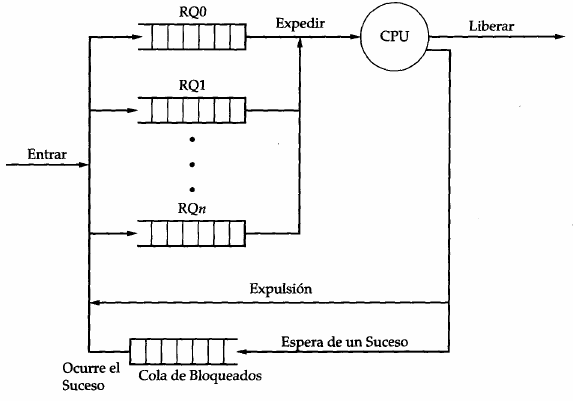
\includegraphics[scale=.9]{img/C06_cpu/prioridades.png}
\caption{Planificación considerando colas de prioridades ($RQ0$ a $RQn$)}
\label{fig:planificacion_prioridades}
\end{figure}

Los casos anteriores (excepto FCFS) son casos particulares de prioridades, por
ejemplo en SJF la prioridad del proceso es su predictor $\tau^p_{n+1}$.

La idea de utilizar prioridades pretende que el sistema pueda ser sensible
frente a las situaciones que en el están ocurriendo, donde un sistema podrá ir
adecuandose a la forma en la que se van ejecutando los procesos.

En general el problema de esta solución es la hambruna, donde procesos con peor
prioridad pueden no ser atendidos nunca.

La solución para la hambruna consiste en utilizar una variante llamada
\textbf{\textit{aging}} (añejamiento), donde cada cierto tiempo se mejora
temporalmente la prioridad de todos los procesos que están en la cola listos.
Ejemplo, cada 10 [ms] hay una interrupción y se mejora la prioridad a todos los
procesos, con esto se espera que después de un tiempo $X$ el proceso alcanzará
la prioridad necesaria para entrar a la CPU. Una vez se concede el acceso a la
CPU y el proceso sale, este retoma su prioridad original.

Otra técnica para evitar la situación de hambruna es el uso de prioridades con
retroalimentación, donde una vez que el proceso ha sido atendido por la CPU al
salir de esta pasará a una cola de menor prioridad. Esto con el objetivo de
permitir que otros procesos puedan entrar a la CPU, ver figura
\ref{fig:planificacion_realimentacion}.

\begin{figure}[htbp]
\centering
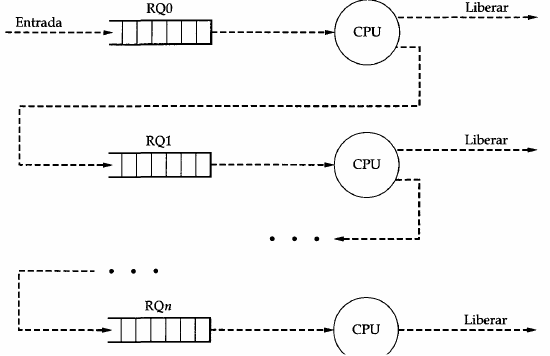
\includegraphics[scale=.9]{img/C06_cpu/realimentacion.png}
\caption{Planificación considerando colas de prioridades con realimentación}
\label{fig:planificacion_realimentacion}
\end{figure}

\subsection{Round Robin}
Se busca minimizar el tiempo de respuesta y es la estrategia de planificación
utilizada hoy en día. Se diseñó específicamente para sistemas de tiempo
compartido, los cuales típicamente son interactivos.

El \textbf{tiempo de respuesta} en sistemas interactivos es el tiempo que
transcurre desde que el usuario inicia una interacción hasta observar el primer
resultado. Si un comando entrega una serie de líneas, el tiempo entre línea y
línea será el tiempo de respuesta.

Psicológicamente se mostró que al usuario le interesa ir viendo resultados, o
sea ir viendo que aparecen líneas avanzando en la pantalla. Un comando que se
demora 10 segundos, pero estuvo entregando durante los 10 segundos respuestas es
mejor, psicológicamente, que un comando que duro 5 segundos, pero durante esos 5
segundos no se entregó ninguna respuesta por la pantalla, sino solo hasta el
final.

En este método de planificación los procesos forman una lista circular y el
\textit{scheduler} da tajadas de tiempo, típicamente de 10 a 100 [ms], a cada
uno de los procesos.

\textbf{¿Cuál es el tamaño de la tajada de tiempo?} Si es muy grande se
parece a FCFS, si es muy pequeña habría un costo excesivo en el cambio de
contexto. Regla empírica, el 80\% de las ráfagas de CPU deben durar menos que el
tiempo de la tajada.

En este tipo de \textit{scheduling} la decisión crítica es \textbf{¿qué hacer
con las ráfagas que llegan?}, ya que cuando la ráfaga llega uno podría proponer:

\begin{enumerate}[i.]

\item Se otorga inmediatamente la CPU a dicho proceso con la tajada de tiempo
completa (de bloqueado a listo), esto tiene sentido porque un proceso que estaba
en estado de espera, el mismo cedió la CPU para ingresar al estado de espera. El
problema, según como sea el \textit{scheduling}, procesos que son intensivos en
lectura escritura podrían causar hambruna a los que son intensivos en CPU.

\item Para evitar la hambruna, se puede adoptar que cuando un proceso pase a
estado de espera, al recibir el recurso, no recibe la tajada completa, sino lo
que le quedaba de tajada. El problema con esto, hay muchos cambios de contexto
si los procesos son intensivos en E/S.

\item Otra variante, para minimizar el cambio de contexto, el proceso se deja
para más adelante ubicándolo al final o al inicio. Cada una con sus problemas,
la primera lo desfavorecería, la segunda podría provocar cierta hambruna en
procesos que son intensivos en CPU.

\end{enumerate}

El debate es ¿cómo minimizar el sobre costo de cambios de contexto dando uso
equitativo de la CPU?

\section{Planificación en Linux}
El \textit{scheduling} en sistemas Unix se realiza utilizando el sistema de
prioridades más el uso de \textit{aging} (para evitar hambruna). En caso de
procesos de misma prioridad se utiliza Round Robin.

Para efectos de planificación los procesos son clasificados en 3 grupos:
\begin{itemize}
\item Procesos batch: sin interacción con el usuario, generalmente en segundo
plano (ej: compiladores, base de datos).
\item Procesos interactivos: interacción continua con los usuarios, deben ser
procesos atendidos rápidamente (ej: editor de textos).
\item Procesos de tiempo real: tiempo corto de respuesta (ej: video, audio,
sensores externos).
\end{itemize}

Es difícil determinar si un proceso es batch o interactivo, por lo cual se
utilizan estadísticas basadas en el comportamiento previo de un proceso para
determinar a que tipo corresponde.

Además los procesos pueden ser clasificados como:

\begin{itemize}
\item Procesos convencionales: interactivos y batch.
\item Procesos no convencionales: tiempo real.
\end{itemize}

``Para poder determinar qué proceso se debe ejecutar a continuación, el
planificador de Linux  busca  en  la lista  no  vacía  con  la prioridad
estática más alta y toma el proceso a la cabeza de dicha lista. La política de
planificación determina para cada proceso, dónde se insertará en la lista de
procesos, con qué prioridad estática y cómo se moverá dentro de esta
lista.''\footnote{Citado textualmente desde man}

Los algoritmos de scheduling encontrados dentro del núcleo Linux son:
\begin{itemize}
\item SCHED\_FIFO: cola estándar para procesos en tiempo real, mientras no haya
un proceso de prioridad mayor el proceso tendrá la CPU.
\item SCHED\_RR: tiempo compartido en tiempo real, asignación justa a procesos
con igual prioridad.
\item SCHED\_OTHER: planificador de tiempo compartido universal.
\item SCHED\_BATCH: para procesos convencionales cuando el procesador esta
``inactivo''.
\end{itemize}

\subsection{Planificación de procesos convencionales}
Para asignar la prioridad se monitorean los procesos y según lo que van haciendo
son favorecidos o penalizados en su prioridad (dependiendo de si han obtenido o
no la CPU). Se distinguen 2 tipos:

\begin{itemize}
\item Estática: asignada inicialmente a un proceso, no responde a los cambios
del sistema (heredada del proceso padre).
\item Tiempo real o dinámica: responde a los cambios del sistema, y al
comportamiento del proceso.
\end{itemize}

Ambas prioridades se mueven entre los valores 100 (mejor prioridad) y 139 (peor
prioridad).

\subsubsection{Prioridad estática}
Para procesos convencionales se utiliza una prioridad estática, que va desde 100
a 139. Esta se verá afectada por el comando \textit{nice} o la llamada a sistema
\textit{setpriority}. Esta prioridad ayudará a determinar el ``quantum'' base
del proceso, de tal forma que:
\begin{itemize}
\item $PE < 120 => quantum = (140 - PE) * 20 [ms]$
\item $PE >= 120 => quantum = (140 - PE) * 5 [ms]$
\end{itemize}

\subsubsection{Prioridad dinámica}
La prioridad dinámica es calculada según el comportamiento del proceso en el
sistema, donde, según como sea este, recibirá un \textit{bonus} para mejorar o
empeorar su prioridad. Al igual que con la prioridad estática su valor va entre
100 y 139. El planificador buscará por esta prioridad al momento de elegir un
proceso para que entre a la CPU.

Se define como: $PD = max (100, min (PE - bonus + 5, 139))$, donde  el bonus es
un valor de 0 a 10, relacionado con el tiempo de \textit{sleep} promedio del
proceso.

Ejemplo: $PD = max (100, min (120 - 5 + 5, 139)) = 120$

El \textbf{tiempo de \textit{sleep}} corresponde a un promedio del tiempo que el
proceso ha pasado durmiendo (sin entrar a la CPU). Este tiempo decrece mientras
un proceso esta corriendo y será como máximo 1000[ms], independientemente del
tiempo real que lleve sin entrar a CPU. El bonus se define utilizando el tiempo
de \textit{sleep} como : $bonus = floor ( tiempo / 100 )$.

Utilizando este tiempo de \textit{bonus} se puede determinar si un proceso es
interactivo o batch utilizando la siguiente fórmula $bonus – 5 >= PE / 4 - 28 =>
interactivo$. Por la fórmula anterior tenemos que un proceso con prioridad
estática \textit{default} (o sea 120) al iniciar no será considerado
interactivo, solo aquellos con una prioridad mejor (o sea 119 o menos). ¿Cuándo
un proceso con prioridad \textit{default} será considerado interactivo?

\subsection{nice}
\textit{nice} permite empeorar (o mejorar) la prioridad estática de un proceso,
esto permitirá ajustar el valor entre 100 y 139, sin embargo para mejorar la
prioridad se requieren privilegios de administrador (usuario \texttt{root}). Lo
anterior ya que la idea original de \textit{nice} era que un usuario fuese
amable (\textit{nice}) con otros al bajar la prioridad de sus procesos.

Los parámetros de la instrucción van de -20 a 19, donde, como ya se mencionó
valores negativos solo puede asignarlos \textit{root}. La nueva prioridad se
calculará como $PE nueva = PE default (120) + nice$.

\subsubsection{Ejemplo}
A continuación se adjunta un ejemplo en C que afecta la prioridad estática de
un proceso. Se sugieren distintas formas de ejecución con diferentes resultados.

\begin{lstlisting}
#include <sys/time.h>
#include <sys/resource.h>
#include <stdlib.h>
#include <stdio.h>
int main (int n, char* args[]) {
    // crear variables para guardar las prioridades
    int prioridadActual, prioridadNueva;
    // determinar prioridad nueva
    if(n==2) prioridadNueva = atoi(args[1]);
    else prioridadNueva = 0;
    // mostrar prioridad con que se llamo al proceso
    prioridadActual = getpriority(PRIO_PROCESS, 0) + 120;
    printf("Prioridad original: %d\n", prioridadActual);
    // cambiar prioridad y mostrarla
    setpriority(PRIO_PROCESS, 0, prioridadNueva);
    prioridadActual = getpriority(PRIO_PROCESS, 0) + 120;
    printf("Prioridad cambiada: %d\n", prioridadActual);
    // salir del programa
    return EXIT_SUCCESS;
}
\end{lstlisting}

\begin{enumerate}[i.]
\item Compilar: \texttt{\$ gcc -Wall prioridad.c -o prioridad}
\item Ejecutar normal: \texttt{\$ ./prioridad}
\item Ejecutar con nice: \texttt{\$ nice -n 10 ./prioridad}
\item Pasar prioridad como parámetro: \texttt{\$ ./prioridad 5}
\item Ejecutar con nice y pasar prioridad como parámetro: \texttt{\$ nice -n 7
./prioridad 3}
\end{enumerate}

¿Qué pasa en el último caso con el valor 3?

\section{Ejercicios y preguntas}
\begin{enumerate}
\item ¿Cuál es la función de las políticas de \textit{scheduling}?
\item ¿Qué tipo jerarquías de planificación existen? Explíquelas.
\item ¿Qué jerarquía es la encargada de elegir el proceso que entrará a la CPU?.
\item ¿Qué condición se debe dar en la ejecución de un proceso para que se
considere que dicha ejecución corresponde a solo una ráfaga de CPU?.
\item ¿Qué es el tiempo de despacho de un proceso?
\item Nombre tres criterios que se pueden utilizar para determinar la estrategia
de planificación a utilizar.
\item ¿Cuál es la diferencia entre políticas de planificación apropiativas y no
apropiativas?
\item ¿FCFS es apropiativo o no apropiativo?
\item ¿Cuál es el gran problema de FCFS?
\item En FCFS, los procesos ¿son todos atendidos?
\item El orden en que llegan las ráfagas en FCFS ¿afectará el tiempo de
despacho? Explique con un ejemplo.
\item ``Primero el trabajo más corto'', ``primero el de menor tiempo restante''
y ``primero el de mayor tasa de respuesta'' ¿son casos particulares de qué
estrategia de planificación?.
\item En SJF, ¿qué es y qué representa el predictor de la ráfaga?.
\item La tasa de respuesta (o \textit{response ratio}) de un proceso, ¿con qué
esta relacionada?.
\item ¿Por qué la estrategia de prioridades presenta hambruna?, explique.
\item ¿Qué técnica se puede utilizar en una planificación con prioridades para
evitar la hambruna?.
\item ¿Por qué es crítico definir de forma correcta la tajada de tiempo en Round
Robin?.
\item ¿Qué tipo de planificación se utiliza en el sistema operativo Linux?.
\item ¿Para que es utilizada la prioridad estática de un proceso en Linux?.
\item ¿Para que es utilizada la prioridad dinámica de un proceso en Linux?.
\item En la prioridad dinámica se utiliza un \textit{bonus} para mejorar o
empeorar esta, ¿de qué depende este \textit{bonus}?.
\item ¿Cuál es la prioridad estática por defecto?.
\item ¿Qué usuarios pueden mejorar la prioridad estática de sus procesos?.
\end{enumerate}

\section{Referencias}
\begin{itemize}
\item Sistemas Operativos, Segunda Edición, Andrew Tanenbaum, Capítulo 2.4.
\item Sistemas Operativos, Quinta Edición, Abraham Silberschatz y Peter Baer
Galvin, Capítulo 5.
\item Sistemas Operativos, Segunda Edición, William Stallings, Capítulo 8.
\end{itemize}


% CAPÍTULO 7: MEMORIA 
%
% Apunte de Sistemas Operativos
% Copyright (C) 2014 Esteban De La Fuente Rubio (esteban[at]delaf.cl)
%
% Permission is granted to copy, distribute and/or modify this document
% under the terms of the GNU Free Documentation License, Version 1.3
% or any later version published by the Free Software Foundation;
% with no Invariant Sections, no Front-Cover Texts, and no Back-Cover Texts.
% A copy of the license is included in the section entitled "GNU
% Free Documentation License".
%
% Link: http://www.gnu.org/copyleft/fdl.html
%

% MEMORIA PRINCIPAL
\chapter{Memoria principal}
\label{memoria_principal}
Todo programa que se quiera ejecutar dentro del sistema, o sea convertirse en un proceso, requerirá como mínimo dos recursos, utilizar la CPU para ejecutar su código y utilizar memoria RAM para almacenar su código y datos. El primer tema fue discutido en el capítulo \ref{planificacion_monoprocesadores}, la asignación de RAM será discutida en este capítulo donde se abordarán los dos temas principales de administración de memoria principal, correspondientes a direcciones virtuales y memoria virtual.

Es importante recalcar que todo proceso que quiera pasar por la CPU requiere estar cargado en memoria principal. Esto implicará que al inicio del proceso el programa debe ser llevado desde el disco (almacenamiento secundario) a la RAM (memoria principal). Adicionalmente es importante recordar las velocidades de operación de los tipos de almacenamientos existentes y sus capacidades se verán afectadas dependiendo de si se trata de discos, ram, cache o registros de cpu, ver figura \ref{fig:memchart}.

\begin{figure}[htbp]
\centering
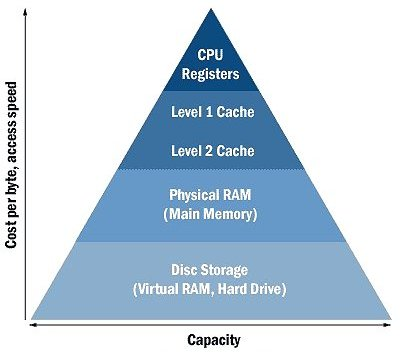
\includegraphics[scale=0.7]{img/C07_memoria/memchart.jpg}
\caption{Tipos de memorias (tiempos, tamaños y costos)}
\label{fig:memchart}
\end{figure}

Finalmente se deberán considerar aspectos relacionados con la protección de la
memoria principal, donde el sistema operativo deberá garantizar que solo los
procesos legítimos puedan hacer uso de cierto espacio de direcciones, evitando
que cualquiera pudiese leer o escribir en cualquier área de la memoria.

\section{Espacio de direcciones}
Originalmente en los ``sistemas operativos'' la administración de la memoria era
bastante simple ya que al existir un solo proceso ejecutándose al mismo tiempo
este se podía copiar completamente a la memoria principal y acceder a los
registros de la misma de forma directa. Sin embargo lo interesante es ver lo que
ocurre en un sistema que utiliza multiprogramación, donde pueden existir
diversos procesos residentes en memoria principal y a todos se les debe asignar
un espacio de memoria para poder ser ejecutados.

La forma más simple de asignar la memoria a diversos procesos es simplemente
tomar todo el programa existente en disco y copiarlo como un solo bloque a la
memoria principal, en cuyo caso para determinar donde se encuentra el proceso
guardado en la memoria basta conocer la dirección inicial, llamada
\textbf{base}, y el tamaño del bloque, llamado \textbf{límite}, en la figura
\ref{fig:baselimite} tenemos una $base=300040$ y un $limite=120900$. Para
movernos dentro del bloque del proceso en la memoria utilizamos un
\textit{offset} o \textbf{desplazamiento}, el cual debe dar como resultado
siempre una dirección dentro del bloque que el proceso tiene asignado, de forma
contraria ocurriría un error de protección o \textit{\textbf{segmentation
fault}}, o sea si la dirección es menor a la base o mayor a la base más el
límite ocurrirá un error, ver figura \ref{fig:segmentation_fault}

\begin{figure}[htbp]
\centering
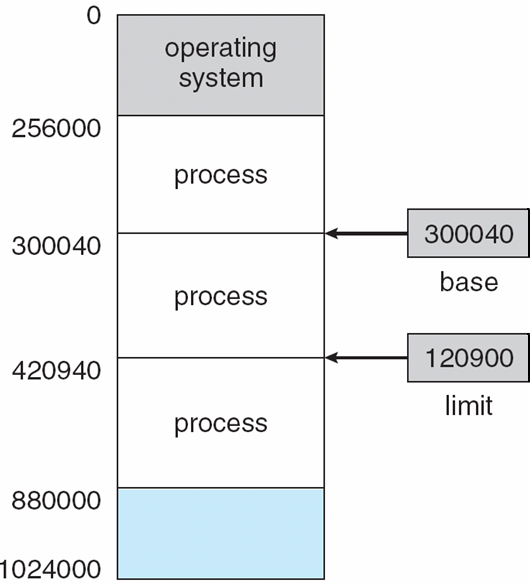
\includegraphics[scale=0.5]{img/C07_memoria/base_limite.png}
\caption{Registro base y límite de un bloque de memoria}
\label{fig:baselimite}
\end{figure}

\begin{figure}[htbp]
\centering
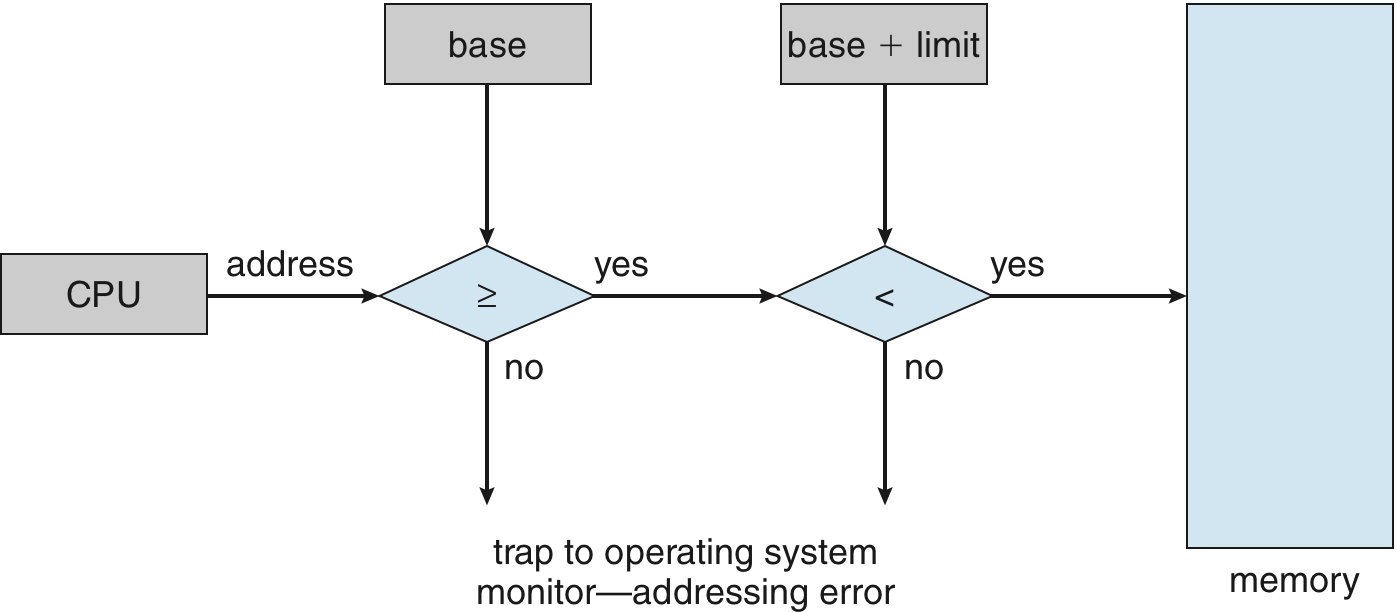
\includegraphics[scale=1]{img/C07_memoria/segmentation_fault.png}
\caption{Protección de memoria, se limita el acceso al bloque del proceso}
\label{fig:segmentation_fault}
\end{figure}

El tipo de asignación descrito anteriormente y mostrado en la figura
\ref{fig:baselimite} corresponde a la \textbf{asignación contigua}, donde todo
el proceso es ubicado en un único bloque de memoria física. De esta forma se
ubicarán diversos procesos en la memoria, pero todos en un único bloque, esto
implica que si no existe espacio contiguo para un proceso deberá sacarse alguno
de los existentes, ver figura \ref{fig:asignacion_contigua}, esto último se
conoce como intercambio y será discutido más adelante.

\begin{figure}[htbp]
\centering
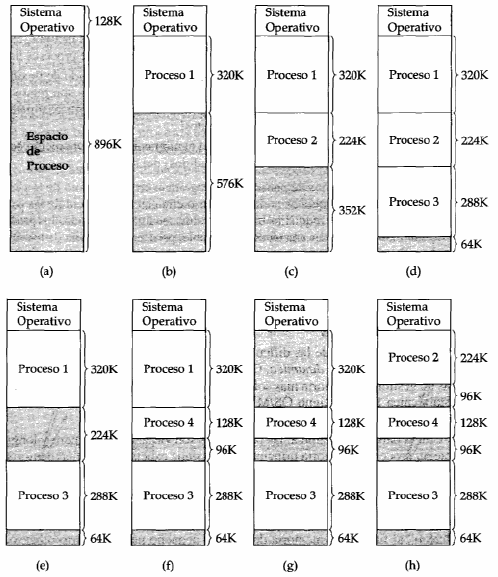
\includegraphics[scale=0.7]{img/C07_memoria/asignacion_contigua.png}
\caption{Asignación contigua}
\label{fig:asignacion_contigua}
\end{figure}

\subsection{Enlace de direcciones}

Una vez se escribe un programa debe ser traducido a código de máquina, ya que el
computador solo entiende direcciones de memoria, no sabe de nombres de variables
ni mucho menos de su semántica. Esto significa que cada una de las variables que
se utilizan dentro del código, y el mismo código, debe ser mapeado a direcciones
de memoria para poder ser utilizado. Lo anterior se conoce como \textbf{enlace
de direcciones} y corresponde al mapeo entre lo que forma el programa (código y
datos) y las direcciones donde se encuentran dichos componentes. Existen
diferentes momentos donde realizar el enlace, cada uno de ellos será mencionado
a continuación y se pueden observar en la figura \ref{fig:memoria_enlaces}.

\begin{figure}[htbp]
\centering
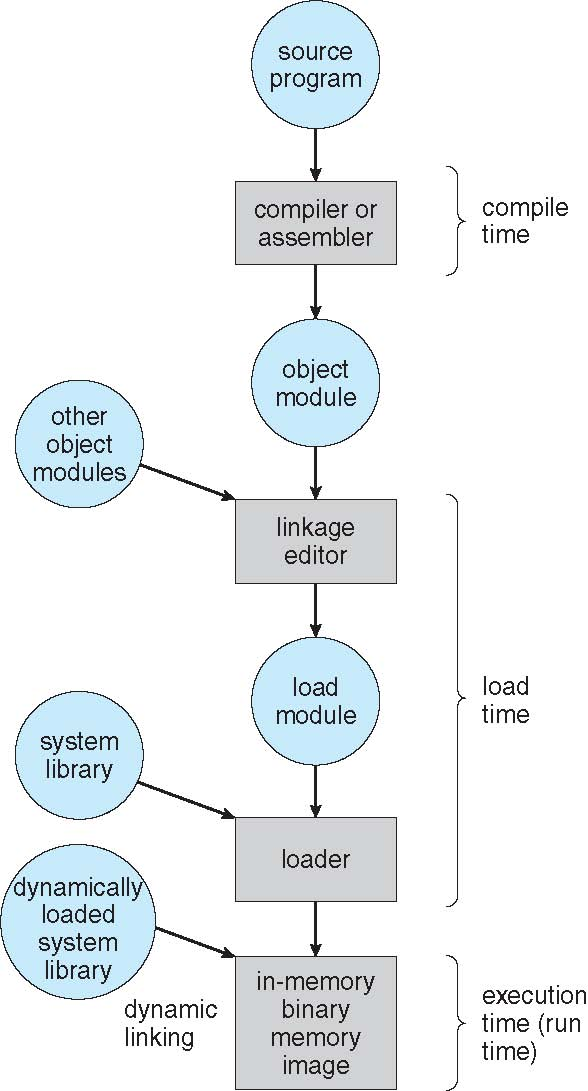
\includegraphics[scale=1]{img/C07_memoria/tipos_enlaces.jpg}
\caption{Tipos de enlaces de direcciones de memoria principal}
\label{fig:memoria_enlaces}
\end{figure}

\subsubsection{Enlace en tiempo de compilación}
Las direcciones de memoria principal son especificadas al momento de compilar el
programa, aquí se indicará donde será cargada cada una de las instrucciones y
variables del código del programa.

Esto tiene diferentes problemas:
\begin{itemize}
	\item El proceso no podrá ser cargado si el bloque que requiere esta
parcialmente o totalmente ocupado.
	\item El proceso no podrá ser movido a otro bloque de memoria una vez
sea cargado.
	\item Se deberán conocer las características físicas de la memoria
principal disponible.
\end{itemize}

Este método tenía sentido en sistemas sin multiprogramación, donde solo un
proceso se encontraba cargado en la ram en todo momento.

\subsubsection{Enlace en tiempo de carga}
En este método el programa generado al compilar no tiene las direcciones de
memoria especificadas, será el sistema operativo el que al cargar el proceso
(estado inicio) asignará las direcciones. De esta forma en diferentes
ejecuciones el programa podría ser ubicado en bloques de memoria diferentes.

El problema aquí seguirá siendo que una vez cargado el programa no podrá ser
movido a otro bloque de memoria. Si por ejemplo se quisiera utilizar intercambio
(al igual que en el caso anterior) el proceso deberá volver al mismo espacio de
direcciones físicas de donde fue sacado, lo cual obviamente representará una
tremenda ineficiencia ya que dicho bloque no podría estar nunca más disponible y
el proceso podría morir de hambruna.

\subsubsection{Enlace en tiempo de ejecución}
En los dos casos anteriores el proceso una vez era cargado en memoria no podía
ser movido a otro bloque, lo que dificultaba que el proceso pudiese crecer (solo
lo haría si hubiesen direcciones contiguas, después de su límite, libres) y
prácticamente imposible hacer intercambio (ya explicado anteriormente).

En este tipo de enlaces el mapeo entre direcciones y los componentes del
programa se realiza en tiempo de ejecución y a medida que el programa va
cambiando (porque necesita crecer o porque es intercambiado) las direcciones de
memoria irán cambiando.

El problema de este método es que la administración de la memoria netamente por
software sería muy complicada y costosa, por las grandes referencias que se
deberían manejar e ir modificando a lo largo de la vida del proceso. Para
solucionar esto y permitir que el enlace pueda ser realizado en tiempo de
ejecución se requiere soporte del hardware, específicamente de la MMU.

\subsection{Direccions virtuales y direcciones físicas}
Uno de los problemas de la multiprogramación es que al existir múltiples
procesos residentes en memoria, si cada proceso utilizará las direcciones de
memoria física para sus enlaces las referencias serían complicadas.

Pensemos por un momento que existe una forma de dividir el programa, de tal
forma que su asignación en memoria no es contigua, el programa se encontraría
dividido por toda la memoria principal, sin embargo para ejecutarse necesita un
espacio de direccionamiento contiguo ya que no se puede cortar un bloque de
datos en un punto para luego continuarlo en otra parte de la memoria física.

Otro escenario interesante donde existen problemas es que sucede si necesitamos
ejecutar un programa que requiere más memoria principal de la que disponemos.

Los casos anteriores se simplifican enormemente al utilizar el concepto de
direcciones virtuales y físicas, donde el espacio de direccionamiento virtual
será contiguo para cada proceso, sin embargo el mapeo de dicho espacio virtual
no será necesariamente contiguo en la memoria física.

Adicionalmente, al ser espacio virtual, se podrían tener más direcciones
virtuales que las físicamente soportadas. Esto tendrá sentido más adelante
cuando se vean paginación y segmentación, sin embargo se puede adelantar que un
proceso solo mantendrá cargado lo que necesita y no todo el código o datos del
programa. Esto permitirá cargar programas más grandes que la memoria principal
disponible mediante el uso de direcciones virtuales.

Este mismo concepto es el requerido para el enlace en tiempo de ejecución, donde
un proceso verá el mismo esquema de direcciones virtuales siempre, pero será la
MMU la que se encargará de actualizar las referencias físicas de dichas
direcciones virtuales. Este proceso es totalmente transparente para el proceso y
no se enterará en caso que hayan cambios o lo muevan entre bloques físicos de
memoria.

\subsection{Unidad de administración de memoria MMU}

La unidad de administración (o gestión) de memoria o MMU (del inglés
\textit{Memory Management Unit}) corresponde a la unidad que permite traducir
direcciones virtuales a direcciones reales de memoria principal. De esta forma
un proceso tiene una vista virtual de la memoria, donde varios procesos podrían
tener visión de una misma dirección virtual, la cual es mapeada a direcciones
reales diferentes.

Procesadores de computadores personales iniciales, 8088 o 68000, no contaban con
MMU, por lo cual al no contar con MMU dichas máquinas no podían correr sistemas
operativos Unix (ya que no había fork lo que implica que no hay shell). Esta
característica (MMU) si estaba disponible en los \textit{mainframes} (desde
fines de los 60s). Con los procesadores 386 (Intel) y 68030 (Motorola) estuvo
disponible una MMU en computadores personales a mediados de los 80s.

Sistemas embebidos, como DVD, lavadoras, etc, generalmente no incluyen MMU, ya
que existen menores posibilidades de caídas en el software. En caso que este se
``caiga'' se tiene que reiniciar el sistema, apagándolo, desenchufando o
presionando el botón de encendido por X\footnote{Típicamente 4 segundos.}
segundos.

\section{Asignación no contigua}
A continuación se discutirán métodos de asignación no contigua de la memoria
principal. Recordar que esto aplica a las direcciones físicas, ya que el espacio
de direcciones virtuales siempre será contiguo.

\subsection{Segmentación}
Este tipo de división ya no se utiliza pero es pedagógicamente interesante ya
que es una forma simple de dividir la memoria. Cada proceso necesita al menos 4
segmentos para funcionar, los cuales corresponden al código, los datos, la pila
y el espacio del sistema.

En la figura \ref{fig:memoria} se puede apreciar la división del espacio de
memoria de un proceso, notar que en esta imagen el espacio de datos se encuentra
separado entre las variables globales y el espacio para solicitud dinámica de
memoria (\textit{malloc}). También notar que hay un espacio para bibliotecas
compartidas, de esto se hablará más adelante y tendrá sentido al ver paginación.

\begin{figure}[htbp]
\centering
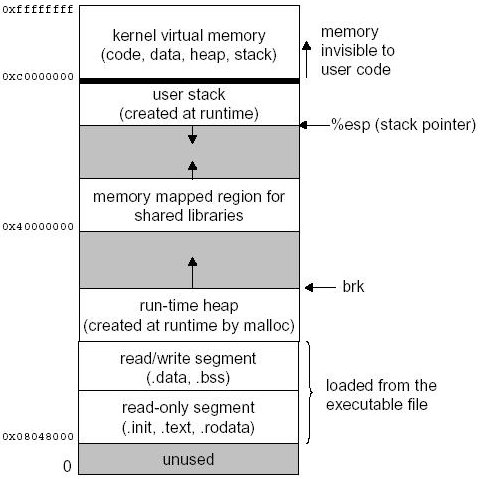
\includegraphics[scale=2]{img/C07_memoria/memoria.png}
\caption{Registro base y límite de un bloque de memoria}
\label{fig:memoria}
\end{figure}

A continuación se describe cada uno de los cuatro segmentos:

\begin{enumerate}[i.]
	\item Código
	\begin{itemize}
		\item Instrucciones binarias del programa.
		\item Solo lectura.
		\item Inicio cercano a la dirección 0, por ejemplo 128 Kb.
	\end{itemize}
	\item Datos
		\begin{itemize}
			\item Variables globales inicializadas.
			\item Variables globales no inicializadas.
			\item heap para malloc y free.
			\item Lectura y escritura.
		\end{itemize}
	\item Pila
	\begin{itemize}
		\item Variables locales.
		\item Información para volver a la rutina que llamo a la
función.
		\item Lectura y escritura.
	\end{itemize}
	\item Sistema
	\begin{itemize}
		\item No se puede leer ni escribir en modo usuario.
		\item Segmento compartido entre todos los procesos.
		\item Inicia en todos los procesos en la misma dirección de
memoria.
	\end{itemize}
\end{enumerate}

Cada uno de los cuatro segmentos será almacenado de forma contigua en la memoria
física, o sea si el programa esta dividido en cuatro segmentos en la memoria
física habrán cuatro segmentos. Se pueden tener los cuatro segmentos separados
en la memoria real, ya que al utilizar direcciones virtuales todo el proceso se
verá continuo en este espacio lógico.

Notar que todos los procesos comparten la memoria correspondiente a la parte de
sistema (núcleo), sin embargo solo pueden acceder a ella en modo sistema, no en
modo usuario.

Entre la pila y el sistema se encuentra una zona de espacio de memoria no
asignada utilizada para crecer al ir solicitando más memoria con
sbrk\footnote{man sbrk}. Por razones históricas existe el \textit{segmentation
fault}, sin embargo actualmente debiese ser \textit{page fault}.

El sistema real, la máquina, tendrá una cierta cantidad de memoria física, por
ejemplo 4 Mb, entonces un proceso verá sus direcciones virtuales (descritas
anteriormente) mapeadas a las direcciones reales en la memoria física
disponible.

La traducción de direcciones virtuales a reales será realizada mediante la tabla
de segmentos, donde existe una tabla por cada proceso (que pertenece a su
contexto). Dependiendo de la implementación de la tabla de segmentos se pueden
guardar diferentes registros (direcciones) todas apuntando a poder obtener la
dirección física en memoria principal a partir de una dirección virtual.

En la figura \ref{fig:tabla_segmentos} se puede observar el proceso de
traducción de una dirección virtual utilizando segmentos a una dirección física.
Importante mencionar que la dirección lógica entregará el segmento al que
corresponde y un desplazamiento dentro de dicho segmento. De esta forma
podríamos tener una dirección lógica dentro del segmento de datos y otra dentro
de la pila, ambas con el mismo desplazamiento. Una vez se tiene el segmento se
busca en la tabla de segmentos si dicho segmento tiene asociada una dirección
base (física) asignada, si lo tiene se suma a su desplazamiento (previa
verificación que este dentro del límite del segmento) y se obtiene la dirección
real en la memoria secundaria.

\begin{figure}[htbp]
\centering
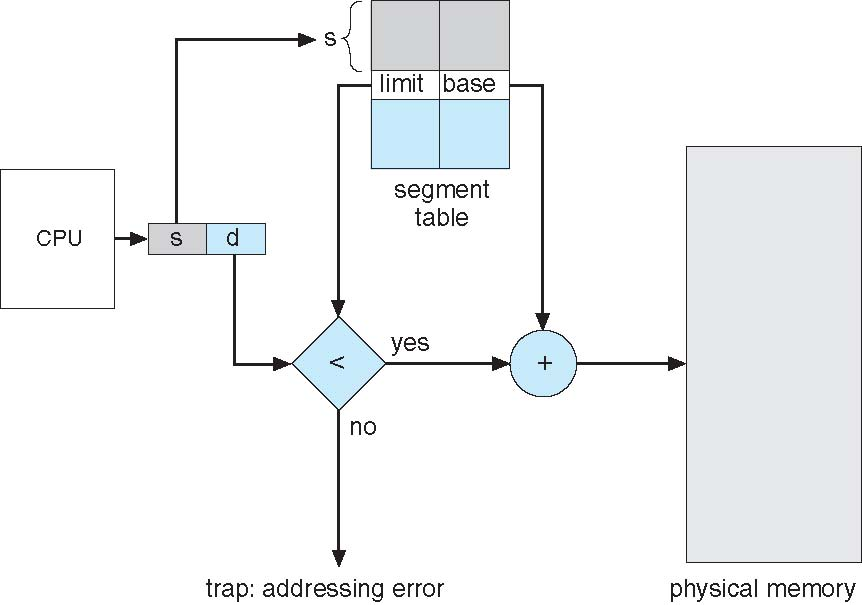
\includegraphics[scale=1]{img/C07_memoria/tabla_segmentos.jpg}
\caption{Traducción de segmentos}
\label{fig:tabla_segmentos}
\end{figure}

Esta traducción se realiza por hardware en la MMU, lo cual toma aproximadamente
un ciclo del reloj. La MMU mantiene la tabla del proceso en ejecución solamente,
ya que sería costoso (para el hardware) mantener todas las tablas.

Al existir un cambio de contexto la tabla de segmentos se almacena en el
descriptor del proceso y se debe cambiar la tabla del proceso saliente por la
del proceso entrante.

\subsubsection{Administración de segmentos}

Se deben crear tres segmentos al crear un proceso (fork), al hacer exec o al
hacer sbrk, importante recordar que el segmento de sistema no se crea en la
memoria principal, ya que dicho segmento es compartido entre todos los sistemas
y corresponde el código y datos del sistema operativo. La destrucción de los
segmentos se realiza cuando el proceso termina.

El núcleo mantiene un \textit{heap} de memoria para segmentos, el cual es
utilizado para los segmentos que se van creando y destruyendo. Esta se
administra de forma similar a como se maneja malloc y free.

Por ejemplo para la administración de los segmentos se puede utilizar una lista
enlazada de pedazos de segmentos disponibles. Esta lista representa trozos de
memoria contigua, en la cual cuando se crea un segmento se debe buscar cual es
el ``mejor'' pedazo para ubicar el segmento del proceso. Cuando se destruye un
segmento se debe devolver a esta lista el espacio liberado, y de ser necesario
unirlo a un segmento contiguo que ya estuviese libre.

El mayor problema es el elegir que segmento entregar, ya que se debe considerar
el tamaño del mismo. Históricamente existen 3 estrategias:

\begin{itemize}
	\item \textbf{First-fit o primer ajuste}: recorrer secuencialmente la
lista desde el inicio hasta encontrar un espacio que alcance para el segmento,
se divide el segmento usando el tamaño preciso y devolviendo lo que no se
ocupará a la lista enlazada. Esto achica trozos disponibles dejando cada vez
tamaños más pequeños libres.
	\item \textbf{Best-fit o mejor ajuste}: busca en toda la lista cual es
el tamaño más cercano  suficiente para el segmento. El problema es que debe
recorrer toda la lista y va dejando pedazos demasiado pequeños cada vez.
	\item \textbf{Worse-fit o peor ajuste}: busca en toda la lista y entrega
el peor caso, es teórico y no se usa.
\end{itemize}

De los anteriores el más eficiente es \textit{first-fit}, ya que
\textit{best-fist} deja muchos segmentos pequeños, tan pequeños que no sirven
para ningún segmento. Adicionalmente se debe recorrer la lista completa cada
vez, lo cual no es bueno.

Una mejora a \textit{first-fit}, quedando como el mejor mecanismo para la
asignación, es el uso de una lista circular. De esta forma no se parte cada vez
del inicio de la lista, sino que se parte desde donde se dejo la última vez .
Esto evita que los pedazos pequeños queden todos al inicio y la búsqueda sea más
rápida, distribuyendo uniformemente los pedazos dentro de la lista.

Las técnicas anteriores producen el problema de \textbf{fragmentación externa},
los métodos anteriores producen pedazos de memoria pequeñas, que no pueden ser
utilizados, sin embargo la suma de estos pedazos pueden servir para atender a un
segmento. Ejemplo, 5 trozos de 1K, se necesita un segmento de 3K, con los 5
trozos no se puede atender al segmento, pero si se pudieran unir si se podría.

Como solución al problema de fragmentación externa existe la
\textbf{compactación}, la cual une los segmentos libres cambiando las
direcciones reales, se deben corregir las tablas de segmentos de los procesos
afectados. Las direcciones virtuales no cambian, por lo cual el proceso de
compactación es transparente para los procesos. El problema de esta solución, es
que se introduce una pausa al momento de ser realizada la compactación por el
tiempo requerido para realizar la copia desde un lado de la memoria principal a
otro, aún así esto es mejor que no poder entregar memoria.

Otra alternativa a la falta de memoria, es el cambio de memoria entre RAM y
disco, mediante el uso de memoria virtual o \textit{swap} lo cual será visto más
adelante.

\subsubsection{Potencial de la segmentación}
Si bien segmentación no es lo que actualmente se utiliza, tiene la ventaja de
ser más sencillo y fácil de implementar.

\begin{enumerate}[i.]

\item \textbf{Incremento del espacio para \textit{heap}.}

Supongamos tenemos un área de datos en un proceso, donde se encuentra su heap.
malloc pide memoria pero no hay, por lo cual es llamado sbrk para aumentar el
tamaño del segmento de datos.

Para implementar la llama a sistema sbrk el núcleo debe:
\begin{enumerate}
	\item Solicitar un segmento más grande.
	\item Copiar el contenido.
	\item Liberar el antiguo segmento.
	\item Actualizar la tabla de segmentos.
\end{enumerate}

Lo que el proceso ve es lo ``mismo'', solo cambia el límite virtual del
segmento, lo cual es natural ya que el proceso está pidiendo memoria. Sin
embargo los cambios de direcciones reales del segmento, lo cual si cambio, no es
visible por el proceso.

Se puede utilizar una optimización que no copie, realloc permite hacer esto
extendiendo el segmento a un trozo contiguo libre. De hecho malloc
automáticamente utilizará sbrk o realloc dependiendo de la situación, sin
embargo si no hay un segmento contiguo libre necesariamente se debe copiar hacia
otro lado ya que en segmentación cada segmento se debe encontrar de forma
contigua en la memoria física.

\item \textbf{Desborde de la pila}

Esto ocurre automáticamente al ir llamando funciones (por ejemplo de forma
recursiva). Para evitar que se produzca un \textit{overflow}, el núcleo pide más
memoria de forma transparente para el proceso más memoria. Esto se hará
adivinando cuando se podría requerir más memoria para la pila, y el núcleo
interrumpirá al proceso (sin que este se entere) y la aumentará.

En caso que ocurriese un desborde de la pila y se tratase de acceder a un área
que no ha sido asignada ocurrirá un \textit{segmentation fault}. Donde si el
proceso no atrapa la señal del \textit{segmentation fault}, el núcleo enviará
una señal al proceso padre indicando el error y será el padre (la shell) quien
imprimirá el mensaje.

\item \textbf{Implementación de fork}

\begin{verbatim}
int pid = fork();
if (pid==0) {
  // hijo
} else {
  // padre
}
\end{verbatim}

Como el segmento de código es de solo lectura y común para todos los hijos, se
puede mapear para todos los hijos el mismo trozo físico en la memoria real para
dicho segmento. Esto evita tener que copiar el código y ahorra memoria
principal.

Si un proceso hace fork y hay una variable global que es modificada por el hijo,
el padre no verá este cambio, ya que los procesos no comparten memoria o sea son
procesos pesados. Cada proceso tendrá su propio segmento de datos.

\item \textbf{Swapping}

Cuando la memoria escasea el scheduler de mediano plazo lleva procesos completos
a disco. El estado del proceso cambia a SWAPPED y se guardan copias al bit de
los segmentos que se envían a disco. En algún momento se llevarán a disco otros
procesos y se restaurará este, lo más probable en otra dirección física de
memoria, esto sigue siendo transparente para el proceso.

Esto es crítico en procesos interactivos. Sigue siendo mejor a no tener memoria
y no poder atender a nuevos o tener que matar procesos. Se trata de evitar
llevar procesos interactivos a disco.

\end{enumerate}

\subsection{Paginación}
La paginación corresponde a otro método de asignación de memoria física no
contigua, el cual es el actualmente utilizado. Básicamente es muy similar a la
segmentación, sin embargo aquí la memoria no se divide por segmentos si no que
se divide en páginas.

Específicamente es el proceso el que se divide en páginas de igual tamaño cada
una de ellas y la memoria principal se divide en marcos de igual tamaño que las
páginas. De esta forma cuando se crea un proceso y se copia el código más los
datos estos son llevados a marcos en la memoria principal los cuales no
necesariamente estarán contiguos. Al igual que en segmentación, desde el punto
de vista de direcciones lógicas las páginas están contiguas.

La paginación no presenta el problema de fragmentación externa, por lo cual no
requiere compactación. Sin embargo el problema que aparece es el de la
\textbf{fragmentación interna}, ya que los marcos al ser de tamaño fijo puede
ocurrir que una página de un proceso no complete el marco quedando espacio libre
dentro de dicho marco. Este espacio puede ser utilizado para crecer
eventualmente, pero de no ser utilizado será desperdiciado.

En la figura \ref{fig:paginacion_varios_procesos} se puede observar como tres
procesos han sido divididos en páginas del mismo tamaño, la memoria principal ha
sido dividida en marcos del mismo tamaño que las páginas. Cada página se ubica
en un marco dentro de la memoria principal. Es la tabla de páginas la que dice
que página se encuentra en que marco.

\begin{figure}[htbp]
\centering
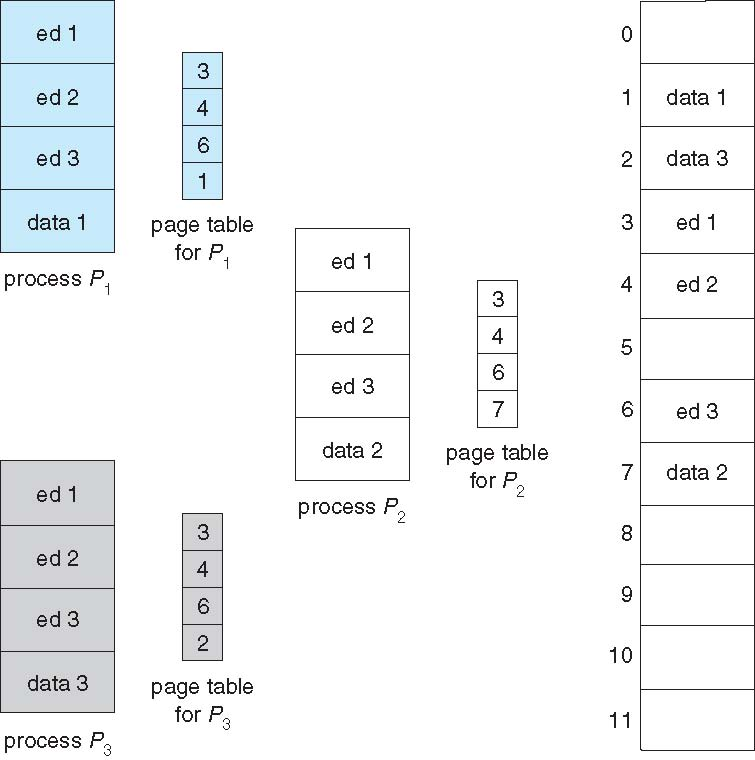
\includegraphics[scale=1]{img/C07_memoria/paginacion_varios_procesos.jpg}
\caption{Ejemplo de paginación con 3 procesos}
\label{fig:paginacion_varios_procesos}
\end{figure}

\subsubsection{Carga dinámica}
El hecho de tener ahora páginas permitirá llevar a la memoria principal partes
del código o datos del programa, no teniendo que llevar todo el código (como
ocurría con segmentación) de esta forma se cargarán bajo demanda las páginas del
proceso y si existen algunas que nunca se lleguen a utilizar entonces nunca
serán cargadas en la memoria principal.

Esto lo que busca es reducir el espacio, específicamente marcos, utilizados por
un proceso en la memoria principal, cargando solo lo que es necesario.

Para utilizar la carga dinámica el sistema operativo deberá vaciar la memoria
cache L1 (de nivel 1) para que se produzcan los fallos de página del proceso que
está en ejecución cada vez que ocurra un cambio de contexto. La acción de vaciar
la caché es la que finalmente representa gran parte del costo del cambio de
contexto.

\subsubsection{Enlace de bibliotecas}
Cuando un programa requiere hacer uso de alguna biblioteca que esta en el
sistema existen dos alternativas para el enlace de las mismas, un enlace
estático y otro dinámico.

En el \textbf{enlace estático} las bibliotecas son agregadas al ejecutable al
momento de la compilación. Esto implica un mayor tamaño en el programa
resultante y eventualmente una mayor cantidad de páginas que cargar en memoria
cuando el programa se ejecute. Esto tiene además el problema que se repetirán
páginas de la biblioteca entre varios procesos que la usen y la tengan enlazada
de forma estática en su código.

En el \textbf{enlace dinámico} al momento de compilar solo se deja una
referencia a las bibliotecas, las cuales deberán ser cargadas por el sistema al
momento de la ejecución del programa pero en un espacio diferente al código del
programa. De esta forma se podrán compartir varias bibliotecas entre varios
procesos en ejecución, en el fondo se compartirán las páginas cargadas
correspondientes a dichas bibliotecas. Si la página requerida no esta cargada
cuando la solicita un proceso P1 se cargará en un marco M1, cuando un proceso P2
requiera la misma página de la biblioteca no se volverá a cargar si no que se
hará referencia al marco M1 ya cargado. Este espacio para cargar bibliotecas
compartidos puede apreciarse en la figura \ref{fig:biblioteca_compartida}.

\begin{figure}[htbp]
\centering
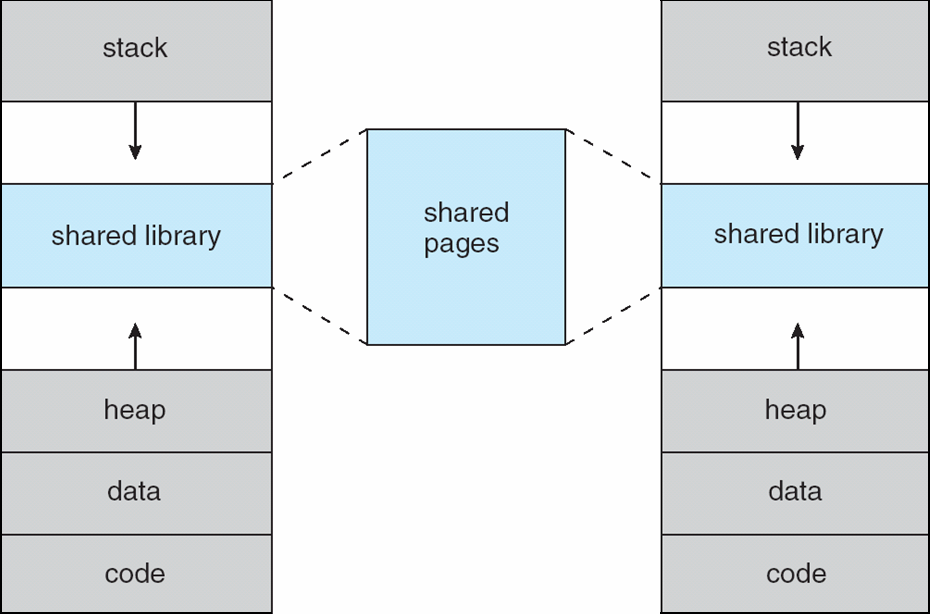
\includegraphics[scale=0.45]{img/C07_memoria/biblioteca_compartida.png}
\caption{Biblioteca compartida entre dos procesos}
\label{fig:biblioteca_compartida}
\end{figure}

Uno de los problemas con el enlace de bibliotecas de forma dinámica es el uso de
variables globales en las bibliotecas. Por lo cual si se esta desarrollando un
software con múltiples hebras no se deberán utilizar bibliotecas que no se han
desarrollado para ser utilizadas en procesos ligeros, ya que pueden aparecer
problemas de \textit{dataraces}.

\subsubsection{Procesos semi-pesados}

Adicionalmente a la idea de bibliotecas compartidas, se pueden tener áreas de
datos compartidas entre procesos. Hasta ahora se habían visto procesos livianos
y procesos pesados. Un proceso semi-pesado corresponde a un proceso que puede
compartir ciertas áreas de memoria con otro proceso.

Supongamos un proceso pesado con Código (C), Datos (D) y Pila (P). Un proceso
semi-pesado podría corresponder al proceso pesado anterior (C, D y P) más un
área para datos (D') que es compartida con otros procesos.

Existen funciones que permiten retornar puntos a espacios de memoria compartida,
como por ejemplo \textit{mmap}.

\subsubsection{Implementación tabla de páginas}

Las tablas de páginas son considerablemente más grandes comparadas con las
tablas de segmentos, esto ya que un programa al ser dividido en páginas por lo
general contendrá más páginas que si fuese dividido en segmentos. Por lo
anterior las tablas de páginas no pueden ser almacenadas completamente en la
MMU, y deben ser mantenidas en la memoria principal.

La situación explicada anteriormente implica que por cada acceso ``útil'' a la
memoria principal se requiere un acceso para buscar la tabla de páginas (para
saber donde está lo solicitado) y otro para acceder a lo solicitado. Este doble
acceso para llegar a la memoria principal significa tiempos mayores de acceso a
los datos requeridos.

Como solución al problema de doble acceso se utiliza \textit{TLB}
(\textit{translation lookaside buffer}), lo cual es un \textit{buffer} para la
tabla de páginas. Por lo cual cuando se hacen consultas primero se revisa en la
\textit{TLB} por la página solicitada, y solo si no está ahí, se va a la memoria
principal por ella.

\subsubsection{Traducción de páginas}

La traducción de páginas corresponde a un proceso similar al de la traducción de
segmentos, de esta también se encarga la MMU. La dirección lógica en este caso
entregará el número de página del proceso y el desplazamiento dentro de la
página. Por ejemplo en un sistema con direcciones de 32 bits se podrían utilizar
20 bits para la página (y marco) y 12 bits para el desplazamiento.

En la figura \ref{fig:tabla_paginas} se observa el proceso de traducción, donde
una vez obtenida la página y el desplazamiento se busca en la tabla de páginas
el marco correspondiente a dicha página. En caso que la página no estuviese
cargada en un marco en la memoria ocurrirá un fallo de página y la página deberá
ser traída desde el disco, si la página no existe o el desplazamiento esta fuera
de rango se produce un \textit{segmentation fault}. Una vez se tiene el marco y
se sabe que el desplazamiento es válido se va a la memoria principal con la
dirección física.

\begin{figure}[htbp]
\centering
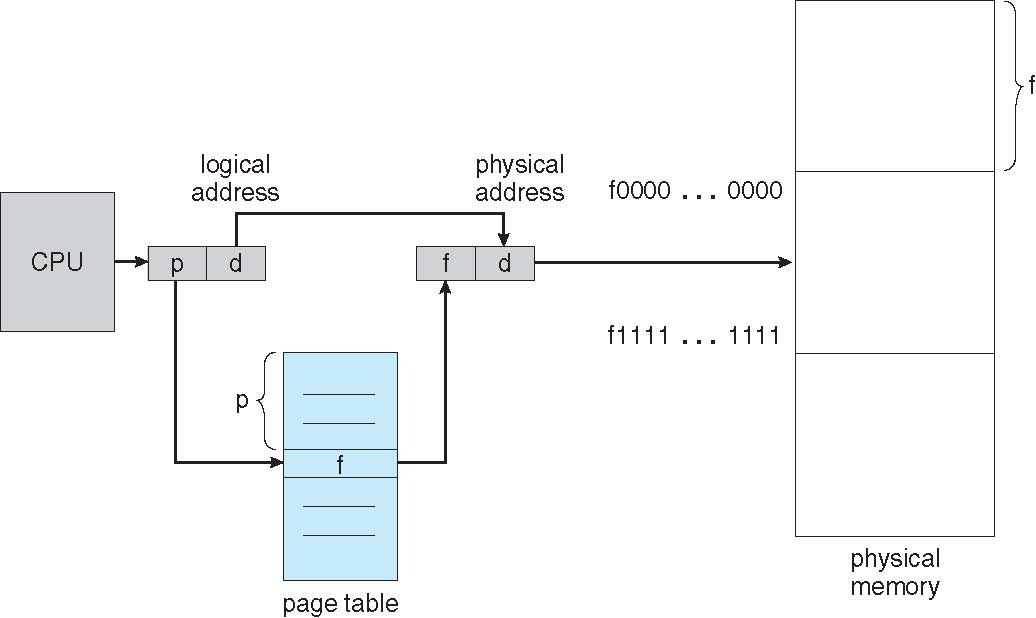
\includegraphics[scale=.9]{img/C07_memoria/tabla_paginas.jpg}
\caption{Traducción de páginas}
\label{fig:tabla_paginas}
\end{figure}

\subsubsection{\textit{Copy on write}}

El objetivo de \textit{copy on write} es hacer un \textit{fork} más eficiente,
donde las páginas serán copiadas en la memoria principal si y solo si son
modificadas. Mientras no sean modificadas las páginas seguirán estando
compartidas entre el padre y el hijo.

En la implementación cuando se realiza \textit{fork} de un proceso las páginas
no son copiadas si no que son marcadas como solo lectura y además se indica que
cuando se quieran escribir primero se deberán copiar. Para esto se utilizarán
campos de los atributos de las páginas para indicar que se debe copiar la página
cuando uno de los procesos (padre o hijo) la desee modificar.

Cada vez que se quiera hacer una modificación se producirá una interrupción que
verificará si la página puede ser escrita, si no lo es se verificará si existe
un bit que indique que se debe copiar, si existe se copiara y luego se
modificará. Si muchos procesos quisieran modificar muchas páginas se producirán
muchas interrupciones, para evitar esto se puede utilizar una heurística que
determine que si se han copiado X páginas a la siguiente interrupción se copien
todas las páginas del proceso a un nuevo espacio, asumiendo que seguirán
ocurriendo interrupciones.

Este método también es conocido como duplicación perezosa de las páginas o copia
bajo demanda.

\subsubsection{Tablas de páginas de dos niveles}

Estos ejemplos son para x86 (32 bits), para procesadores de 64 bits existen
tablas de páginas de 3 niveles asociadas con procesadores de 64 bits.

Para el caso de 32 bits, la dirección de memoria virtual se dividirá en 2
partes. Donde la primera parte a su vez se divide en un bloque \textit{b} (10
bits) y página \textit{p} (10 bits). La segunda parte es el desplazamiento
\textit{d} (12 bits).

En 32 bits el tamaño máximo de memoria que se puede direccionar son 4G, en este
caso la memoria es dividida en 1024 bloques, entonces cada bloque es de 4M. Y
cada bloque es dividido en 1024 páginas, entonces cada página es de 4K.

Existe un directorio de bloques que indica para cada bloque:

\begin{itemize}
	\item \textbf{b}: el bloque.
	\item \textbf{t}: utilizado para entregar la dirección de una tabla de
páginas asociada al bloque \textit{b} (dirección de 10 bits).
	\item \textbf{Atributos}: similares a los de las páginas, pero valido
para todo el bloque (o sea para todas las páginas).
\end{itemize}

Con lo anterior se construye una nueva dirección, formada por $t+p$, que entrega
un puntero directo a la entrada en la tabla de página \textit{t} del bloque
\textit{b}. Con este puntero a la entrada y \textit{p} se puede construir la
dirección real de la página, ya que la entrada de la tabla de páginas (apuntada
por \textit{t}) contiene el marco \textit{m} al cual se le suma \textit{d},
obteniendo la dirección física.

La idea de usar estas dos tablas (por eso se llama tabla de páginas en dos
niveles), es que la mayoría de los procesos requieren menos de 4M. Donde un
proceso ocupará 1 bloque para su código y datos y otro bloque para la pila.
Todas los otros bloques se encontrarán inválidos (no asignados). El espacio que
queda en el bloque es dejado para crecimiento futuro.

El sobre-costo para un típico proceso (menor a 4M) es:
\begin{itemize}
	\item Una tabla para código más datos.
	\item Una tabla para la pila.
	\item Un directorio para manejar los bloques.
\end{itemize}

Tanto el directorio como la tabla de páginas requieren (cada una) 4K, ya que
cada entrada ocupa 32 bits. Por lo cual un proceso menor a 4M requerirá 12K para
manejar su memoria principal. Sobre-costo es muy bajo, menor al 1\% (lo que se
requiere \textit{versus} lo que se podrá direccionar).

Cuando se requiere más memoria, llamando a \textit{sbrk}, se entregarán páginas
dentro del mismo bloque de memoria ya asignado, una vez el bloque se llena se
van pidiendo nuevos bloques de memoria.

Cuando los datos llegan a la dirección de la pila, significa que no hay más
espacio que asignar y \textit{malloc} retornará \textit{NULL} y el proceso no
podrá continuar, asumiendo que terminará cuando \textit{malloc} retorne
\textit{NULL}.

\subsubsection{Tablas de páginas de tres niveles}

Los directorios se referencian de a 4G (o sea se agregan 10 bits más a la
dirección virtual), donde existe otra tabla (tercer nivel) que administra estos
directorios.

En sistemas de 64 bits, se dispone de 64 bits para la dirección, sin embargo
direcciones de 64 bits permitirían referenciar mucha más memoria de la que
actualmente se encuentra disponible. Por lo anterior, de los 64 bits solo se
usan 10 bits más, o sea 42 bits de los 64. Arquitecturas futuras deberán
considerar utilizar más de 42 bits para poder referenciar más memoria.

El problema con este esquema, es que se requieren 3 accesos a memoria para
llegar a la memoria física requerida. Para solucionar esto aquí entra la TLB que
almacena la tabla de páginas y el directorio.

Hoy en día los sistemas operativos modernos asignan bloques completos de memoria
cuando un proceso lo solicita, no páginas. O sea, ya sea que requiera 10K o 3M
se le asignarán 4M. La asignación de páginas de forma individual esta reservada
para actividades especiales, como las del núcleo.

\section{Memoria virtual}
La memoria virtual utiliza espacio de la memoria secundaria (disco) para
almacenar temporalmente los procesos que por algún motivo han sido enviados
fuera de la memoria principal por el planificador de mediano plazo.

El esquema de memoria virtual es utilizado con las páginas, no se llevan bloques
completos a disco solo páginas de dichos bloques. Se podría utilizar este
esquema en segmentación, o en bloques, pero sería muy costoso porque el acceso a
disco es lento. Se hablará de memoria virtual con páginas por ser el esquema
utilizado en los sistemas operativos modernos.

A la tabla de páginas se le agregará un \textbf{bit de validez} (o invalidez,
dependiendo de la implementación), que indicará si la página está o no en
memoria principal. Cuando la página solicitada no se encuentra en un marco se
produce un \textbf{fallo de página} (o \textit{page fault}), indicado por su bit
de invalidez en la tabla de páginas, el sistema operativo captura esto y si
determina que la página esta en el disco procede a llevarla a un marco libre.
Una vez la página ha sido copiada a un marco en la memoria principal, la página
es marcada como válida en la tabla de páginas y se reinicia el proceso desde el
punto donde requería acceder a la página que se cargó. Este proceso puede ser
apreciado en la figura \ref{fig:fallo_pagina} y es importante mencionar que es
totalmente transparente para el proceso.

\begin{figure}[htbp]
\centering
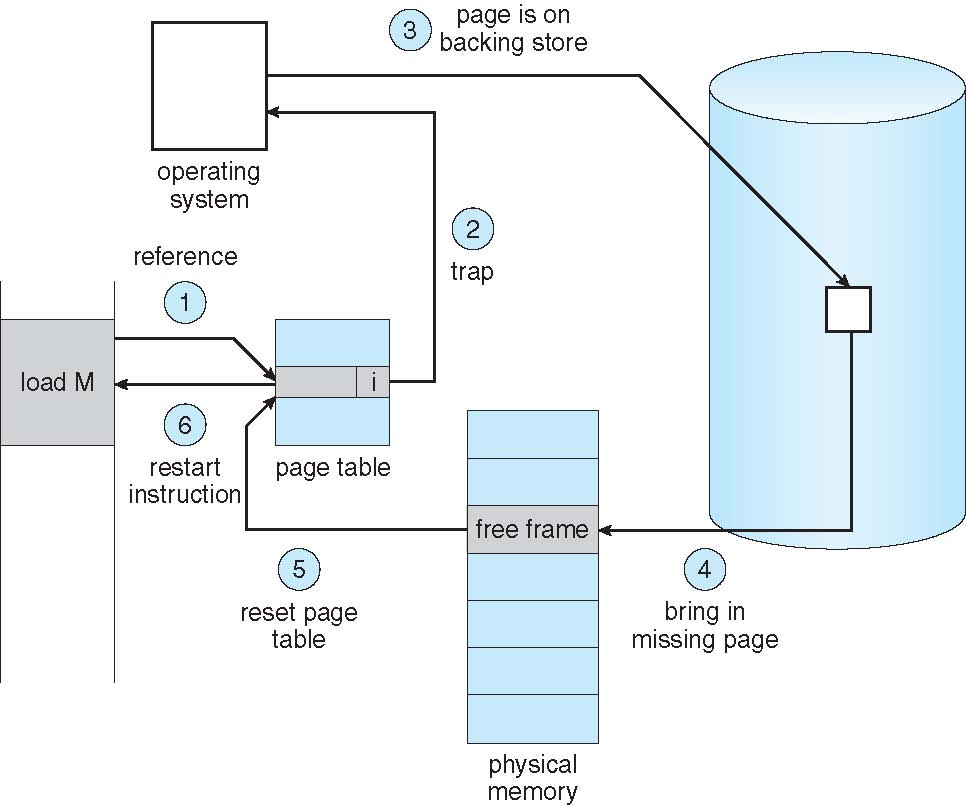
\includegraphics[scale=1]{img/C07_memoria/fallo_pagina.jpg}
\caption{Proceso que ocurre al existir un fallo de página}
\label{fig:fallo_pagina}
\end{figure}

El proceso de \textbf{intercambio} ocurre cuando es detectada una página
inválida y está se encuentra en el disco, pero no hay marco libre en la memoria
principal para ubicarla. Es en este punto donde ocurre lo descrito en la figura
\ref{fig:intercambio}, donde primero se debe llevar a la ``víctima'' desde el
marco en la memoria principal al disco, marcar su página como inválida, luego
llevar la página requerida del disco al marco liberado y marcar esta última
página como ahora válida. Luego se continúa la ejecución con la página cargada
en un marco.

\begin{figure}[htbp]
\centering
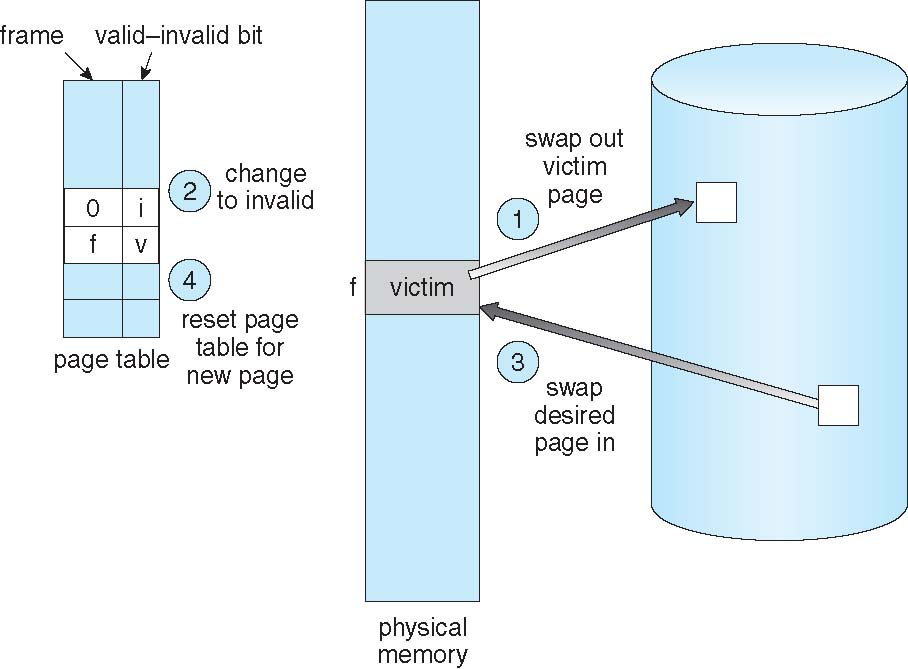
\includegraphics[scale=1]{img/C07_memoria/intercambio.jpg}
\caption{Proceso de intercambio de páginas}
\label{fig:intercambio}
\end{figure}

Un uso lógico de la memoria virtual es cuando el sistema no dispone de más
memoria principal para la creación de nuevos procesos. Adicionalmente el uso de
memoria virtual permitirá disponer en el sistema de un espacio de
direccionamiento virtual mayor al real para los procesos, ya que a pesar de no
tener marcos para todas las páginas del proceso este podría tener aquellas
páginas que no este utilizando en la memoria virtual y solo traerlas a principal
cuando las necesite usar.

\subsection{Algoritmos de reemplazo de páginas}
Para el proceso de intercambio lo crucial es decidir a quién se sacará de la
memoria principal para ser llevado a disco. En estricto rigor se debe determinar
la página que será sacada desde la memoria principal. Para esto existen diversos
algoritmos los cuales serán mencionados a continuación, la idea es encontrar un
algoritmo que en el sistema genere la menor cantidad de fallos de páginas. Lo
último porque el proceso de intercambio es lento ya que implica acceso al
almacenamiento secundario.

En cualquiera de los algoritmos se puede utilizar una optimización que implica
el uso de un \textbf{bit de modificación} (o \textbf{bit dirty}) en la tabla de páginas, este indicará
si la página (que ya esta en disco) fue modificada al estar en la memoria
principal (en un marco). Si fue modificada se copia a la memoria virtual al
existir el intercambio, sin embargo si no fue modificada no se copia, con esto
se reducen los tiempos que dura el fallo de página.

El objetivo de estos algoritmos es ser capaz de elegir una página que será usada
en el futuro más lejano, sin embargo determinar esto es imposible ya que no se
sabe que pasará en el futuro. Sin embargo se puede usar la historia pasada para
poder determinar que páginas podrían usarse en el futuro más lejano. De esta
forma se asumirá, por ejemplo, que una página que no se ha utilizado en el
último minuto no se usará hasta al menos dentro de otro minuto más.

El \textbf{tiempo de acceso efectivo} corresponde al tiempo real que tomará
acceder a la memoria principal si existe un fallo de página. Se define como
$T_{ef} = (1-r) * t_M+r*t_p$, donde:

\begin{itemize}
	\item $t_M$ es el tiempo de acceso a memoria física, por ejemplo 60 ms.
	\item $t_p$ es el tiempo de reemplazo de la página, por ejemplo 12 ms.
	\item $r$ es la tasa de fallos de página.
\end{itemize}

%Si $T_{ef}$ es 10\% superior a $t_M$ se requiere que r = 1 / 2000000.

\subsubsection{Ideal: ``oráculo''}

La estrategia ideal sería consultar el ``oráculo'' y se lleva a disco la página
que permanecerá más tiempo sin ser usada. Lamentablemente esto no se puede
implementar, ya que no se puede ver el futuro. Sin embargo sirve como
referencia.

Ejemplo:
\begin{itemize}
	\item Marcos: 3.
	\item Páginas: 8.
	\item Cadena de referencia: 7,0,1,2,0,3,0,4,2,3,0,3,0,3,2,1,2,0,1,7,0,1
\end{itemize}

¿Cuantos fallos de página generará la cadena de referencia indicada?
% 7, verificar :P

\subsubsection{FIFO}
En este caso se van ubicando las páginas en la memoria en el mismo orden que son
referenciadas, la más ``antigua'' será la que se elegirá como ``víctima'' para
ser sacada en caso de requerir un marco libre. Esta estrategia puede ser
considerada como la peor, sin embargo será las más simple de implementar.

Ejemplo:
\begin{itemize}
	\item Marcos: 3.
	\item Páginas: 8.
	\item Cadena de referencia: 7,0,1,2,0,3,0,4,2,3,0,3,0,3,2,1,2,0,1,7,0,1
\end{itemize}

Luego de la ejecución total del proceso, o sea, cuando se haya procesado toda la
cadena de referencia de páginas habrán ocurrido un total de 15 fallos de
páginas, ver figura \ref{fig:swap_fifo}. Sin embargo la cantidad de fallos de
página dependerá de las solicitudes de páginas, esto significa que con otra
cadena de referencia de memoria podrían haber más o menos fallos de página.

\begin{figure}[htbp]
\centering
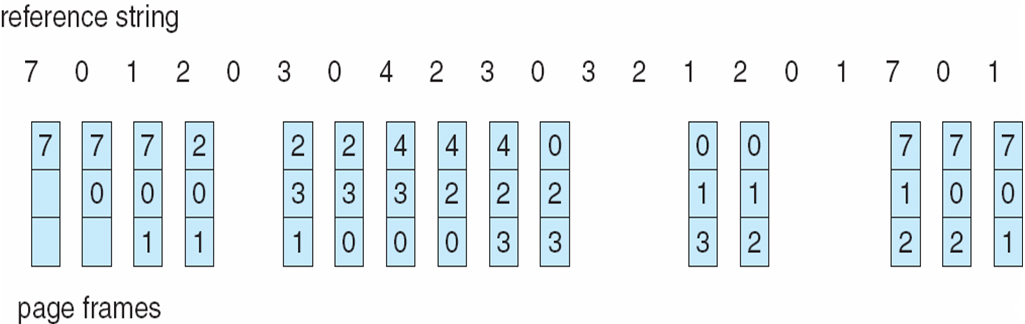
\includegraphics[scale=0.55]{img/C07_memoria/swap_fifo.png}
\caption{Ejemplo de intercambio con algoritmo FIFO}
\label{fig:swap_fifo}
\end{figure}

\subsubsection{LRU}
En este caso la página que es reemplazada es aquella que no ha sido usada en el
último tiempo (\textit{Least Recently Used}), o dicho de otra forma aquella que
fue usada hace más tiempo. Para esto se debe llevar por cada página una
asociación con el tiempo de la última vez que la página fue referenciada.

Implementación:
\begin{enumerate}[a)]
	\item \textbf{Con un contador}: cada entrada de página en la tabla de
páginas tiene un contador, cada vez que la página es referenciada el reloj es
copiado al contador. Cuando una página necesita ser cambiada se mira el contador
y se busca el valor más pequeño. Este método es sencillo de implementar pero
tiene el problema de requerir buscar en toda la tabla de páginas para encontrar
la usada hace mas tiempo, por lo cual resulta muy ineficiente y cara de
implementar. En la práctica no es utilizada.
	\item \textbf{Con una pila}: se mantiene una pila con los números de
página del sistema, cada vez que una página es referenciada se mueve al tope de
la pila. Por lo cual cuando se requiere una página para intercambiar se saca
aquella que esta más abajo en la pila.
\end{enumerate}

\subsubsection{Second chance o estrategia del reloj}
Esta es una aproximación de LRU donde se elige una página que lleve bastante
tiempo sin ser utilizada. Se podría cometer un error y no sacar la que lleve más
tiempo sin ser usada, pero esto es una aproximación que busca aumentar la
velocidad.

El núcleo coloca el bit ``r'' o \textbf{bit de referencia} en 0. Si la página es
referenciada el hardware del procesador (la MMU) coloca el bit ``r'' en 1 cuando
la página se usa. El sobre costo en esto es muy bajo, ya que solo implica ir a
la tabla de página y cambiar un bit. Este cambio se realiza en la TLB, por lo
cual cada cierto tiempo se deberá actualizar el bit en la memoria principal,
pero no es común tener que actualizar de la TLB a la memoria principal.

La página se puede llevar a disco cuando ``r'' permanece en 0 por ``suficiente''
tiempo. ¿Cómo se considera el tiempo? Para esto se utiliza una lista circular
donde cada vez que se quiere sacar una página de la memoria principal se
consulta el bit ``r'', si es 1 la página es dejada en memoria principal (dando
una segunda oportunidad) y su bit es puesto a 0, se continúa así hasta encontrar
una página con su bit de referencia en 0. Se marca el bit de referencia en 1
cada vez que la página es referenciada y se parte revisando a contar de la
página que se cambio la vez anterior.

En la figura \ref{fig:swap_secondchance} se puede apreciar el funcionamiento del
algoritmo, al lado izquierdo desde donde se inicia la búsqueda y al lado derecho
el estado final de los bits de referencia y la ``víctima'' que fue elegida.

\begin{figure}[htbp]
\centering
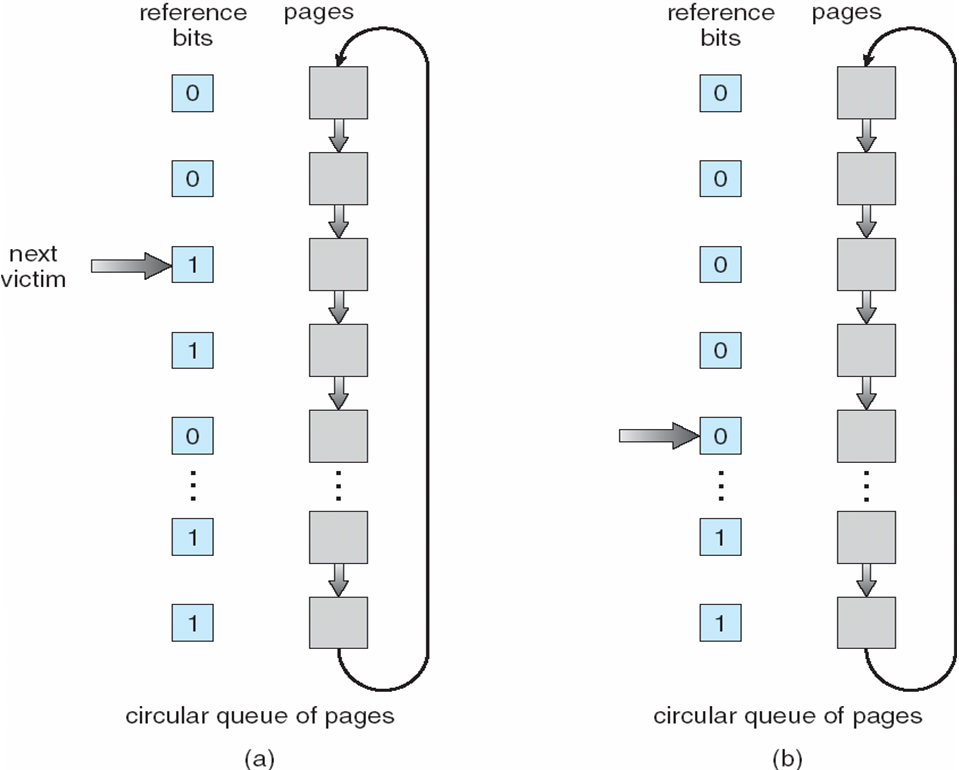
\includegraphics[scale=0.6]{img/C07_memoria/second_chance.png}
\caption{Ejemplo de intercambio con algoritmo Second Chance}
\label{fig:swap_secondchance}
\end{figure}

Esta estrategia es utilizada hoy en día, su seudo código se muestra a continuación:

\begin{verbatim}
while (bitR(cursor())==1) {
  bitR(cursor()) = 0
  avanzarCursor()
}
reemplazarCursor()
AvanzarCursor
\end{verbatim}

Si todas las páginas tienen su bit de referencia \textit{r} en 1 se deberá dar la vuelta completa poniendo los bits en 0 hasta volver a la primera página revisada la cual ahora tendrá el bit en 0 y se escogerá. Esto es una situación anómala ya que en estricto rigor no se está determinando lo esperado, ya que todas estaban en iguales condiciones y se terminó sacando la primera consultada. Se da cuando el tiempo en que se demora en dar la vuelta a la lista es muy grande, sin embargo en la práctica es muy poco probable que ocurra y no es considerado como un problema real.

Un problema real es el \textbf{thrashing}, que corresponde a la situación cuando la tasa de fallos de páginas es muy alta. Esto ocurre cuando ocurren fallos de páginas muy seguidos, el cursor avanza muy rápido y los discos al ser lentos (tiempo de acceso alrededor de 10 ms) se podrían atender aproximadamente 100 fallos de página por segundo. En esta situación el sistema operativo trabajará llevando procesos de disco a RAM y de RAM a disco, pero no se hará trabajo útil. La CPU pasa el 99\% del tiempo ociosa y el disco de \textit{paging} pasa el 100\% del tiempo ocupado, lo anterior significa que los procesos no avanzan. Recuperarse de esto es muy complicado de forma automática, por lo cual la solución es matar procesos, lo cual no se hace automáticamente. El problema de hacerlo manualmente es que se requiere memoria para conectarse al equipo, luego memoria para ver los procesos y matar alguno que ocupa mucha RAM. Caso extremo, la solución es reiniciar.

\subsubsection{Estrategia del \textit{working set}}

La idea de este método es utilizar la combinación de paginamiento por demanda con \textit{swapping}, basado en un \textit{working set} por proceso evitando el \textit{thrashing}.

El \textit{working set} son las páginas que ha usado recientemente el proceso. La estrategia del reloj no hace una distinción por proceso, compara todas las páginas de los procesos juntas. En este caso el tiempo considerado para correr el reloj es solo cuando el proceso está avanzando o sea el tiempo virtual del proceso.

Más formalmente, $WS_P(t, \Delta t)$ es el conjunto de páginas usadas por $P$ en el intervalo $(t-\Delta t, t)$ de tiempo virtual. Se debe mantener el $WS$ de cada proceso actualizado en memoria, para esto se calcula el $WS$ para cada proceso cada $\Delta t$ unidades de tiempo virtual. Aquellas páginas que no pertenecen al WS se pueden llevar a disco.

La principal desventaja de este método es que siempre se debe estar calculando el \textit{working set}, a pesar de que haya mucha memoria física disponible. En el caso de Linux, cuando la CPU no tiene ``nada'' que hacer, el núcleo se pone a actualizar tablas para la estrategia del reloj.

Para el cálculo del $WS_P$, que se realiza cada $\Delta t$ segundos de uso de CPU (tiempo virtual), tenemos $C$ como el conjunto de páginas candidatas para ir a disco. Con este $C$ se define la forma de realizar el $WS_P$ según el siguiente algoritmo:

\begin{verbatim}
WSp = vacío
para toda página q perteneciente a P residentes en memoria física {
  if(bitR(q)==1) {       // si el bit r es 1
    WSp = WSp U {q}      // se agrega la página q al WS
    bitR(q) = 0          // se pone el bit r en 0 (para quitarla a futuro)
  } else {
    C = C U {q}          // si el bit r era 0 se agrega al conjunto C
  }
}
\end{verbatim}

Cuando se deba elegir una página para llevar a disco bastará recorrer el conjunto de páginas $C$ y revisar su bit de referencia \textit{r} (que podría haber sido modificado en el $\Delta t$).

Cuando ocurre un fallo de página se debe seleccionar una página para intercambiar, esto se puede realizar con el siguiente algoritmo:

\begin{verbatim}
while C no esté vacío {  // mientras vayan quedando elementos en C
  Sea q e C              // por cada elemento q perteneciente a C
  C = C \ {q}            // quitar q del conjunto C
  if(bitR(q)==0) {       // si el bit de referencia es 0
    return q             // se retorna q para reemplazar
  }
  WSp = WSp U {q}        // si el bit r estaba en 1 se coloca a q en el WS
}
Swap()                   // se cambia la página q por la requerida
\end{verbatim}

Cuando la sumatoria de los \textit{working set} de cada proceso, $\sum_{i=1}^{n} {WS_{P_i}}$, es mayor a la memoria física disponible se debe empezar a hacer intercambio de procesos completos. Un proceso no puede correr eficientemente si su \textit{working set} es más grande que la memoria física del computador.

Para el caso del sobre costo en los fallos de páginas definamos:

\begin{itemize}
	\item \textit{pf}: fallos de página.
	\item \textit{ta}: tiempo de acceso al disco
	\item \textit{tt}: tiempo total que tomaron los fallos de página
\end{itemize}

Para determinar el tiempo total se utilizará: $pf * ta = tt$, si consideramos un proceso que causa 10 fallos de página en un segundo de uso de CPU, en este caso el sobre costo sería $10 * 10 = 100$. Estos 100 ms representan un 10\% de sobre costo sobre el segundo de CPU utilizado.

\section{Ejercicios y preguntas}
\begin{enumerate}
	\item ¿Cuál es la forma más simple de asignar memoria principal?.
	\item Describa los conceptos: base, límite y desplazamiento, y como están relacionados.
	\item ¿Qué es un \textit{segmentation fault}?.
	\item ¿Qué implica asignar la memoria de forma contigua?.
	\item Explique los tres tiempos en que puede ser realizado el enlace de direcciones.
	\item ¿Cuál es el inconveniente de utilizar intercambio con los enlaces en tiempo de compilación o en tiempo de carga?, explique.
	\item ¿Cuál es la relación entre direcciones virtuales y físicas?.
	\item ¿Las direcciones virtuales son contiguas?.
	\item ¿Qué ventajas presenta el uso de direcciones virtuales?.
	\item ¿Por qué no era posible instalar Unix en los ordenadores con procesadores 8088?.
	\item Fundamente la siguiente premisa: la asignación no contigua de memoria física no implica asignación no contigua de direcciones virtuales.
	\item ¿Cómo se divide el proceso al utilizar segmentación?.
	\item ¿Cuántos segmentos como mínimo se deben asignar al inicio del proceso?.
	\item ¿Cuál es la funcionalidad de la tabla de segmentos?.
	\item Explique el proceso de traducción de dirección virtual a dirección física en un esquema con segmentación.
	\item Cuando un proceso esta en estado inicial, ¿qué método de asignación de segmentos (First-Fit, Best-Fit o Worse-Fit) se utiliza para asignar el segmento de sistema?.
	\item Explique en que consiste la fragmentación externa, como se soluciona.
	\item ¿Cuál es el problema de la compactación?.
	\item Cuando un segmento necesita crecer, explique las dos situaciones que pueden ocurrir.
	\item Fundamente la siguiente premisa: el segmento de código puede ser compartido entre proceso hijos.
	\item ¿Por qué el usar \textit{copy on write} se considera una optimización en la creación de páginas al hacer \texttt{fork}?.
	\item ¿Cuál es la principal diferencia entre segmentación y paginación?.
	\item Los tamaños de las páginas y marcos, ¿son iguales o diferentes?, fundamente.
	\item La cantidad de páginas y marcos, ¿son iguales o diferentes?, fundamente.
	\item Explique el problema de fragmentación interna en las páginas.
	\item Explique el concepto de carga dinámica de páginas.
	\item ¿Qué ventaja tiene el enlace dinámico de bibliotecas?.
	\item Explique el proceso de traducción de dirección virtual a dirección física en un esquema con paginación.
	\item ¿Qué indica el bit de validez (o invalidez)?.
	\item Explique en que consiste y como se maneja un fallo de página.
	\item Explique cuando ocurre el proceso de intercambio.
	\item Explique el proceso de intercambio.
	\item Explique los tres algoritmos de reemplazo de páginas.
\end{enumerate}

\section{Referencias}
\begin{itemize}
	\item Sistemas Operativos, Segunda Edición, Andrew Tanenbaum, Capítulo 4.
	\item Sistemas Operativos, Quinta Edición, Abraham Silberschatz y Peter Baer Galvin, Capítulo 8 y 9.
	\item Sistemas Operativos, Segunda Edición, William Stallings, Capítulo 6 y 7.
\end{itemize}


% CAPÍTULO 8: DISCO
%
% Apunte de Sistemas Operativos
% Copyright (C) 2014 Esteban De La Fuente Rubio (esteban[at]delaf.cl)
%
% Permission is granted to copy, distribute and/or modify this document
% under the terms of the GNU Free Documentation License, Version 1.3
% or any later version published by the Free Software Foundation;
% with no Invariant Sections, no Front-Cover Texts, and no Back-Cover Texts.
% A copy of the license is included in the section entitled "GNU
% Free Documentation License".
%
% Link: http://www.gnu.org/copyleft/fdl.html
%

% MEMORIA SECUNDARIA
\chapter{Memoria secundaria}
\label{memoria_secundaria}
Durante este capítulo se abordaran temas generales relacionados con la memoria
secundaria, específicamente relacionados con el sistema de archivos y el uso del
mismo.

La memoria secundaria corresponde a aquella memoria de gran capacidad, bajo
costo pero a la vez más lenta. Una característica importante versus otros medios
de almacenamiento (como la RAM) es que corresponde a un medio persistente para
guardar datos. Estos datos serán guardados con alguna estructura dentro del
disco, la unidad mínima para trabajar con memoria secundaria, de una forma
eficiente, es el archivo.

% TODO
\begin{comment}
\section{El sistema de E/S de Unix}

API uniforma la E/S para distintos dispositivos: open, read, write y close.

FILE *f = fopen("nombre", "r");
int rc = fread(f, buf, count);

"nombre" es un archivo pero puede ser un dispositivo, ejemplos
/dev/ttyS1	puerta serial
/dev/hda1		partición de disco

La decodificación se hace por capas:

API lenguaje					fread
API núcleo						read						aplicación
---------------------------
decodificación				kread						núcleo
sistema de archivos
cache disco
scheduling disco
driver
---------------------------
disco																	hardware

La decodificación puede ser a un sistema de archivos, pero también podría ser hacia tty (y luego al driver de tty) o pipes.

Driver: presenta API genérica para los diferentes tipos de disco que puedan existir.

SATA presenta optimización al scheduling de disco, ya que por defecto se hace un poco a ciegas en la capa de scheduling de disco.

A discos ATA o PATA solo se le podía enviar un comando, en discos SATA se le pueden enviar varias peticiones y es este disco el que ejecutará el scheduling de disco en el mejor orden, básicamente para evitar mover tanto el cabezal del disco.

Las capas se podrían ver afectadas dependiendo de las capacidades que tenga el disco (como el scheduling en el mismo disco).

Discos SSD (estado solido o memoria flash) es disfrazado como un disco SATA, esto lo disfraza el driver. Tasa de transferencia mayor (300 megas, vs 50 megas de un disco tradicional) y como no hay cabezal, es mucho más rápido el acceso al disco.

Un benchmark, secuencial, da resultados 6 veces mejor en acceso (300 megas).

En acceso directo, usando lseek se leen datos del disco en puntos random del mismo. Al leer un disco tradicional el acceso aleatorio es muy MUY lento, típicamente en SSD 40 megas, en discos tradicionales es menor a 1 mega por segundo, ya que en esto hay que mover el cabezal del disco.

Controladores de discos SSD presentan diferencias entre sí, algunos pueden bajar un poco la velocidad al escribir (vs lectura), sin embargo otro controlador podría presentar una muy baja tasa de escritura.

Lo anterior es porque la memoria flash (SSD) varian mucho, ejemplos:

SDD tipo MLC, una misma celda se puede reescribir 100.00 veces (más alla podría fallar), se almacenan 2 bit por celda.

SSD tipo SLC, hasta 100.000, 1 bit por celda.

Un chip en el disco SSD reparte el uso del desgaste de los discos. En los discos SSD al escribir en el bloque 100 del disco, internamente esto se mapea a una ubicación física en el disco SSD. O sea si se escribe siempre en el bloque 100 de un disco SSD no necesariamente se escribirá en el bloque físico (real) 100 del disco SSD.

En discos tradicionales se puede sobreescribir todas las veces que uno quiera un bloque (celda) adicionalmente, si uno quiere escribir en el bloque 100 del disco repetidamente, esto se hará en el bloque 100, ya que no hay un mapeo intermedio. se escribe directamente en el bloque físico.

Para el desempeño del equipo, actualmente, es mucho más importante utilizar un disco rápido (un disco SSD) que un procesador rápido (Icore 7).

Disco tradicional duración 5 años de vida (independientemente de si esta apagada o prendido).
Seagate y western digital garantía 5 años la bajaron a 1 año.

SSD garantía de 5 años, pero tienen contadores que permiten registrar cuantas veces se ha escrito, asi que si se escribe excesivamente el fabricante lo notará y no habra garantía xD

\subsection{Decodificación}

Consideremos:

int fd = open(...);

fd (file descriptor): identifica dentro del proceso al archivo para poder comunicarse con el núcleo y poder trabajar con el archivo.

Para cada proceso hay una tabla que dice cuales son los archivos abiertos que se tienen, enumerados desde 0, donde 0 entrada estándar, 1 salida estándar y 2 salida estándar de errores.

Cada entrada de la tabla apunta a una estructura: struct file, la cual es el verdadero descriptor de archivo. Esta estructura es la que se recibe dentro del núcleo al implementar las funciones que trabajan con archivos. Dentro de esta estructura, hay diversos campos, entre ellos fops que tiene punteros hacia las implementaciones de las funciones que serán utilizadas para trabajar con el archivo (o dispositivo). Otro campo es f\_pos con la posición que se está leyendo.

read(fd, ...);

En C la decodificación (básicamente e incompleta) al hacer el read será:

\begin{verbatim}
struct file *f = tabla_fd[fd];
(*f->fops->read)(f, buf, count &f->f_pos);
\end{verbatim}

Dice incompleta porque se debe validar que el fd exista en la tabla de files descriptors.

\subsection{Sistema de archivos}

Dentro de struct file además está el campo de inodo que apunta a la tabla de inodos. El inodo apunta a una tabla que dice por cada inodo que bloques de archivo están asociados con que bloque en la partición del disco.

Inodo esta almacenado en el disco, cuando es creado o modificado el archivo, los descriptores surgen al hacer open del archivo, donde el núcleo enlaza el descriptor del archivo con el inodo.

Observación: en un fork el hijo hereda una copia de la tabla de file descriptors que tenía el proceso padre al momento de hacer el fork, ambas tablas a pesar de ser "diferentes" (iguales, pero copias) apuntarán al mismo descriptor de archivo. ¿Qué pasa si el hijo y el padre empiezan a leer el mismo archivo? Habrá problemas, ya que el file descriptor tiene la posición que se esta leyendo, y habra problema sobre dicha variable. Lo que se debe hacer es utilizar reopen (o cerrar y abrir nuevamente) para que se cree un nuevo file descritor apuntado en la tabla de files descriptors. Aunque se haga reopen, el inodo apuntado por los files descriptor (tanto padre como hijo) será el mismo (ya que esto es propio del archivo).

\subsubsection{Sistema de achivos del legado (Unix)}

Hasta ext2 era mas o menos lo del sistema del legado de Unix, no es lo que se usa pero es pedagógicamente usado.

Ext2 tenía el gra problema de journaling que es un sistema transaccional que cada vez que se graban cosas se guarda un sistema de journaling blablabla (no lo verá pq no lo conoce bien, entonces agregarlo :D)

Particiones en el disco:

              1 inodo = 128 bytes  1 bloque = 1K
------------------------------------------------
|           |                     |            |
------------------------------------------------
Superbloque  Inodos                Datos (archivos más directorios más bloques de indirección)

Super bloque 8K (por ejemplo aquí se guarda el bootloader en caso que se deje en la particion, y no en el inodo). Contiene:
- tamaño de los bloques
- número de inodos
- número de bloques
- codigo para el boot (igual que en mbr, solo el stage1 en caso de grub, ya que es un código minimó).

Los inodos representan a un archivo:
- largo, permisos, numero de usuario, numero de grupo
- número de enlaces duros
- tipo: normal (-), dispositivo (b o c), enlace simbolico (l), directorio (d)
- luego punteros para los bloques que están siendo usados en el disco.
  12 punteros a bloques en disco, si los bloques son de 1K, un archivo de 12K será manejado por un inodo. Si el archivo fuese más grande que 12K se crea un puntero de indirección simple
- puntero a indirección simple (máximo tres en el inodo), en dicho bloque no se almacenan datos, sino que se almacenan más punteros a bloques en disco, si el bloque es de 1Kbytes podrá almacenar 256 punteros de 4 bytes cada uno (32 bits para direccionar). 256 + 12 podría almacenar un archivo de 254K. Contiene punteros que van directamente a los bloques de datos.
- puntero de indirección doble : nuevamente 256 punteros, pero no a datos, sino a bloques de indirección simple. eso significa que ahora habrán 256 * 256 = 65536 bloques que se podrán direccionar de datos.
- puntero de indirección triple: apunta a 256 bloques dobles, harto espacio

tamaño máximo de archivo con bloques de 512 bytes es un poco mas de 2 GB.
Calcular con 1K, 2K y 4K

Originalmente se queria minimizar el sobrecosto en archivos pequeños, ya que originalmente los archivos eran pequeños. Para archivos mayores el sobrecosto va creciendo.

Pregunta: sobrecosto en bloques de indirección archivos de tamaño X, dar un porcentaje. Si es de 12 K sobrecosto 0, si es de 13K sobrecosto sería como 10\% ya que gastaria 1K para manejar 13K.

268KB 1K para todos esos 256 y luego... el sobrecosto menor al 0.5\% hacer calculo!!

Ventajas:
 - bajo sobrecosto en bloques de indirección
 - acceso directo eficiente, esto es la principal ventaja ya que si se quiere leer una posición X solo se debe determinar el bloque que se debe leer. El sobrecosto en el peor caso es leer tres bloques extra (triple, doble y simple) para llegar al bloque de datos, siendo esto un costo fijo.

Nota aparte: inicialmente discos eran como de 5 megas y muy caros, pcs venian sin disco

Nota: cantidad de archivos directorio raiz goku 399885, contado con
\begin{verbatim}
find / | grep -v "^/home" | wc -l
\end{verbatim}

Directorios

El inodo 0 de una partición es el directorio raíz. En caso que dicha partición no sea montada en la raiz, y sea montada en /home por ejemplo, el inodo 0 contendrá las entradas para las carpetas de /home, o sea lo usuarios.

Un directorio contiene la asociación entre nombre e inodos.

Los directorios guardan una tabla con la información para acceder a los archivos, esta información es guardada dentro del área de datos de la partición.

System V.3 la cada directorio tenia una tabla con el nombre (14bytes) y el inodo (2 bytes), donde las dos primeras filas son:
. inodo al mismo directorio
.. inodo al directorio padre

Fácil obtener el inodo de un archivo, ya que basta multiplicar por 16 la posición del archivo que se busca y obtener el inodo. Esto ya que el tamaño es fijo de los nombres.

Problema con el tamaño de nombres.

BSD 4.2 / System V.4

Cada fila tiene:
 largo del nombre (1 bytes)
 nombre (variable, máximo 256 bytes)
 inodo (2 bytes).

Nota: V3 núcleo clásico, V4 núcleo moderno (usando threads entre otras cosas)

Para marcar un archivo como borrado de un directorio se pone su largo en 0.

Si se quiere buscar el inodo de un archivo se deberá revisar todo secuencialmente, ya que no se sabe a priori en que posición está el inodo (porque el largo del nombre es variable).

Buscar un archivo:

/home/delaf/www/htdocs/index.php

Si /home es una partición:
inodo 0 de la partición /home tendrá un puntero al bloque con la tabla del directorio que tendrá la entrada delaf y el inodo del directorio /home/delaf, dicho inodo apuntara a la tabla de dicho directorio que contendra el inodo del directorio /home/delaf/www, y asi sucesivamente hasta encontrar el inodo de archivo.php

Lento la primera vez.
Rápido la segunda por el cache de disco.

¿Por qué el nombre no está en el directorio?

1. porque son de largo variable y esto implicaría que un inodo tendría que ser de 256 caractares (para el máximo posible del nombre) más los datos del inodo mencionados antes (128 bytes aproximadamente).

2. por los enlaces duros.

En un enlace duro ambos archivos apuntan al mismo inodo, entonces el nombre se guarda en los directorios y las referencias a inodo se repetira.

Ejemplo: programa /usr/bin/X11/xfig, se puede enlazar de forma dura en el directorio /usr/bin
Si xfig esta en el inodo 300 se tendrá en el directorio /usr/bin/X11 la tabla con entrada
xfig 300
luego se hace el enlace: ln /usr/bin/X11/xfig /usr/bin/xdraw
Ahora en la tabla de /usr/bin habrá una entrada:
xdraw 300
O sea con el mismo inodo :-)

Para saber cuando borrar el inodo, el campo de referencias (contador) aumentará por cada enlace duro que se cree. Inodo con numero de referencias 0, esta libre y el archivo borrado :-) Además se debe marcar en un mapa de bits (de los bloques) los bloques que ocupada ese archivo ahora como libres.

Restricción: ambos nombres tienen que estar en directorios de la misma partición. Ya que la información que se guarda es un puntero al inodo, a que inodo? al de la misma partición.

Observación: los usuarios no pueden crear enlaces duros de directorios. Por robustez no se pueden crear enlaces duros entre directorios, se podria crear un directorio que tiene referencias, pero todas esas referencias son accesibles desde el mismo no desde fuera. cueck! el resultado final de esto es un goteo de espacio en disco, ya que no se puede llegar al directorio desde fuera (a pesar de q tiene restricciones).

Ejemplo

x, contiene a y, e y contiene a z, o sea : x -> y -> z

Supongamos que en z creamos un link simbolico a y, o sea: ln y y/z/w, esto crearía una nueva entrada en los datos de z con una entrada w que apunta al inodo de y. Esto crearía un loop en el sistema. Para borrar y se requeriría borrado recursivo, pero como hay un loop esto no se podría hacer, ya que al borrar y, habria que borrar z primero, pero para borrar z hay que borrar w, pero w (que es y) con tiene a z, error!

file system check detecta estas inconsistencias, en lost+found se colocan las cosas "perdidas" que se encuentran :-)

fsck, file system check verifica y corrige la consistencia de un sistema de archivos. archivos o directorios recuperados se colocan bajo lost+found con nombres que no serán el original (ya que el nombre no está en el inodo), sino, por ejemplo, una numeración a partir de 1.

Mover un archivo

mv x y, en un archivo normal (no directorio) es igual a hacer ln x y y luego rm x.

¿Porque existe la llamada a sistema move si ya hay otras llamadas que permiten crear un enlace duro y otra para eliminar? Porque no se pueden crear enlaces de directorios, si no hubiera mv no se podrian mover (renombrar) directorios, ya que sobre directorio no se pueden usar enlaces duros.

% esto como titulo, pero no es subsubsection :-(
Gestión de bloques disponibles

I. Lista enlazada

En el superbloque va un puntero al primer bloque disponible y luego en dicho bloque un puntero al siguiente y así sucesivamente.

Francés creo ext con sistema de archivos de nombre variable (más que 14 caracteres) usando una lista enlazada. Este sistema, ext es el que se uso mucho tiempo en Unix.

En el bloque de datos, al inicio, se utiliza espacio para guardar un puntero al siguiente bloque.

Desventajas:

1. Se desordena (existe dispersión en el disco).

Bloques que se van liberando, se van colocando al inicio de la lista, por lo cual en la lista enlazada van quedando bloques apuntando a diferentes lugares en el disco, no contiguos. Al guardar un archivo que requiere 3 bloques se toman los 3 primeros apuntados por la lista, los cuales no necesariamente están contiguos.

Archivos que se crea de forma secuencial es ideal tenerlos de forma secuencial en el disco. En general los archivos se accederán de forma secuencial, hay pocas excepciones, como las bases de datos que acceden siempre de forma aleatoria (o directa).

2. Para extraer un bloque hay que leer el contenido, esto para obtener el puntero al siguiente bloque y poder actualizar el puntero inicial en el super bloque.

II. Mapa de bits (o vector de bits)

Francés se dio cuenta que no era buena idea lo de la lista enlazada y cambio el sistema de archivos para que usara un mapa de bits, esto fue ext2.

110000110110000011

Donde los 0s representan espacio disponible y los 1s espacio utilizado.

En el superbloque se guarda un mapa de bits, el cual es mantenido generalmente en la memoria del computador (sobrecosto, 0.025\% del tamaño de la partición, con bloques de 512 bytes, por lo cual podría ser menor, CALCULAR!!). También se podría mantener de forma parcial en la memoria, usando una "ventana" que da una visión de una parte del mapa de bits.

Ventajas

1. Bloques consecutivos se encuentran trivialmente.

Windows 95, 98, DOS, había problemas de "fragmentación", en realidad es dispersión. En el sistema de archivos de Unix no existe la idea de "desfragmentación" ya que con este mapa de bits, esto se evitaba.

No es mágico, si la partición esta llena, podrían haber muy pocos bloques libres y esto generaría dispersión. Esto ocurre fácilmente en discos compartidos, ya que tienen a estar llenos. Solución: Unix exige que siempre haya un 10\% de la partición disponible. A los usuarios normales se les dirá que el disco está lleno antes que realmente lo esté. Root podrá seguir creando archivos hasta llenar el disco realmente.

Desventaja general (ambos métodos de asignación)

1. Difícil recuperar un archivo que fue borrado accidentalmente, ya que si bien se pueden tener los bloques libres el orden en que esos bloques deben ser enlazados esta en los i-nodos, por lo cual si los i-nodos son reutilizados, aunque estén los datos, no se podrán recuperar.

En general:

Se prefiere journaling sobre file system check (ya que demora mucho).

\subsubsection{Sistema de archivos FAT (Microsoft Windows)}

FAT file allocation table

Para disquetes existía FAT12, esto para ahorrar al máximo el uso de bits. En ese tiempo los discos duros eran de 5 megas típicamente (en pcs de casa) por lo cual con 16 bits usando FAT16 bastaba (en ese tiempo).

HEADER   FAT   FAT' (respaldo de FAT)       Datos
---------------------------------------------------------
|       |     |                            |            |
---------------------------------------------------------

El "inodo" esta en el bloque de datos, si se corrompe un directorio, se corromperan sus datos (o sea su estructura y su contenido).

Fila en un directorio

Nombre: 8 caracteres nombre y 3 para extensión
Más datos:
Puntero al primer bloque en la fat (de 16 bits en FAT16).

Ejemplo:
Nombre: archivo.txt
Puntero: 200

Eso indica que en el bloque 200 está el primer bloque del archivo, en el bloque 200 habrá un puntero al siguiente bloque, por ejemplo 600, en el bloque 600 habrá otro puntero y así sucesivamente hasta encontrar un EOF en un puntero (en el último bloque).

Desventajas:

1. Como mucho podrán haber $2^16$ bloques como máximo en la partición. Esto significa que con bloques de 512 bytes la partición queda limitada a 32 MB.

Solución: bloques de 1K, luego de 2K, luego de 4K, etc así hasta llegar a 2GB de tamaño en la partición, el problema con esto es que los bloques eran muy grandes, por ejemplo 32KB, esto implicaba que crear un archivo de 1B ocuparía 32KB. Solución: FAT32.

2. "fragmentación" o dispersión, solución desfragmentar (pero es un proceso muy lento).

3. Nombres 8.3, solución FAT32 permite nombres largos y cortos.

Windows 98, que tenía DOS, usaba los nombres largos, pero DOS usaba nombres cortos. Ejemplo:

Nombre largo: 1234567891011.txt
Nombre corto: 123456~1.txt

Ventaja:

1. se puede recuperar archivos borrados accidentalmente muy fácilmente. Esto ya que los nombres son solo caracteres ASCII (7 bits), entonces el primer bit estaba en 0. Cuando un archivo era borrado el primer bit se colocaba en 1. Entonces el archivo no era borrado y podía ser recuperado.

% NOTA
% CDROM: variante de FAT16.
% Reproductores de música: usan FAT16 normalmente, ¿para ahorro en licencia?.
% Memorias flash y SD: usan FAT32 sin problemas... cueck...

% Nota negocio de IBM vender mainframes no PCs.

Windows lento:
- Archivo de registro disperso en el disco.
- Malware.
- Programas corriendo en background (system tray).

\subsection{Caché de disco}

Mantiene en memoria bloques recientemente leídos o escritos.

1. La primera vez que se accede se lleva del disco a la caché, futuros accesos son hechos aquí.

2. Además prelee bloques en caso de lectura secuencial (read ahead). Esto permite subir el desempeño cuando se leen varios archivos de forma secuencial en un sistema. ya que sin esto se podría comportar como acceso directo (al ser varios archivos). al usar lseek se deja de hacer read ahead.

3. Escribe bloques asincrónicamente (write after). Básicamente cuando se ocupa la llamada a sistema write, se escribe en memoria no en disco. Cada 30 segundos un demonio llama a la función sync la cual fuerza que todo lo que esté en el cache de disco a llevarlo a este. Por lo cual si uno quiere asegurarse se debe ejecutar sync. El detalle con esto es que sync envia los datos al disco, pero el disco tambien tiene un buffer, entonces después de sync esperar 1 o 2 segundos garantizará que se escriba en el disco.

Gran parte de la memoria ram del núcleo es utilizado para buffers de E/S.

\subsection{Scheduling de disco}
Solo tiene sentido en sistemas operativos multiprocesos,  no da lo mismo el orden en que se satisfacen los requerimientos. FIFO no será la mejor solución que se podría producir mucho movimiento del cabezal.

Motivación: 2 procesos compitiendo por leer archivos secuenciales en el disco. En el peor de los casos el cabezal leerá un bloque de un archivo luego un bloque del otro, esto implicará mover el cabezal, luego nuevamente se hacen los requerimientos y el cabezal se deberá mover nuevamente de un lado a otro. Esto será un problema, porque a pesar de que el archivo está secuencial en el disco (y se lee de forma secuencial) el resultado será como acceso directo.

Solución a este problema: read ahead, pero no resuelve el caso general.

Solución general: planificar el movimiendo del cabezal de tal forma que se mueva lo menor posible.

Métodos:

El sector más corto primero: se lee el sector que esté más cerca, pero esto podría provocar hambruna.

Estrategia ascensor:
Se niega a cambiar la dirección del cabezal, se mueve hacia solo un lado el cabezal. A pesar de que un nuevo requerimiento podría estar más cerca no se atenderá hasta venir de vuelta. Esto beneficiará a los sectores que estén al medio del disco.

Estrategia ascensor circular: al llegar el cabezal al final del disco parte nuevamente desde el inicio, y claro, no cambia de sentido si se hace un requerimiento más cerca en la dirección contraria.

% hasta aqui el TODO anterior (en el fondo hasta aquí era la clase de la chile)
\end{comment}

\section{Archivo}

Un \textbf{archivo} corresponderá a un conjunto de datos y/o instrucciones
relacionadas que son guardadas en un dispositivo de almacenamiento secundario,
como un disco duro o una memoria flash. Los clasificaremos en dos grupos:

\begin{itemize}
\item \textbf{Datos}: caracteres (ASCII) o binarios.
\item \textbf{Programas}: generalmente binarios, podrían ser \textit{scripts}
también.
\end{itemize}

El sistema operativo será el encargado de mapear el archivo a un conjunto de
direcciones física en el dispositivo, esto será muy similar al concepto de mapeo
de un proceso a memoria principal visto en el capítulo \ref{memoria_principal}.

\subsection{Estructura}
Un archivo deberá estar almacenado siguiendo algún formato o
\textbf{estructura}, de esta forma podremos encontrar diferentes
clasificaciones:

\begin{itemize}
	\item \textbf{Sin estructura}: solo una secuencia de bytes.
	\item \textbf{Estructura simple}: un archivo de texto con diferentes líneas, que puede ser de largo fijo o variable.
	\item \textbf{Estructura compleja}: documentos con formatos (ejemplo: pdf).
\end{itemize}

Es posible simular la estructura simple o compleja utilizando la primera, esto
definiendo caracteres de control que permiten definir el archivo. Será el
proceso que crea el archivo el que deberá decidir que estructura tendré.

Es importante mencionar que existen estructuras ya bien definidas y formatos de archivos estandarizados, por ejemplo las imágenes PNG ya tienen un formato definido, de la misma forma un gran número de archivos. En la figura \ref{fig:archivos_tipos} se pueden observar algunos de ellos, revisar /etc/mime.types para obtener una lista mayor de tipos de archivos.

\begin{figure}[htbp]
\centering
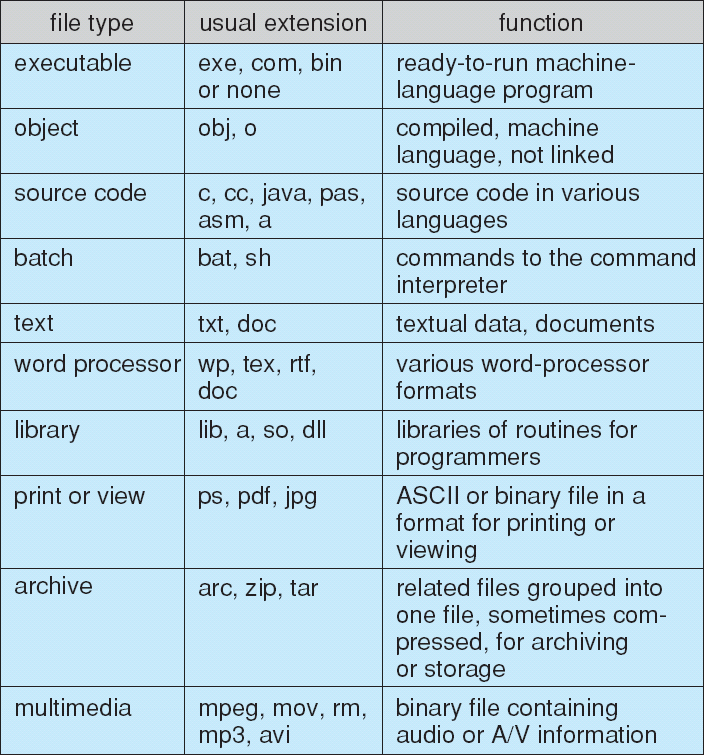
\includegraphics[scale=0.7]{img/C08_disco/tipos.png}
\caption{Diferentes tipos de archivos}
\label{fig:archivos_tipos}
\end{figure}

\subsection{Atributos}

Adicionalmente al contenido del archivo, este podrá tener diferentes
\textbf{atributos}, tales como:

\begin{itemize}
	\item \textbf{Nombre}: información en formato ``humano''.
	\item \textbf{Identificador}: etiquete (número) que lo identifica en el
sistema de archivos.
	\item \textbf{Tipo}: necesario para sistemas que soportan diferentes
tipos de archivos.
	\item \textbf{Ubicación}: puntero a la ubicación del archivo en el
dispositivo.
	\item \textbf{Tamaño}: tamaño actual del archivo.
	\item \textbf{Protección}: controla quien puede leer, escribir o
ejecutar el archivo.
	\item \textbf{Hora, fecha e identificación del usuario}: datos para
protección, seguridad y monitoreo de su uso.
\end{itemize}

A continuación se adjunta una lista con diferentes atributos de archivos
mediante la salida del comando \texttt{ls}.

% TODO quitar toda referencia a IET110 o UNAB del documento!!
\begin{verbatim}
delaf@goku:~/unab/iet110$ ls -lh
total 208K
drwxr-xr-x 3 delaf delaf 4,0K jun  4 04:00 apunte
drwxr-xr-x 3 delaf delaf 4,0K abr  9 21:01 diapos
-rw-r--r-- 1 delaf delaf  15K jun  2 15:51 iet110.ods
-rw-r--r-- 1 delaf delaf 166K nov 22  2011 IET110 Sistemas Operativos.pdf
drwxr-xr-x 5 delaf delaf 4,0K may 15 18:41 pruebas
drwxr-xr-x 5 delaf delaf 4,0K mar 25 02:38 so_juguete
drwxr-xr-x 2 delaf delaf 4,0K dic  1  2011 trabajos
-rw-r--r-- 1 delaf delaf  998 nov 22  2011 trabajo_v
\end{verbatim}

\subsection{Operaciones}

Sobre un archivo se pueden definir diversas operaciones, tales como: crear,
abrir, escribir, leer, reposicionar, eliminar, truncar o cerrar.
\texttt{Open(File)} busca en la estructura de directorios la entrada
\texttt{File} y mueve el contenido de la entrada a la memoria. De forma
contraría \texttt{Close} moverá de memoria a disco. ¿Qué sucedería si tuviese un
archivo de 100MB y solo 64MB de memoria principal?

\subsubsection{Abrir}
Para manejar un archivo abierto se requieren varias piezas de datos, estas en
conjunto permitirán traer el contenido deseado del archivo a la memoria
principal. Estas son:

\begin{itemize}
	\item \textbf{Puntero de archivo}: apunta a la última ubicación donde se
leyó o escribió el archivo, por cada uno de los procesos que tiene el archivo
abierto.
	\item \textbf{Contador de apertura}: cuenta el número de veces que el
archivo es abierto, permite remover los datos de la tabla de archivos una vez el
último proceso cierra el archivo.
	\item \textbf{Ubicación en el disco del archivo}: información para
acceder de forma física al archivo.
	\item \textbf{Permisos de acceso}: información respecto al modo de
acceso por proceso al archivo.
\end{itemize}

Algunos sistemas bloquean el acceso a los archivos si ya han sido abiertos por
otro proceso, esta es una forma de mediar con el acceso concurrente a un mismo
archivo. Cuando un archivo es abierto por primera vez el archivo es bloqueado,
luego cuando se quiere realizar una segunda apertura dos situaciones pueden
ocurrir: se puede denegar directamente el acceso al archivo o bien se puede
avisar que el archivo esta abierto y que el usuario elija que hacer, por ejemplo
abrirlo como solo lectura.

\subsection{Métodos de acceso}
Los métodos de acceso definen como se trabajara con el archivo, ya sea para
operaciones de lectura o de escritura.

\subsubsection{Acceso secuencial}
En este tipo de acceso el archivo es abierto y leído de forma continua hasta que
el archivo termina. Si se quiere leer algo nuevamente se debe volver al inicio y
empezar nuevamente.

\begin{verbatim}
/* operaciones */
read next
write next
reset
\end{verbatim}

En la figura \ref{fig:acceso_secuencial} se puede apreciar como el acceso
secuencial opera sobre un archivo. Donde desde una posición actual solo se pude
leer/escribir lo siguiente o volver al inicio.

\begin{figure}[htbp]
\centering
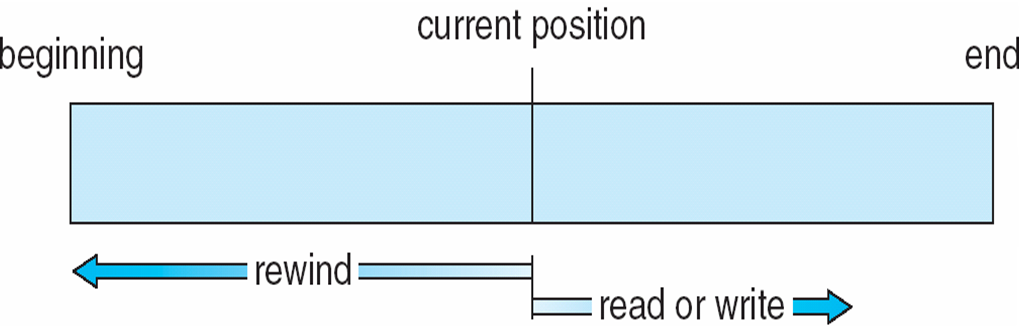
\includegraphics[scale=0.5]{img/C08_disco/acceso_secuencial.png}
\caption{Acceso secuencial a un archivo}
\label{fig:acceso_secuencial}
\end{figure}

\subsubsection{Acceso directo}
En el acceso directo se puede controlar directamente la posición del cursor
dentro del archivo, de esta forma se puede ir a una posición específica sin
tener que recorrer (leer) todo el archivo desde el inicio.

\begin{verbatim}
/* operaciones */
read n
write n
position to n
\end{verbatim}

Utilizando el acceso directo se puede simular el acceso secuencial como se ve en
la figura \ref{fig:acceso_secuencial_simulado}.

\begin{figure}[htbp]
\centering
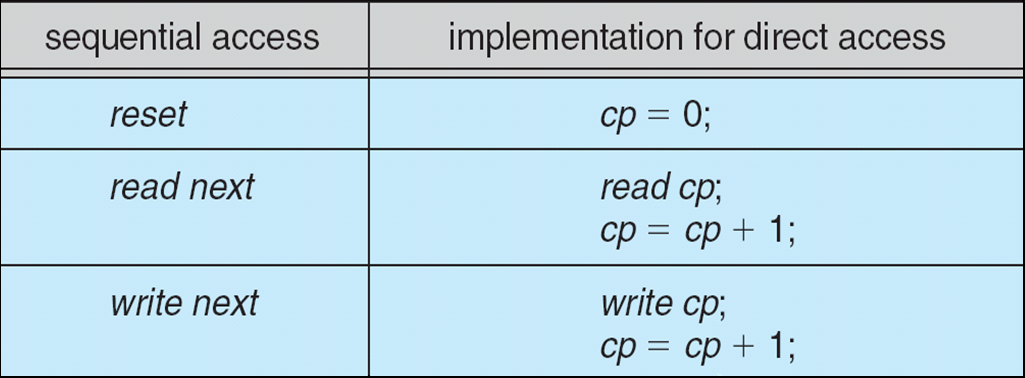
\includegraphics[scale=0.5]{img/C08_disco/acceso_secuencial_simulado.png}
\caption{Acceso secuencial simulado con acceso directo}
\label{fig:acceso_secuencial_simulado}
\end{figure}

\section{Estructura del disco}
Un disco puede ser dividido en particiones. Eventualmente estos discos o
particiones pueden ser protegidos ante fallas utilizando algún sistema, como
RAID.

Las particiones, que son las que se formatean, también son conocidas como
minidisks o slices (FreeBSD). En general la información de los discos es
guardada en una tabla de particiones, la cual permite a lo más guardar la
información de 4 particiones. Por esta razón un disco duro puede contener como
máximo 4 particiones primarias o bien 3 primarias y 1 extendida, donde la
extendida puede contener más particiones, pero lógicas.

Para utilizar el disco existen dos alternativas, escribir directamente en el
disco secuencias de bytes, en este caso se habla de un disco tipo RAW (sin un
sistema de archivo) o bien formateado con un sistema de archivos (como ext4,
reiserfs, jfs, xfs, fat, ntfs). La entidad que contiene al sistema de archivos
es conocida como un volumen, donde cada uno lleva un historial de la información
del sistema de archivos en una tabla de contenido del volumen. Así como hay
sistemas de archivos de propósito general hay aquellos que son sistemas de
archivo de propósito especial o específico, frecuentemente relacionados a un
sistema operativo

\section{Estructura de directorios}
Una estructura de directorios no es más que una colección de nodos conteniendo
información acerca de todos los archivos que contienen. Tanto la estructura de
directorio como los archivos residen en el disco, y ambas son necesarias para el
correcto funcionamiento del sistema de archivos. Por lo anterior, un respaldo
debe incluir las dos: archivos y estructura de directorios.

\subsection{Operaciones}
Sobre un directorio se pueden definir diversas operaciones, tales como: buscar
un archivo, crear un archivo, borrar un archivo, listar el contenido de un
directorio, renombrar un archivo o navegar por el sistema de archivos.

\subsection{Organización de los directorios}
El objetivo de dar una organización, orden o jerarquía a los directorios tiene
relación con:

\begin{itemize}
	\item \textbf{Eficiencia}: poder ubicar un archivo rápidamente.
	\item \textbf{Nombres}: dos o más usuarios podrían tener el mismo nombre
para diferentes archivos o bien el mismo archivo tener diferentes nombres.
	\item \textbf{Agrupar}: agrupar los archivos por propiedades, usos o
tipos (ej: binarios, configuraciones, datos variables, etc).
\end{itemize}

\subsubsection{Nivel simple}
En este caso solo existe un nivel de directorios, ver figura
\ref{fig:jerarquia_nivel_simple}. Aquí los mayores problemas son los nombres de
los archivos y la baja capacidad de agrupamiento.

\begin{figure}[htbp]
\centering
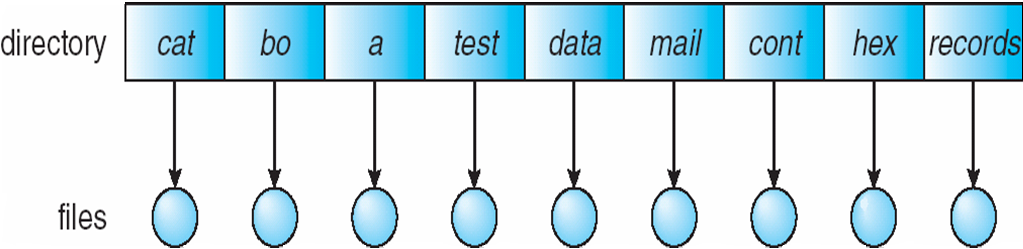
\includegraphics[scale=0.5]{img/C08_disco/jerarquia_nivel_simple.png}
\caption{Jerarquía de directorios simple}
\label{fig:jerarquia_nivel_simple}
\end{figure}

\subsubsection{Dos niveles}
En este caso se definen directorios separados para cada usuario, ver figura
\ref{fig:jerarquia_dos_niveles}. Esto permite tener el mismo nombre de archivo
para diferentes usuarios y provee de una búsqueda eficiente. Sin embargo las
capacidades de agrupar son muy limitadas.

\begin{figure}[htbp]
\centering
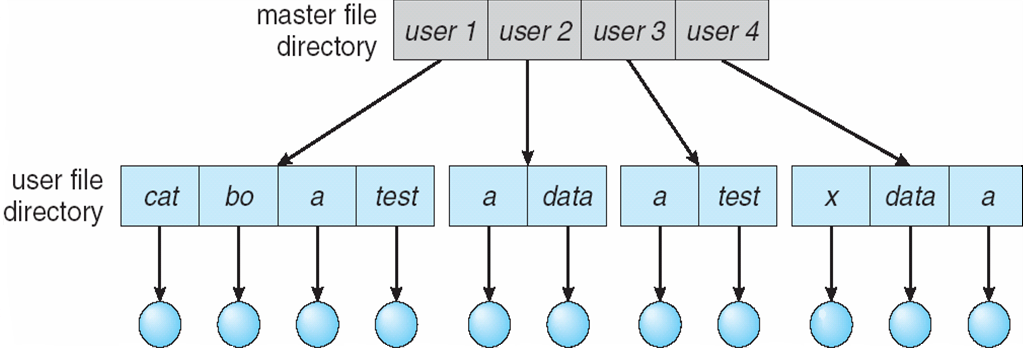
\includegraphics[scale=0.5]{img/C08_disco/jerarquia_dos_niveles.png}
\caption{Jerarquía de directorios con dos niveles}
\label{fig:jerarquia_dos_niveles}
\end{figure}

\subsubsection{Jerarquía en árbol}
En este tipo se crean ``infinitos'' niveles de subdirectorios, tantos como sean
necesarios, ver figura \ref{fig:jerarquia_arbol}. Provee de una búsqueda
eficiente, permite tener nombres de archivos repetidos y permite entregar
capacidades de agrupamiento.

\begin{figure}[htbp]
\centering
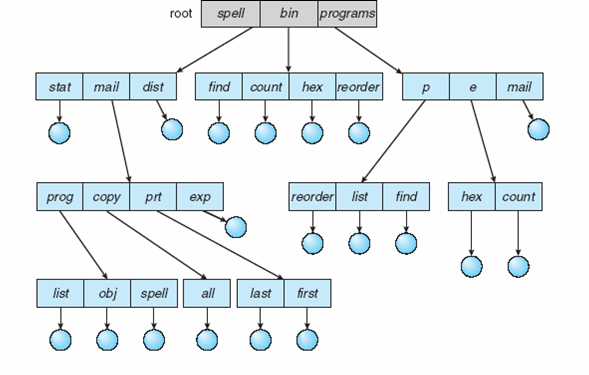
\includegraphics[scale=0.8]{img/C08_disco/jerarquia_arbol.png}
\caption{Jerarquía de directorios en árbol}
\label{fig:jerarquia_arbol}
\end{figure}

En este tipo de estructura de definen dos formas de navegar por el árbol de
directorios, mediante \textbf{rutas absolutas} que parten desde la raíz del
árbol o mediante \textbf{rutas relativas} que parten desde donde uno se
encuentra ``parado'' en el árbol.

Respecto al borrado de archivos o directorios, esta debe ser realizada de forma
recursiva, ya que se deben ir quitando las referencias entre directorios y
archivos de tal forma de no dejar nodos o hojas sin un nodo padre.

\section{Montaje}
Un sistema de archivos debe ser montado antes de poder ser accedido. Este
proceso se lleva acabo ``tomando'' el volumen no montado y ``ubicándolo'' en un
punto de montaje. Este punto de montaje corresponderá a algún directorio dentro
del sistema de archivos.

Si se llega a montar un volumen sobre un directorio que ya contiene archivos u
otros directorios estos no se perderán, solo quedarán inaccesibles hasta que el
volumen sea desmontado.

\section{Compartición}
Para compartir un archivo (o directorio) dentro del árbol de directorio se
pueden utilizar \textit{aliases} para nombrar a un mismo elemento en diferentes
partes del árbol.

En la figura \ref{fig:archivos_enlaces} se puede apreciar la compartición donde
un mismo archivo se encuentra en dos carpetas \texttt{count} y de forma similar
dos carpetas \texttt{w} y \texttt{words} apuntan a una misma llamada
\texttt{list}.

\begin{figure}[htbp]
\centering
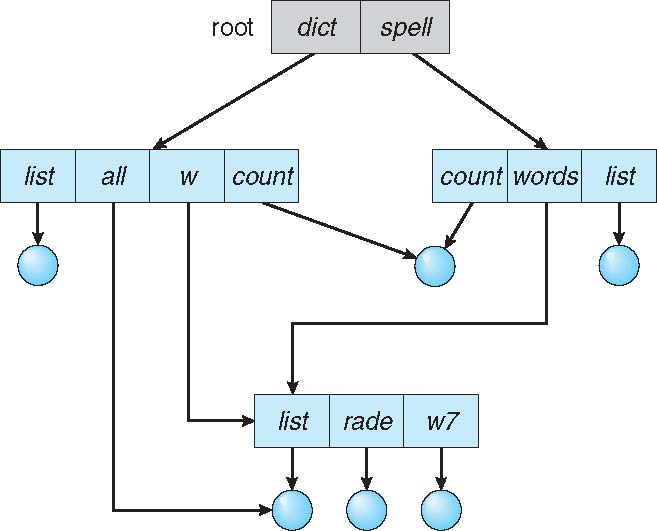
\includegraphics[scale=1]{img/C08_disco/enlaces.jpg}
\caption{Enlaces}
\label{fig:archivos_enlaces}
\end{figure}

Lo anterior es conocido como un enlace, lo cual será otro nombre (un puntero) a un archivo ya existente. Cuando se quiera acceder al enlace se deberá resolver siguiendo el puntero para localizar el archivo. Se definen dos tipos de enlaces:

\begin{enumerate}[i.]
	\item Enlaces simbólicos:
	\begin{itemize}
		\item Tamaño del enlace, tamaño de la ruta hacia el archivo.
		\item Apunta a una ruta en el sistema de archivos.
		\item Puede ser utilizado entre diferentes sistemas de archivos.
	\end{itemize}
	\item Enlaces duros
	\begin{itemize}
		\item Apunta al dispositivo de almacenamiento.
		\item Tamaño del enlace, tamaño del archivo.
		\item Solo puede ser utilizado en un mismo sistema de archivo.
	\end{itemize}
\end{enumerate}

\subsection{Protección}

Compartir archivos en un sistema multiusuarios es una tarea deseable, pero se debe considerar un esquema de protección para evitar que cualquier usuario pueda realizar cualquier tipo de operación sobre los archivos.

El propietario del archivo debe ser capaz de controlar ¿qué puede ser hecho? y ¿por quién puede ser hecho?. Para esto se utiliza el identificador del usuario (UID) y de grupo (GID) permitiendo definir los permisos que disponen cada uno de los usuarios del sistema sobre los archivos y directorios. Se definen tres tipos básicos de permisos: lectura (read), escritura (write) y ejecución (execute)

A continuación se explica la salida del comando \texttt{ls -l} que involucra los permisos recién descritos:

\begin{verbatim}
-rw-r--r--  1 usuario grupo    289 nov 20 23:08 archivo
- -  -  -   -                   -   -
| |  |  |   |                   |   |
| |  |  |   |                   |   +----- fecha de modificación
| |  |  |   |                   +--------- tamaño
| |  |  |   +----------------------------- enlaces duros
| |  |  +--------------------------------- permisos otros
| |  +------------------------------------ permisos grupo
| +--------------------------------------- permisos usuario
+----------------------------------------- tipo (común '–' o 'd')
\end{verbatim}


\section{Ejercicios y preguntas}
\begin{enumerate}
	\item Nombre 5 atributos de un archivo.
	\item Explique las partes involucradas en la apertura de un archivo.
	\item ¿Cuál es la diferencia entre el método de acceso secuencial y directo hacia un archivo?.
	\item ¿Se puede simular el acceso secuencial a un archivo con acceso directo?, explique.
	\item ¿Se puede simular el acceso directo a un archivo con acceso secuencial?, explique.
	\item ¿Cuántas particiones primarias se pueden crear en un disco? ¿por qué?.
	\item ¿Qué implica usar un disco como RAW?.
	\item ¿Cuales son los objetivos de la organización del disco?.
	\item ¿Por qué la estructura jerárquica simple no cumple con los objetivos?.
	\item ¿Cuál es la diferencia entre rutas relativas y rutas absolutas?.
	\item ¿Qué es el proceso de montaje?.
	\item ¿Cuál es la diferencia entre enlaces simbólicos y duros?.
	\item ¿Cuáles son los tres permisos definidos para un archivo o directorio?.
\end{enumerate}

\section{Referencias}
\begin{itemize}
	\item Sistemas Operativos, Segunda Edición, Andrew Tanenbaum, Capítulo 5.
	\item Sistemas Operativos, Quinta Edición, Abraham Silberschatz y Peter Baer Galvin, Capítulo 10 y 11.
	\item Sistemas Operativos, Segunda Edición, William Stallings, Capítulo 10 y 11.
\end{itemize}


% CAPÍTULO 9 PROTECCIÓN: 
%
% Apunte de Sistemas Operativos
% Copyright (C) 2014 Esteban De La Fuente Rubio (esteban[at]delaf.cl)
%
% Permission is granted to copy, distribute and/or modify this document
% under the terms of the GNU Free Documentation License, Version 1.3
% or any later version published by the Free Software Foundation;
% with no Invariant Sections, no Front-Cover Texts, and no Back-Cover Texts.
% A copy of the license is included in the section entitled "GNU
% Free Documentation License".
%
% Link: http://www.gnu.org/copyleft/fdl.html
%

% PROTECCIÓN Y SEGURIDAD
\chapter{Protección y seguridad}
\label{proteccion}
Controlar el acceso a los recursos es una de las tareas más importantes del
sistema operativo, sin embargo no solo debe asegurar que estos accesos sean
sincronizados y sin problemas de concurrencia (como ya se discutió
anteriormente), sino que también debe asegurar que solo accedan a los recursos
quienes estén autorizados a hacerlo.

En un modelo de protección el computador simplemente es un conjunto de objetos,
ya sean estos físicos (hardware) o lógicos (software o datos). Donde cada objeto
puede ser identificado por un nombre único y tendrá asociado un conjunto
definido de operaciones.

Entonces, el problema de la protección consiste en asegurar que cada objeto sea
accedido correctamente, mediante las operaciones definidas, y solo por aquellos
procesos que tienen permitido hacerlo.

En este capítulo se hablará de conceptos de protección genéricos, los cuales
pueden aplicarse a un sistema operativo o bien a cualquier otro tipo de sistema,
ya sea o no computacional.

\section{Principios de protección}
En protección se considera generalmente el \textbf{principio del menor
privilegio}, esto implica que un programa, usuario o sistema en general deberá
tener los privilegios mínimos para poder realizar las tareas que deba hacer.

Supongamos una secretaria en un banco, sería un error dar a ella acceso a la
bóveda si de lo único que se tiene que encargar es atender las consultas de los
clientes. Para realizar su tarea, ``atender clientes'', la secretaria solo
necesita acceso a una determinada área del banco, no a todo este.

Esto tiene mucha relación con la idea de \textbf{denegar todo y permitir
algunos}, donde se evita que el usuario pueda hacer cualquier cosa en el sistema
y solo se le conceden accesos específicos según lo que debe realizar.

Este tipo de política limita el daño si la ejecución del proceso tiene algún
error, ya que de haberlo a lo más podrá afectar a aquellos objetos con los que
tenía permitido interactuar.

La forma de utilizar esta política es concediendo los privilegios de forma
\textbf{estática}, o sea el proceso durante toda su ejecución tendrá los mismos
privilegios. O bien de forma \textbf{dinámica} donde el proceso podrá cambiar
sus privilegios según vaya requiriendo, este concepto es conocido como
\textbf{escalada de privilegios}.

Se deberá determinar a que nivel de detalle se manejarán los privilegios, un
nivel más tosco implicará un manejo más simple, sin embargo se deberá realizar a
grandes rasgos o abarcando muchas operaciones u objetos. Un manejo más fino será
más complejo de administrar, pero permitirá definir con precisión los
privilegios para los procesos.

\section{Dominios}
Un dominio definirá un conjunto de derechos de acceso que el proceso (o usuario)
tienen sobre determinados objetos, especificando para cada uno de estos objetos
las posibles operaciones que el proceso puede realizar sobre el mismo.

En la figura \ref{fig:proteccion_dominios} se puede observar un ejemplo con tres
dominios, cada uno con un conjunto de derechos de acceso y las operaciones que
pueden realizar sobre cada uno de los objetos. Notar que los dominios $D_2$ y
$D_3$ comparten una misma operación sobre un objeto.

\begin{figure}[htbp]
\centering
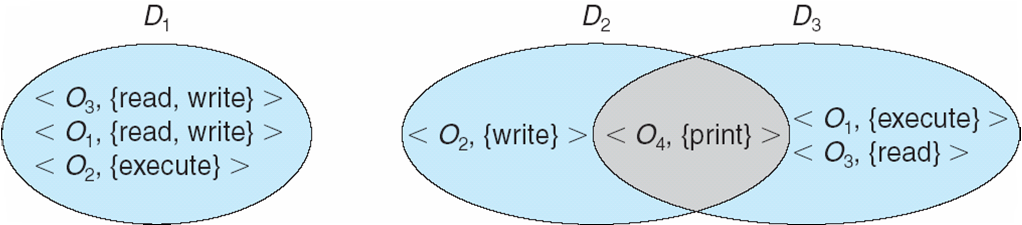
\includegraphics[scale=0.6]{img/C09_proteccion/dominios.png}
\caption{Ejemplo de dominios y sus conjuntos de derechos de acceso}
\label{fig:proteccion_dominios}
\end{figure}

\subsection{Dominios en sistemas \textit{like Unix}}
En sistemas operativos \textit{like Unix}, los dominios están definidos por el
identificador del usuario (UID) y el o los grupos a los que pertenece el usuario
(GID).

El cambio de dominio, específicamente el cambio de dominio definido por el UID,
puede ser realizado de diferentes maneras:
\begin{enumerate}[i.]

\item \textbf{Vía sistema de archivos}: cada archivo tiene asociado un bit
(\textit{setuid bit}) que permite indicar que cuando el archivo sea ejecutado se
realice con el dominio del dueño del archivo y no con el dominio de quien
ejecuta el archivo.

\item \textbf{Vía contraseñas}: comando \texttt{su} que permite cambiar a otro
dominio de usuario.

\item \textbf{Vía comandos}: comando \texttt{sudo} que ejecuta un comando
específico utilizando otro domino. Generalmente el otro dominio es el del
usuario con UID 0 (root), pero no necesariamente tiene que ser ese dominio.

\end{enumerate}

\section{Matriz de acceso}
Las políticas de protección se pueden ver como una matriz (tabla) donde las
filas representan los dominios, las columnas representan los objetos y cada
$casilla_{ij}$ de la tabla corresponde a las operaciones que un proceso
ejecutándose en el dominio $i$ puede realizar sobre el objeto $j$.

En la figura \ref{fig:matriz_acceso} se puede observar un ejemplo de una matriz
de acceso donde, por ejemplo, el dominio $D_3$ puede leer el fichero $F_2$ pero
no el $F_1$. De la misma forma el único que puede imprimir es el dominio $D_2$.

\begin{figure}[htbp]
\centering
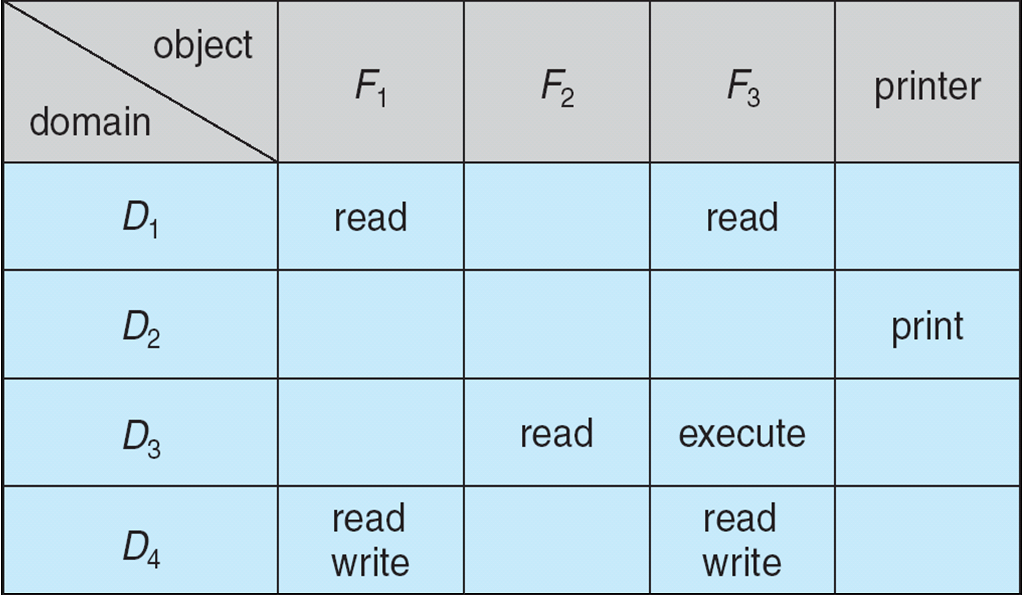
\includegraphics[scale=0.5]{img/C09_proteccion/matriz_acceso.png}
\caption{Ejemplo de matriz de acceso}
\label{fig:matriz_acceso}
\end{figure}

En general la forma de revisar la matriz de acceso es: si un proceso del dominio
$D_i$ trata de hacer una operación $X$ en el objeto $O_j$, entonces la operación
$X$ debe estar en la $casilla_{ij}$ en la matriz de acceso.

Se deben definir operaciones para agregar o quitar derechos de uso, algunas son:
\begin{itemize}
\item Definir propietario de $Objeto_j$.
\item Copiar operación desde $Objeto_j$ a $Objeto_k$.
\item Control: $Dominio_i$ puede modificar los accesos de $Dominio_h$.
\item Transferencia: del dominio $Dominio_i$ al $Dominio_h$.
\end{itemize}

Para definir las operaciones sobre dominios es necesario que el dominio sea
tratado como un objeto más dentro de la matriz de acceso, de esta forma se
tendrá algo similar al ejemplo de la figura \ref{fig:matriz_acceso_dominios}.

\begin{figure}[htbp]
\centering
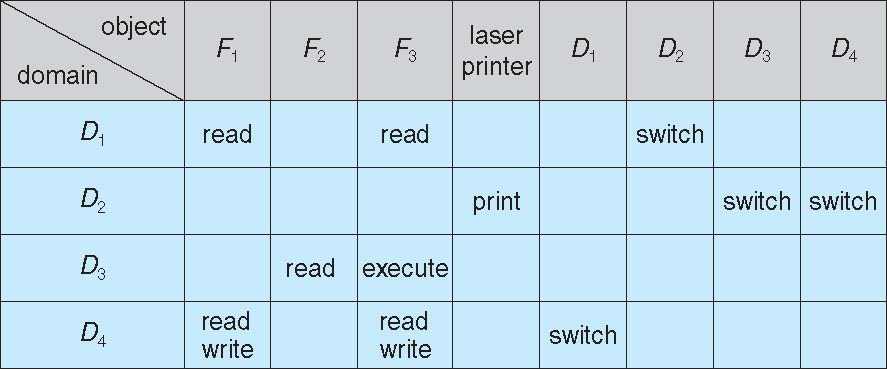
\includegraphics[scale=1.2]{img/C09_proteccion/matriz_acceso_dominios.jpg}
\caption{Ejemplo de matriz de acceso usando dominios como objetos}
\label{fig:matriz_acceso_dominios}
\end{figure}

Finalmente es importante mencionar que la matriz de acceso separa políticas de
mecanismos, teniendo que:
\begin{itemize}
\item Mecanismos:
\begin{itemize}
	\item Sistema operativo provee de matriz de acceso más reglas.
	\item Asegura que la matriz sea solo manipulada por agentes autorizados.
	\item Reglas de la matriz aplicadas estrictamente.
\end{itemize}
\item Políticas:
\begin{itemize}
	\item Usuario indica las políticas.
	\item Se define \textbf{¿quién puede acceder?} a que objeto y
	\textbf{¿en qué	modo?}.
\end{itemize}
\end{itemize}

\section{Ejercicios y preguntas}
\begin{enumerate}
\item Explique el principio del menor privilegio.
\item ¿Por qué es recomendable denegar todo y solo asignar los permisos
específicos que son requeridos?
\item Explique los métodos de asignación de privilegios estáticos y dinámicos.
\item ¿En qué consisten los dominios?.
\item ¿Qué son los derechos de acceso?.
\item ¿Cuáles son las tres vías para hacer un cambio de dominio en Unix?.
\item ¿Qué es la matriz de acceso?.
\item ¿Qué representan las filas y columnas en la matriz de acceso?.
\item ¿Por qué se podría querer tratar a los dominios como objetos en la matriz
de acceso?.
\end{enumerate}

\section{Referencias}
\begin{itemize}
\item Sistemas Operativos, Quinta Edición, Abraham Silberschatz y Peter Baer
Galvin, Capítulo 19 y 20.
\item Sistemas Operativos, Segunda Edición, William Stallings, Capítulo 14.
\end{itemize}


% ANEXOS
\renewcommand{\appendixname}{Anexo}
\appendix

% ANEXO A: MÁQUINAS VIRTUALES
\include{anexos/A01_maquinas_virtuales}

\end{document}
